\pdfoutput=1
\documentclass[11pt,a4paper]{article}
\usepackage[T1]{fontenc}
\usepackage[utf8]{inputenc}
\usepackage{amsmath,amssymb,amsthm}
\usepackage{mathtools}
\usepackage{mathdots}
\usepackage{jheppub}
\usepackage{enumitem}
\usepackage{tikz}
\usetikzlibrary{arrows.meta,calc,decorations.markings,decorations.pathreplacing,patterns,positioning}
\hypersetup{hypertexnames=false,colorlinks=true,linkcolor=black,citecolor=black,urlcolor=blue}

% Edited JHEP edition of I. Grojnowski, "Introduction to Lie algebras and
% their representations", Part III lectures, Cambridge, Michaelmas 2010,
% typeset by E. Yudovina. Source PDF: originals/grojnowski-lie-algebras.pdf.
% Every change of mathematical substance is listed in ../CORRECTIONS.md.
%
% Numbering follows the original: theorem-like statements share one counter
% per section, examples have their own counter per section, and exercises
% are numbered consecutively through the whole text.

% ---------------------------------------------------------------- theorems
\theoremstyle{plain}
\newtheorem{theorem}{Theorem}[section]
\newtheorem{lemma}[theorem]{Lemma}
\newtheorem{proposition}[theorem]{Proposition}
\newtheorem{corollary}[theorem]{Corollary}
\newtheorem*{claim}{Claim}
\theoremstyle{definition}
\newtheorem{properties}[theorem]{Properties}
\newtheorem{example}{Example}[section]
\newtheorem{exercise}{Exercise}
\newtheorem*{definition}{Definition}
\theoremstyle{remark}
\newtheorem*{remark}{Remark}
\newenvironment{sketch}[1]{\begin{proof}[Sketch #1]}{\end{proof}}

\setlist[enumerate]{label=(\arabic*),leftmargin=*,topsep=2pt,itemsep=1pt}
\setlist[itemize]{topsep=2pt,itemsep=1pt}
\newlist{alist}{enumerate}{1}
\setlist[alist]{label=(\alph*),leftmargin=*,topsep=2pt,itemsep=1pt}

\setlength{\emergencystretch}{2.5em}

\newcommand{\lecture}[1]{\par\medskip\noindent\textbf{Lecture #1.}\enspace\ignorespaces}

% ------------------------------------------------------------------ fields
\newcommand{\C}{\mathbb{C}}
\newcommand{\R}{\mathbb{R}}
\newcommand{\Z}{\mathbb{Z}}
\newcommand{\Q}{\mathbb{Q}}
\newcommand{\N}{\mathbb{N}}
\newcommand{\Fpbar}{\overline{\mathbb{F}}_p}
\newcommand{\PP}{\mathbb{P}}

% ------------------------------------------------------------- Lie algebras
\newcommand{\g}{\mathfrak{g}}
\newcommand{\h}{\mathfrak{h}}
\newcommand{\at}{\mathfrak{t}}
\newcommand{\fa}{\mathfrak{a}}
\newcommand{\fb}{\mathfrak{b}}
\newcommand{\fn}{\mathfrak{n}}
\newcommand{\fr}{\mathfrak{r}}
\newcommand{\fm}{\mathfrak{m}}
\newcommand{\fs}{\mathfrak{s}}
\newcommand{\fz}{\mathfrak{z}}
\newcommand{\Heis}{\mathfrak{H}}
\newcommand{\gl}{\mathfrak{gl}}
\renewcommand{\sl}{\mathfrak{sl}}
\newcommand{\so}{\mathfrak{so}}
\newcommand{\spl}{\mathfrak{sp}}
\newcommand{\gbar}{\overline{\mathfrak{g}}}
\newcommand{\gtil}{\widetilde{\mathfrak{g}}}
\newcommand{\U}{\mathcal{U}}

% --------------------------------------------------------------- operators
\DeclareMathOperator{\ad}{ad}
\DeclareMathOperator{\tr}{trace}
\DeclareMathOperator{\End}{End}
\DeclareMathOperator{\Hom}{Hom}
\DeclareMathOperator{\Aut}{Aut}
\DeclareMathOperator{\Mat}{Mat}
\DeclareMathOperator{\Lie}{Lie}
\DeclareMathOperator{\Rep}{Rep}
\DeclareMathOperator{\Span}{Span}
\DeclareMathOperator{\Spec}{Spec}
\DeclareMathOperator{\Sym}{Sym}
\DeclareMathOperator{\ch}{ch}
\DeclareMathOperator{\wt}{wt}
\DeclareMathOperator{\gr}{gr}
\DeclareMathOperator{\CT}{CT}
\DeclareMathOperator{\htt}{ht}
\DeclareMathOperator{\Id}{Id}
\DeclareMathOperator{\Spin}{Spin}
\DeclareMathOperator{\rank}{rank}
\DeclareMathOperator{\charac}{char}
\newcommand{\dimq}{\dim_q}
\newcommand{\te}{\tilde{e}}
\newcommand{\tf}{\tilde{f}}
\newcommand{\eps}{\epsilon}
\newcommand{\ip}[2]{\langle #1,#2\rangle}
\newcommand{\cv}{^{\vee}}
\newcommand{\bx}[1]{\mbox{\fboxsep=2pt\fbox{$#1$}}}
\newcommand{\xto}[1]{\xrightarrow[#1]{}}
\newcommand{\setc}[2]{\{#1 \mid #2\}}

% ---------------------------------------------------------- figure helpers
\tikzset{
  dot/.style={circle,fill,inner sep=1.6pt},
  node/.style={circle,draw,inner sep=0pt,minimum size=9pt,fill=white},
  aff/.style={circle,draw,inner sep=0pt,minimum size=9pt,pattern=north east lines},
  root/.style={-{Stealth[length=6pt]},thick},
  cr1/.style={-{Stealth[length=5pt]},black},
  cr2/.style={-{Stealth[length=5pt]},red!80!black},
}
% a double or triple bond between nodes at #1 and #2 with an arrowhead
% pointing at the short root, here always the second argument
\newcommand{\dbond}[2]{%
  \draw[double distance=2.2pt] (#1) -- (#2);
  \draw[thick] ($(#1)!0.42!(#2)+(0,4pt)$) -- ($(#1)!0.58!(#2)$) -- ($(#1)!0.42!(#2)-(0,4pt)$);}
\newcommand{\tbond}[2]{%
  \draw ($(#1)+(0,2.4pt)$) -- ($(#2)+(0,2.4pt)$);
  \draw (#1) -- (#2);
  \draw ($(#1)-(0,2.4pt)$) -- ($(#2)-(0,2.4pt)$);
  \draw[thick] ($(#1)!0.42!(#2)+(0,5pt)$) -- ($(#1)!0.58!(#2)$) -- ($(#1)!0.42!(#2)-(0,5pt)$);}
% the sl_2 tensor product crystal L(n) (x) L(m) with n = 4, m = 6
\newcommand{\slcrystal}{%
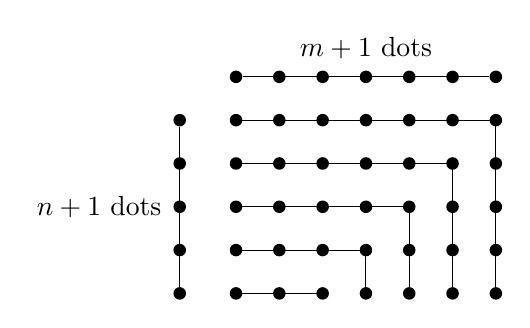
\begin{tikzpicture}[scale=0.55]
  \foreach \c in {0,...,6} \node[dot] (t\c) at (\c,1) {};
  \draw (t0) -- (t6);
  \node[above] at (3,1.2) {$m+1$ dots};
  \foreach \r in {0,...,4} \node[dot] (l\r) at (-1.3,-\r) {};
  \draw (l0) -- (l4);
  \node[left] at (-1.5,-2) {$n+1$ dots};
  \foreach \r in {0,...,4} {
    \pgfmathtruncatemacro{\last}{6-\r}
    \foreach \c in {0,...,6} \node[dot] at (\c,-\r) {};
    \draw (0,-\r) -- (\last,-\r) -- (\last,-4);
  }
\end{tikzpicture}}

\title{Introduction to Lie Algebras and their Representations}
\subheader{Part III lecture notes, University of Cambridge, Michaelmas 2010}
\author[a]{Ian Grojnowski}
\author[b]{with notes typeset by Elena Yudovina}
\affiliation[a]{DPMMS, University of Cambridge}
\affiliation[b]{Statistical Laboratory, University of Cambridge}
\emailAdd{I.Grojnowski@dpmms.cam.ac.uk}
\emailAdd{E.Yudovina@statslab.cam.ac.uk}
\abstract{These are notes from a Part III course given in Cambridge in the
autumn of 2010. They start from $\sl_2$ and its representations. From there
they go through the structure and classification of semisimple Lie algebras
over $\C$, root systems and Dynkin diagrams, highest-weight theory, Verma
modules and the Weyl character formula. The last lectures cover the principal
$\sl_2$, Kashiwara crystals and Littelmann paths. This edition corrects
misprints and mathematical slips in the 2011 typescript; the file
\texttt{CORRECTIONS.md} beside the source lists every change of substance.}

\begin{document}
\maketitle
\flushbottom

\section{Introduction, motivation, etc.}

\lecture{1} For most of this lecture, we will be motivating why we care about
Lie algebras and why they are defined the way they are. If there are sections
of it that don't make sense, they can be skipped (although if none of it makes
sense, you should be worried).

Connected Lie groups are groups which are also differentiable manifolds. The
simple algebraic groups over algebraically closed fields (which form a nice
class of Lie groups) are:
\begin{align*}
  SL(n) &= \setc{A \in \Mat_n}{\det A = 1},\\
  SO(n) &= \setc{A \in SL_n}{AA^T = I},\\
  Sp(2n) &= \setc{A \in SL_{2n}}{A \text{ preserves a symplectic form}},
\end{align*}
and exactly $5$ others (as we will actually see!). (We are ignoring finite
centres, so $\Spin(n)$, the double cover of $SO(n)$, is missing.)

\begin{remark}
Each of these groups has a maximal compact subgroup. For example, $SU(n)$ is
the maximal compact subgroup of $SL_n(\C)$, while $SO_n(\R)$ is the maximal
compact subgroup of $SO_n(\C)$. These are themselves Lie groups, of course.
The representations of the maximal compact subgroup are the same as the
algebraic representations of the simple algebraic group, which in turn are the
same as the finite-dimensional representations of its (the simple algebraic
group's) Lie algebra. These last are what we study.
\end{remark}

Lie groups are complicated objects: for example, $SU_2(\C)$ is homeomorphic to
a $3$-sphere, and $SU_n$ is a twisted product of a $3$-sphere, a $5$-sphere,
\dots, a $(2n-1)$-sphere. Thus, studying Lie groups requires some amount of
algebraic topology and a lot of algebraic geometry. We want to replace these
``complicated'' disciplines by the ``easy'' discipline of linear algebra.

Therefore, instead of a Lie group $G$ we will be considering $\g = T_IG$, the
tangent space to $G$ at the identity.

\begin{definition}
A \emph{linear algebraic group} is a subgroup of some $GL_n$ defined by
polynomial equations in the matrix coefficients.
\end{definition}

We see that the examples above are linear algebraic groups.

\begin{remark}
It is not altogether obvious that this is an intrinsic characterisation (it
would be nice not to depend on the embedding into $GL_n$). The intrinsic
characterisation is as ``affine algebraic groups'', that is, groups which are
affine algebraic varieties and for which multiplication and inverse are
morphisms of affine algebraic varieties. One direction of this identification
is relatively easy (we just need to check that multiplication and inverse
really are morphisms); in the other direction, we need to show that any affine
algebraic group has a faithful finite-dimensional representation, i.e.\ embeds
in $GL(V)$. This involves looking at the ring of functions and doing something
with it.
\end{remark}

We will now explain a tangent space if you haven't met with it before.

\begin{example}
Let's pretend we're physicists, since we're in their building anyway. Let
$G = SL_2$, and let $|\eps| \ll 1$. Then for
\[
  g = \begin{pmatrix} 1 & \\ & 1 \end{pmatrix}
      + \eps \begin{pmatrix} a & b \\ c & d \end{pmatrix}
      + \text{higher-order terms}
\]
to lie in $SL_2$, we must have $\det g = 1$, or
\[
  1 = \det \begin{pmatrix} 1 + \eps a & \eps b \\ \eps c & 1 + \eps d \end{pmatrix}
      + \text{h.o.t.}
    = 1 + \eps(a + d) + \eps^2(\text{junk}) + \text{h.o.t.}
\]
Therefore, to have $g \in G$ we need to have $a + d = 0$.
\end{example}

To do this formally, we define the \emph{dual numbers}
\[
  E = \C[\eps]/\eps^2 = \setc{a + b\eps}{a, b \in \C}.
\]
For a linear algebraic group $G$, we consider
\[
  G(E) = \setc{A \in \Mat_n(E)}{A \text{ satisfies the polynomial equations defining } G \subset GL_n}.
\]
For example,
\[
  SL_2(E) = \Bigl\{ \begin{pmatrix} \alpha & \beta \\ \gamma & \delta \end{pmatrix}
     \Bigm| \alpha, \beta, \gamma, \delta \in E,\ \alpha\delta - \beta\gamma = 1 \Bigr\}.
\]
The natural map $E \to \C$, $\eps \mapsto 0$ gives a projection
$\pi\colon G(E) \to G$. We define the Lie algebra of $G$ as
\[
  \g \cong \pi^{-1}(I) \cong \setc{X \in \Mat_n(\C)}{I + \eps X \in G(E)}.
\]
In particular,
\[
  \sl_2 = \Bigl\{ \begin{pmatrix} a & b \\ c & d \end{pmatrix} \in \Mat_2(\C)
     \Bigm| a + d = 0 \Bigr\}.
\]

\begin{remark}
$I + \eps X$ represents an ``infinitesimal change at $I$ in the direction
$X$''. Equivalently, it is a map $\Spec \C[\eps]/\eps^2 \to G$, the
first-order germ of a curve through $I$.
\end{remark}

\begin{exercise}
(Do this only if you already know what a tangent space and tangent bundle
are.) Show that $G(E) = TG$ is the tangent bundle to $G$, and $\g = T_IG$ is
the tangent space to $G$ at $I$.
\end{exercise}

\begin{example}
Let $G = GL_n = \setc{A \in \Mat_n}{A^{-1} \text{ exists}}$.
Claim:
\begin{align*}
  G(E) &:= \setc{\tilde A \in \Mat_n(E)}{\tilde A^{-1} \text{ exists}}\\
       &= \setc{A + B\eps}{A, B \in \Mat_n(\C),\ A^{-1} \text{ exists}}.
\end{align*}
Indeed, $(A + B\eps)(A^{-1} - A^{-1}BA^{-1}\eps) = I$.
\end{example}

\begin{remark}
It is not obvious that $GL_n$ is itself a linear algebraic group (what are the
polynomial equations for ``determinant is non-zero''?). However, we can think
of $GL_n \subset \Mat_{n+1}$ as
\[
  \Bigl\{ \begin{pmatrix} A & \\ & \lambda \end{pmatrix}
     \Bigm| \det(A) \cdot \lambda = 1 \Bigr\}.
\]
\end{remark}

\begin{example}
$G = SL_n(\C)$.
\end{example}

\begin{exercise}
$\det(I + \eps X) = 1 + \eps \tr(X)$.
\end{exercise}

As a corollary to the exercise, $\sl_n = \setc{X \in \Mat_n}{\tr(X) = 0}$.

\begin{example}
$G = O_n(\C) = \setc{A}{AA^T = I}$. Then
\begin{align*}
  \g &:= \setc{X \in \Mat_n(\C)}{(I + \eps X)(I + \eps X)^T = I}\\
     &= \setc{X \in \Mat_n(\C)}{I + \eps(X + X^T) = I}\\
     &= \setc{X \in \Mat_n(\C)}{X + X^T = 0},
\end{align*}
the antisymmetric matrices. Now, if $X + X^T = 0$ then $2\tr(X) = 0$, and
since we're working over $\C$ and not in characteristic $2$, we conclude
$\tr(X) = 0$. Therefore, this is also the Lie algebra of $SO_n$.

This is not terribly surprising, because topologically $O_n$ has two connected
components corresponding to determinant $+1$ and $-1$ (they are images of each
other via a reflection). Since $\g = T_IG$, it cannot see the $\det = -1$
component, so this is expected.
\end{example}

The above example prompts the question: what exactly is it in the structure of
$\g$ that we get from $G$ being a group?

The first thing to note is that $\g$ does \emph{not} get a multiplication.
Indeed, $(I + A\eps)(I + B\eps) = I + (A + B)\eps$, which has nothing to do
with multiplication.

The operation that turns out to generalise nicely is the commutator,
$(P, Q) \mapsto PQP^{-1}Q^{-1}$. Taken as a map $G \times G \to G$ that sends
$(I, I) \mapsto I$, this should give a map $T_IG \times T_IG \to T_IG$ by
differentiation.

\begin{remark}
Generally, differentiation gives a \emph{linear} map, whereas what we will get
is a \emph{bilinear} map. This is because we will in fact differentiate each
coordinate: i.e.\ first differentiate the map $f_P\colon G \to G$,
$Q \mapsto PQP^{-1}Q^{-1}$ with respect to $Q$ to get a map
$\tilde f_P\colon \g \to \g$ (with $P \in G$ still) and then differentiate
again to get a map $\g \times \g \to \g$.
\end{remark}

What is this map? Let $P = I + A\eps$, $Q = I + B\delta$ where
$\eps^2 = \delta^2 = 0$ but $\eps\delta \neq 0$. Then
\begin{align*}
  PQP^{-1}Q^{-1} &= (I + A\eps)(I + B\delta)(I - A\eps)(I - B\delta)\\
                 &= I + (AB - BA)\eps\delta.
\end{align*}
Thus, the binary operation on $\g$ should be $[A, B] = AB - BA$.

\begin{definition}
The \emph{bracket} of $A$ and $B$ is $[A, B] = AB - BA$.
\end{definition}

\begin{exercise}
Show that $(PQP^{-1}Q^{-1})^{-1} = QPQ^{-1}P^{-1}$ implies $[A, B] = -[B, A]$,
i.e.\ the bracket is skew-symmetric.
\end{exercise}

\begin{exercise}
Show that the associativity of multiplication in $G$ implies the \emph{Jacobi
identity}
\[
  0 = [[X, Y], Z] + [[Y, Z], X] + [[Z, X], Y].
\]
\end{exercise}

\begin{remark}
The meaning of ``implies'' in the above exercises is as follows: we want to
think of the bracket as the derivative of the commutator, not as the explicit
formula $[A, B] = AB - BA$ (which makes the skew-symmetry obvious, and the
Jacobi identity only slightly less so). For example, we could have started
working in a different category.
\end{remark}

We will now define our object of study.

\begin{definition}
Let $K$ be a field, $\charac K \neq 2, 3$. A \emph{Lie algebra} $\g$ is a
vector space over $K$ equipped with a bilinear map (\emph{Lie bracket})
$[\,,\,]\colon \g \times \g \to \g$ with the following properties:
\begin{enumerate}
  \item $[X, Y] = -[Y, X]$ (skew-symmetry);
  \item $[[X, Y], Z] + [[Y, Z], X] + [[Z, X], Y] = 0$ (Jacobi identity).
\end{enumerate}
\end{definition}

\lecture{2} Examples of the Lie algebra definition from last time:

\begin{example}\leavevmode
\begin{enumerate}
  \item $\gl_n = \Mat_n$ with $[A, B] = AB - BA$.
  \item $\so_n = \setc{A}{A + A^T = 0}$.
  \item $\sl_n = \setc{A}{\tr(A) = 0}$ (note that while $AB$ need not have
    trace $0$ for $A, B \in \sl_n$, we do have $\tr(AB) = \tr(BA)$, so
    $[A, B] \in \sl_n$ even though $AB \notin \sl_n$ in general).
  \item $\spl_{2n} = \setc{A \in \gl_{2n}}{JA^TJ^{-1} + A = 0}$, where $J$ is
    the symplectic form
    \[
      J = \begin{pmatrix}
            &&&&& 1\\
            &&&& \iddots &\\
            &&& 1 &&\\
            && -1 &&&\\
            & \iddots &&&&\\
            -1 &&&&&
          \end{pmatrix}.
    \]
  \item $\fb = \Biggl\{ \begin{pmatrix}
            * & * & \cdots & *\\
              & * & \cdots & *\\
              &   & \ddots & \vdots\\
              &   &        & *
          \end{pmatrix} \in \gl_n \Biggr\}$,
    the upper triangular matrices (the name is $\fb$ for Borel, but we don't
    need to worry about that yet).
  \item $\fn = \Biggl\{ \begin{pmatrix}
            0 & * & \cdots & *\\
              & 0 & \cdots & *\\
              &   & \ddots & \vdots\\
              &   &        & 0
          \end{pmatrix} \in \gl_n \Biggr\}$,
    the strictly upper triangular matrices (the name is $\fn$ for nilpotent,
    but we don't need to worry about that yet).
  \item For any vector space $V$, let $[\,,\,]\colon V \times V \to V$ be the
    zero map. This is the ``abelian Lie algebra''.
\end{enumerate}
\end{example}

\begin{exercise}\leavevmode
\begin{enumerate}
  \item Check directly that $\gl_n$ is a Lie algebra.
  \item Check that the other examples above are Lie subalgebras of $\gl_n$,
    that is, vector subspaces closed under $[\,,\,]$.
\end{enumerate}
\end{exercise}

\begin{example}
$\begin{pmatrix} * & * \\ * & 0 \end{pmatrix}$ is \emph{not} a Lie subalgebra
of $\gl_2$.
\end{example}

\begin{exercise}
Find the algebraic groups whose Lie algebras are given above.
\end{exercise}

\begin{exercise}
Classify all Lie algebras of dimension $3$. (You might want to start with
dimension $2$. I'll do dimension $1$ for you on the board: skew-symmetry of
the bracket means that the bracket is zero, so there is only the abelian one.)
\end{exercise}

\begin{definition}
A \emph{representation} of a Lie algebra $\g$ on a vector space $V$ is a
homomorphism of Lie algebras $\phi\colon \g \to \gl_V$. We say that $\g$
\emph{acts on} $V$.
\end{definition}

Observe that, above, our Lie algebras were defined with a (faithful)
representation in tow.

There is always a representation coming from the Lie algebra acting on itself
(it is the derivative of the group acting on itself by conjugation):

\begin{definition}
For $x \in \g$ define $\ad(x)\colon \g \to \g$ as $y \mapsto [x, y]$.
\end{definition}

\begin{lemma}
$\ad\colon \g \to \End \g$ is a representation (called the \emph{adjoint
representation}).
\end{lemma}

\begin{proof}
We need to check whether $\ad([x, y]) = \ad(x)\ad(y) - \ad(y)\ad(x)$, i.e.\
whether the equality holds when we apply it to a third element $z$. But
\[
  \ad([x, y])(z) = [[x, y], z]
\]
and
\[
  \ad(x)\ad(y)(z) - \ad(y)\ad(x)(z) = [x, [y, z]] - [y, [x, z]]
    = -[[y, z], x] - [[z, x], y].
\]
These are equal by the Jacobi identity.
\end{proof}

\begin{definition}
The \emph{centre} of $\g$ is
$\setc{x \in \g}{[x, y] = 0 \ \forall y \in \g} = \ker(\ad\colon \g \to \End \g)$.
\end{definition}

Thus, if $\g$ has no centre, then $\ad$ is an embedding of $\g$ into
$\End \g$ (and conversely, of course).

Is it true that every finite-dimensional Lie algebra embeds into some $\gl_V$,
i.e.\ is linear? (Equivalently, is it true that every finite-dimensional Lie
algebra has a faithful finite-dimensional representation?) We see that if $\g$
has no centre, then the adjoint representation makes this true. On the other
hand, if we look inside $\gl_2$, then
$\fn = \bigl(\begin{smallmatrix} 0 & * \\ 0 & 0 \end{smallmatrix}\bigr)$ is
abelian, so $\ad$ maps it to zero in $\gl(\fn)$, despite the fact that we
started with $\fn \subset \gl_2$. That is, we can't always just take $\ad$.

\begin{theorem}[Ado's theorem; we will not prove it]
Any finite-dimensional Lie algebra over $K$ is a subalgebra of some $\gl_n$,
i.e.\ admits a faithful finite-dimensional representation.
\end{theorem}

\begin{remark}
This is the Lie algebra equivalent of the statement we made last time about
algebraic groups embedding into $GL(V)$. That theorem was ``easy'' because
there was a natural representation to look at (functions on the algebraic
group). There isn't such a natural object for Lie algebras, so Ado's theorem
is actually hard.
\end{remark}

\begin{example}
$\g = \sl_2$ with basis
\[
  e = \begin{pmatrix} 0 & 1 \\ 0 & 0 \end{pmatrix}, \quad
  h = \begin{pmatrix} 1 & 0 \\ 0 & -1 \end{pmatrix}, \quad
  f = \begin{pmatrix} 0 & 0 \\ 1 & 0 \end{pmatrix}
\]
(these are the standard names). Then $[e, f] = h$, $[h, e] = 2e$, and
$[h, f] = -2f$.
\end{example}

\begin{exercise}
Check this!
\end{exercise}

A representation of $\sl_2$ is a triple $E, F, H \in \Mat_n$ satisfying the
same bracket relations. Where might we find such a thing?

In this lecture and the next, we will get them as derivatives of
representations of $SL_2$. We will then rederive them from just the linear
algebra.

\begin{definition}
If $G$ is an algebraic group, an \emph{algebraic representation} of $G$ on $V$
is a homomorphism of groups $\rho\colon G \to GL(V)$ defined by polynomial
equations in the matrix coefficients. (This can be done so that it is
independent of the embedding into $GL_n$. Think about it.)
\end{definition}

To get a representation of the Lie algebra out of this, we again use the dual
numbers $E$. If we use $E = K[\eps]/\eps^2$ instead of $K$, we will get a
homomorphism of groups $G(E) \to GL_V(E)$. Moreover, since $\rho(I) = I$ and
it commutes with the projection map, we get
\[
  \rho(I + A\eps) = I + \eps \cdot (\text{some function of } A) = I + \eps\, d\rho(A)
\]
(this is to be taken as the definition of $d\rho(A)$).

\begin{exercise}
$d\rho$ is the derivative of $\rho$ evaluated at $I$ (i.e.\
$d\rho\colon T_IG \to T_IGL_V$).
\end{exercise}

\begin{exercise}
The fact that $\rho\colon G \to GL_V$ is a group homomorphism means that
$d\rho\colon \g \to \gl_V$ is a Lie algebra homomorphism, i.e.\ $V$ is a
representation of $\g$.
\end{exercise}

\begin{example}
$G = SL_2$. Let $L(n)$ be the space of homogeneous polynomials of degree $n$
in two variables $x, y$, with basis $x^n, x^{n-1}y, \dots, xy^{n-1}, y^n$ (so
$\dim L(n) = n + 1$). Then $GL_2$ acts on $L(n)$ by change of coordinates: for
$g = \bigl(\begin{smallmatrix} a & b \\ c & d \end{smallmatrix}\bigr)$ and
$f \in L(n)$ we have
\[
  \bigl((\rho_n g) f\bigr)(x, y) = f(ax + cy, bx + dy).
\]
In particular, $\rho_0$ is the trivial representation of $GL_2$, $\rho_1$ is
the usual $2$-dimensional representation $K^2$, and
\[
  \rho_2 \begin{pmatrix} a & b \\ c & d \end{pmatrix}
  = \begin{pmatrix} a^2 & ab & b^2 \\ 2ac & ad + bc & 2bd \\ c^2 & cd & d^2 \end{pmatrix}.
\]
Since $GL_2$ acts on $L(n)$, we see that $SL_2$ acts on $L(n)$.
\end{example}

\begin{remark}
The proper way to think of this is as follows. $GL_2$ acts on $\PP^1$ and on
$\mathcal{O}(n)$ on $\PP^1$, hence on the global sections
$\Gamma(\PP^1, \mathcal{O}(n)) = S^nK^2$. That's the source of these
representations. We can do this sort of thing for all the other algebraic
groups we listed previously, using flag varieties instead of $\PP^1$ and
possibly higher cohomology instead of the global sections (this is a theorem
of Borel, Weil, and Bott). That, however, requires algebraic geometry, and gets
harder to do in infinitely many dimensions.
\end{remark}

Differentiating the above representations, e.g.\ for
$e = \bigl(\begin{smallmatrix} 0 & 1 \\ 0 & 0 \end{smallmatrix}\bigr)$, we see
\[
  \rho(I + \eps e)\, x^iy^j = x^i(\eps x + y)^j = x^iy^j + \eps j x^{i+1}y^{j-1}.
\]
Therefore, $d\rho(e)\, x^iy^j = j x^{i+1}y^{j-1}$.

\begin{exercise}\leavevmode
\begin{enumerate}
  \item In the action of the Lie algebra,
    \begin{align*}
      e(x^iy^j) &= j x^{i+1}y^{j-1},\\
      f(x^iy^j) &= i x^{i-1}y^{j+1},\\
      h(x^iy^j) &= (i - j) x^iy^j.
    \end{align*}
  \item Check directly that these formulae give a representation of $\sl_2$.
  \item Check that $L(2)$ is the adjoint representation.
  \item Show that the formulae $e = x\frac{\partial}{\partial y}$,
    $f = y\frac{\partial}{\partial x}$,
    $h = x\frac{\partial}{\partial x} - y\frac{\partial}{\partial y}$ give an
    (infinite-dimensional!) representation of $\sl_2$ on $k[x, y]$.
  \item Let $\charac(k) = 0$. Show that $L(n)$ is an irreducible representation
    of $\sl_2$, hence of $SL_2$.
\end{enumerate}
\end{exercise}

\lecture{3} Last time we defined a functor
\begin{multline*}
  \bigl(\text{algebraic representations of a linear algebraic group } G\bigr)\\
  \longrightarrow
  \bigl(\text{Lie algebra representations of } \g = \Lie(G)\bigr)
\end{multline*}
via $\rho \mapsto d\rho$.

This functor is not as nice as you would like to believe, except for the Lie
algebras we care about.

\begin{example}
$G = \C^\times \implies \g = \Lie(G) = \C$ with $[x, y] = 0$.

A representation of $\g = \C$ on $V$ is a matrix $A \in \End(V)$ (to
$\rho\colon \C \to \End(V)$ corresponds $A = \rho(1)$).

$W \subseteq V$ is a submodule iff $AW \subseteq W$, and $\rho$ is isomorphic
to $\rho'\colon \g \to \End(V')$ iff $A$ and $A'$ are conjugate as matrices.

Therefore, representations of $\g$ correspond to the Jordan normal forms of
matrices.

As any linear transformation over $\C$ has an eigenvector, there's always a
one-dimensional subrepresentation of $V$. Therefore, $V$ is irreducible iff
$\dim V = 1$. Also, $V$ is \emph{completely decomposable} (a direct sum of
irreducible representations) iff $A$ is diagonalisable.

For example, if
\[
  A = \begin{pmatrix}
        0 & 1 &        &        &   \\
          & 0 & 1      &        &   \\
          &   & \ddots & \ddots &   \\
          &   &        & \ddots & 1 \\
          &   &        &        & 0
      \end{pmatrix}
\]
then the associated representation is indecomposable, but not irreducible.
The invariant subspaces are $\langle e_1\rangle, \langle e_1, e_2\rangle,
\dots, \langle e_1, e_2, \dots, e_n\rangle$, and none of the proper nonzero
ones has an invariant complement.
\end{example}

Now let's look at the representations of $G = \C^\times$.

The irreducible representations are $\rho_n\colon G \to GL_1 = \Aut(\C)$,
for $n \in \Z$, where $\rho_n(z)$ is multiplication by $z^n$. Every
finite-dimensional representation is a direct sum of these.

\begin{remark}
Proving these statements about representations of $G$ takes some theory of
algebraic groups. However, you probably know this for $S^1$, which is homotopy
equivalent to $G$. Recall that to get complete reducibility in the finite group
setting you took an average over the group; you can do the same thing here,
because $S^1$ is compact and so has finite volume. In fact, for the theory
that we study, our linear algebraic groups have maximal compact subgroups,
which have the same representations, which for this reason are completely
reducible. We will not prove that representations of the linear algebraic
groups are the same as the representations of their maximal compact
subgroups.
\end{remark}

Observe that the representations of $G$ and of $\g$ are not the same. Indeed,
$\rho \mapsto d\rho$ will send $\rho_n \mapsto n \in \C$ (prove it!).
Therefore, irreducible representations of $G$ embed into irreducible
representations of $\g$, but the map is not remotely surjective (not to
mention the decomposability issue).

The above example isn't very surprising, since $\g$ is also the Lie algebra
$\Lie(\C, +)$, and we should not expect representations of $\g$ to coincide
with those of $\C^\times$. The surprising result is

\begin{theorem}[Lie]
$\rho \mapsto d\rho$ is an equivalence of categories $\Rep G \to \Rep \g$ if
$G$ is a simply connected simple algebraic group.
\end{theorem}

\begin{remark}
A ``simple algebraic group'' is not simple in the usual sense: e.g.\ $SL_n$
has a centre, which is obviously a normal subgroup. However, if $G$ is simply
connected and simple in the above sense, then the centre of $G$ is finite
(e.g.\ $Z_{SL_n} = \mu_n$, the $n$th roots of unity), and the proper normal
subgroups are subgroups of the centre.
\end{remark}

\begin{exercise}
If $G$ is an algebraic group, and $Z$ is a finite central subgroup of $G$,
then $\Lie(G/Z) = \Lie(G)$. (Morally, $Z$ identifies points ``far away'', and
therefore does not affect the tangent space at $I$.)
\end{exercise}

We have now seen that the map (algebraic groups) $\to$ (Lie algebras) is not
injective (see the above exercise, or, more shockingly, $G = \C$ and
$G = \C^\times$). In fact,

\begin{exercise}
Let $G_n = \C^\times \ltimes \C$ where $\C^\times$ acts on $\C$ via
$t \cdot \lambda = t^n\lambda$ (so
$(t, \lambda)(t', \lambda') = (tt', \lambda + t^n\lambda')$). Show that
$G_n \cong G_m$ iff $n = \pm m$. Show that $\Lie(G_n) \cong \C x + \C y$ with
$[x, y] = y$ for every $n \neq 0$.
\end{exercise}

The map also isn't surjective (its image consists of the ``algebraic Lie
algebras''). This is easily seen in characteristic $p$; for example,
$\sl_p/\text{centre}$ cannot be the image of an algebraic group. In general,
algebraic groups have a Jordan decomposition (every element can be written as
$(\text{semisimple}) \times (\text{unipotent})$), and therefore the algebraic
Lie algebras should have a Jordan decomposition as well. In Bourbaki, you can
find an example of a $5$-dimensional Lie algebra for which the semisimple and
the nilpotent parts of its elements lie only in the ambient $\gl_V$ and not in
the algebra itself.

\section{Representations of \texorpdfstring{$\sl_2$}{sl(2)}}

From now on, all algebras and representations are over $\C$ (an algebraically
closed field of characteristic $0$). Periodically we'll mention which results
don't need this.

Recall the basis of $\sl_2$ was
$e = \bigl(\begin{smallmatrix} 0 & 1 \\ 0 & 0 \end{smallmatrix}\bigr)$,
$h = \bigl(\begin{smallmatrix} 1 & 0 \\ 0 & -1 \end{smallmatrix}\bigr)$, and
$f = \bigl(\begin{smallmatrix} 0 & 0 \\ 1 & 0 \end{smallmatrix}\bigr)$, with
commutation relations $[e, f] = h$, $[h, e] = 2e$, $[h, f] = -2f$.

For the next while, we will be proving the following.

\begin{theorem}\leavevmode
\begin{enumerate}
  \item For all $n \geq 0$ there exists a unique irreducible representation of
    $\g = \sl_2$ of dimension $n + 1$. (Recall $L(n)$ from the previous
    lecture; these are the only ones.)
  \item Every finite-dimensional representation of $\sl_2$ is a direct sum of
    irreducible representations.
\end{enumerate}
\end{theorem}

Let $V$ be a representation of $\sl_2$.

\begin{definition}
The \emph{$\lambda$-weight space} for $V$ is
$V_\lambda = \setc{v \in V}{hv = \lambda v}$, the eigenspace of $h$ with
eigenvalue $\lambda$.
\end{definition}

\begin{example}
In $L(n)$, we had $L(n)_\lambda = \C x^iy^j$ for $\lambda = i - j$.
\end{example}

Let $v \in V_\lambda$, and consider $ev$. We have
\[
  hev = (he - eh + eh)v = [h, e]v + e(hv) = 2ev + e\lambda v = (\lambda + 2)ev.
\]
That is, if $v \in V_\lambda$ then $ev \in V_{\lambda+2}$, and similarly
$fv \in V_{\lambda-2}$. (These are clearly iff.)

We will think of this pictorially as a chain
\[
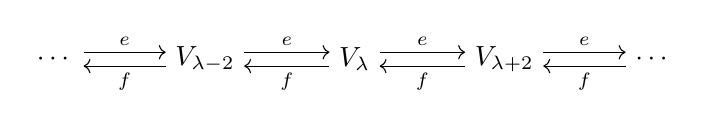
\begin{tikzpicture}[baseline=-3pt,x=1.9cm]
  \node (a) at (0,0) {$\cdots$};
  \node (b) at (1,0) {$V_{\lambda-2}$};
  \node (c) at (2,0) {$V_\lambda$};
  \node (d) at (3,0) {$V_{\lambda+2}$};
  \node (z) at (4,0) {$\cdots$};
  \foreach \x/\y in {a/b,b/c,c/d,d/z} {
    \draw[->] ([yshift=2.5pt]\x.east) -- node[above=-1pt]{\scriptsize $e$} ([yshift=2.5pt]\y.west);
    \draw[<-] ([yshift=-2.5pt]\x.east) -- node[below=-1pt]{\scriptsize $f$} ([yshift=-2.5pt]\y.west);
  }
\end{tikzpicture}
\]
E.g., in $L(n)$ we had $x^iy^j$ sitting in the place of the $V_\lambda$'s, and
the chain went from $\lambda = n$ to $\lambda = -n$:
\[
\begin{array}{*{13}{c}}
  V_n & \longleftrightarrow & V_{n-2} & \longleftrightarrow & V_{n-4} &
  \longleftrightarrow & \cdots & \longleftrightarrow & V_{-(n-4)} &
  \longleftrightarrow & V_{-(n-2)} & \longleftrightarrow & V_{-n}\\[2pt]
  \langle x^n\rangle & \rightleftarrows & \langle x^{n-1}y\rangle &
  \rightleftarrows & \langle x^{n-2}y^2\rangle & \rightleftarrows & \cdots &
  \rightleftarrows & \langle x^2y^{n-2}\rangle & \rightleftarrows &
  \langle xy^{n-1}\rangle & \rightleftarrows & \langle y^n\rangle
\end{array}
\]
(Note that the string for $L(n)$ has $n + 1$ elements.)

\begin{definition}
If $v \in V_\lambda \cap \ker e$, i.e.\ $hv = \lambda v$ and $ev = 0$, then we
say that $v$ is a \emph{highest-weight vector} of weight $\lambda$.
\end{definition}

\begin{lemma}
Let $V$ be a representation of $\sl_2$ and $v \in V$ a highest-weight vector
of weight $\lambda$. Then $W = \langle v, fv, f^2v, \dots\rangle$ is an
$\sl_2$-invariant subspace, i.e.\ a subrepresentation.
\end{lemma}

\begin{proof}
We need to show $hW \subseteq W$, $fW \subseteq W$, and $eW \subseteq W$.
Note that $fW \subseteq W$ by construction. Further, since $v \in V_\lambda$,
we saw above that $f^kv \in V_{\lambda - 2k}$, and so $hW \subseteq W$ as well.
Finally,
\begin{align*}
  ev &= 0 && \in W\\
  efv &= ([e, f] + fe)v = hv + f(0) = \lambda v && \in W\\
  ef^2v &= ([e, f] + fe)fv = (\lambda - 2)fv + f(\lambda v) = (2\lambda - 2)fv && \in W\\
  ef^3v &= ([e, f] + fe)f^2v = (\lambda - 4)f^2v + f(2\lambda - 2)fv = (3\lambda - 6)f^2v && \in W
\end{align*}
and so on.
\end{proof}

\begin{exercise}
$ef^nv = n(\lambda - n + 1)f^{n-1}v$ for $v$ a highest-weight vector of weight
$\lambda$.
\end{exercise}

\begin{lemma}
Let $V$ be a finite-dimensional representation of $\sl_2$ and $v \in V$ a
highest-weight vector of weight $\lambda$. Then $\lambda \in \Z_{\geq 0}$.
\end{lemma}

\begin{remark}
Somehow, the integrality condition is the Lie algebra remembering something
about the topology of the group. (Saying what this ``something'' is more
precisely is difficult.)
\end{remark}

\begin{proof}
Note that the $f^kv$ all lie in different eigenspaces of $h$, so if they are
all nonzero then they are linearly independent. Since $\dim V < \infty$, we
conclude that there exists a $k$ such that $f^kv \neq 0$ and $f^{k+r}v = 0$ for
all $r \geq 1$. Then by the above exercise,
\[
  0 = ef^{k+1}v = (k + 1)(\lambda - k)f^kv,
\]
from which $\lambda = k$, a nonnegative integer.
\end{proof}

\begin{proposition}
If $V$ is a nonzero finite-dimensional representation of $\sl_2$, it has a
highest-weight vector.
\end{proposition}

\begin{proof}
We're over $\C$, so we can pick some eigenvector $v$ of $h$, of eigenvalue
$\lambda$ say. Now apply $e$ to it repeatedly: $v, ev, e^2v, \dots$ belong to
different eigenspaces of $h$, so if they are nonzero, they are linearly
independent. Therefore, there must be some $k$ such that $e^kv \neq 0$ but
$e^{k+r}v = 0$ for all $r \geq 1$. Then $e^kv$ is a highest-weight vector of
weight $\lambda + 2k$.
\end{proof}

\begin{corollary}
If $V$ is an irreducible representation of $\sl_2$ then $\dim V = n + 1$ for
some $n \geq 0$, and $V$ has a basis $v_0, v_1, \dots, v_n$ on which $\sl_2$
acts as $hv_i = (n - 2i)v_i$; $fv_i = v_{i+1}$ (with $fv_n = 0$); and
$ev_i = i(n - i + 1)v_{i-1}$. In particular, there exists a unique
$(n+1)$-dimensional irreducible representation, which must be isomorphic to
$L(n)$.
\end{corollary}

\begin{exercise}
Work out how this basis is related to the basis we previously had for $L(n)$.
\end{exercise}

\lecture{4} We will now show that every finite-dimensional representation of
$\sl_2(\C)$ is a direct sum of irreducible representations, or
(equivalently) the category of finite-dimensional representations of
$\sl_2(\C)$ is \emph{semisimple}, or (equivalently) every representation of
$\sl_2(\C)$ is \emph{completely reducible}.

Morally, we've shown that every such representation consists of ``strings''
descending from the highest weight, and we'll now show that these strings
don't interact. We'll first show that they don't interact when they have
different highest weights (easier) and then that they also don't interact when
they have the same highest weight (harder).

We will also show that $h$ acts diagonalisably on every finite-dimensional
representation, while $e$ and $f$ are nilpotent. In fact,

\begin{remark}
\[
  \C h = \Bigl\{ \begin{pmatrix} a & \\ & -a \end{pmatrix} \Bigr\}
       = \Lie \Bigl\{ \begin{pmatrix} t & \\ & t^{-1} \end{pmatrix} \Bigr\}
       \subset \Lie(SL_2),
\]
where $\bigl\{\bigl(\begin{smallmatrix} t & \\ & t^{-1}\end{smallmatrix}\bigr)\bigr\}$
is the maximal torus inside $SL_2$. As for $\C^\times$, the representations
here should correspond to integers. In some hazy way, the fact that we are
picking out the representations of a circle and not any other $1$-dimensional
Lie group is a sign of the Lie algebra remembering something about the group.
(Saying what it is remembering and how is a hard question.)
\end{remark}

\begin{example}
Recall that $\C[x, y]$ is a representation of $\sl_2$ via the action by
differential operators, and is a direct sum of the representations $L(n)$.
\end{example}

\begin{exercise}
Show that the formulae $e = x\frac{\partial}{\partial y}$,
$f = y\frac{\partial}{\partial x}$,
$h = x\frac{\partial}{\partial x} - y\frac{\partial}{\partial y}$ give a
representation of $\sl_2$ on $x^\lambda y^\mu\C[x/y, y/x]$ for any
$\lambda, \mu \in \C$, and describe the submodule structure.
\end{exercise}

\begin{definition}
Let $V$ be a finite-dimensional representation of $\sl_2$. Define
$\Omega = ef + fe + \frac12 h^2 \in \End(V)$ to be the \emph{Casimir} of
$\sl_2$.
\end{definition}

\begin{lemma}
$\Omega$ is central; that is, $e\Omega = \Omega e$, $f\Omega = \Omega f$, and
$h\Omega = \Omega h$.
\end{lemma}

\begin{exercise}
Prove it. For example,
\begin{align*}
  e\Omega = e\Bigl(ef + fe + \frac12 h^2\Bigr)
    &= e(ef - fe) + 2(efe) + \frac12(eh - he)h + \frac12 heh\\
    &= 2efe + \frac12 heh\\
    &= (fe - ef)e + 2efe + \frac12 h(he - eh) + \frac12 heh = \Omega e.
\end{align*}
\end{exercise}

Observe that we can write
$\Omega = (ef - fe) + 2fe + \frac12 h^2 = (\frac12 h^2 + h) + 2fe$. This will
be useful later.

\begin{corollary}
If $V$ is an irreducible representation of $\sl_2$, then $\Omega$ acts on $V$
by a scalar.
\end{corollary}

\begin{proof}
Schur's lemma.
\end{proof}

\begin{lemma}
Let $L(n)$ be the irreducible representation of $\sl_2$ with highest weight
$n$. Then $\Omega$ acts on $L(n)$ by $\frac12 n^2 + n$.
\end{lemma}

\begin{proof}
It suffices to check this on the highest-weight vector $v$ (so $hv = nv$ and
$ev = 0$). Then
\[
  \Omega v = \Bigl(\frac12 h^2 + h + 2fe\Bigr)v = \Bigl(\frac12 n^2 + n\Bigr)v.
\]
Since $\Omega$ commutes with $f$ and $L(n)$ is spanned by the $f^iv$, we could
conclude directly (without using Schur's lemma) that $\Omega$ acts by this
scalar.
\end{proof}

Observe that if $L(n)$ and $L(m)$ are irreducible representations with
different highest weights, then $\Omega$ acts by different scalars on them
(since $\frac12 n(n + 2)$ is increasing in $n \geq 0$).

\begin{definition}
Let $V$ be a finite-dimensional representation of $\sl_2$. Set
\[
  V^\lambda = \setc{v \in V}{(\Omega - \lambda)^{\dim V}v = 0}.
\]
This is the \emph{generalised eigenspace of $\Omega$ with eigenvalue
$\lambda$}.
\end{definition}

\begin{claim}
Each $V^\lambda$ is a subrepresentation for $\sl_2$.
\end{claim}

\begin{proof}
Let $x \in \sl_2$ and $v \in V^\lambda$. Because $\Omega$ is central, we have
\[
  (\Omega - \lambda)^{\dim V}(xv) = x(\Omega - \lambda)^{\dim V}v = 0,
\]
so $xv \in V^\lambda$ as well.
\end{proof}

Now, if $V^\lambda \neq 0$, then $\lambda = \frac12 n^2 + n$, and $V^\lambda$
is somehow ``glued together'' from copies of $L(n)$. More precisely:

\begin{definition}
Let $W$ be a finite-dimensional $\g$-module. A \emph{composition series} for
$W$ is a sequence of submodules
\[
  0 = W_0 \subseteq W_1 \subseteq \dots \subseteq W_r = W
\]
such that each $W_i/W_{i-1}$ is an irreducible module.
\end{definition}

\begin{example}\leavevmode
\begin{enumerate}
  \item $\g = \C$, $W = \C^r$, where $1 \in \C$ acts as
    \[
      \begin{pmatrix}
        0 & 1 &        &        &   \\
          & 0 & 1      &        &   \\
          &   & \ddots & \ddots &   \\
          &   &        & \ddots & 1 \\
          &   &        &        & 0
      \end{pmatrix}.
    \]
    Then there exists a unique composition series for $W$, namely
    \[
      0 \subset \langle e_1\rangle \subset \langle e_1, e_2\rangle \subset \dots
        \subset \langle e_1, e_2, \dots, e_r\rangle.
    \]
  \item On the other hand, if $\g = \C$ and $W = \C^r$ with the zero action
    (i.e.\ $1 \in \C$ acts by $0$), then any chain
    $0 \subset W_1 \subset \dots \subset W_r$ with $\dim W_i = i$ will be a
    composition series.
\end{enumerate}
\end{example}

\begin{lemma}
Composition series always exist.
\end{lemma}

\begin{proof}
We induct on the dimension of $W$. Take a nonzero irreducible submodule
$W_1 \subseteq W$; then $W/W_1$ has smaller dimension, so has a composition
series. Taking its preimage in $W$ and sticking $W_1$ in front will do the
trick.
\end{proof}

\begin{remark}
The factors $W_i/W_{i-1}$ are determined by $W$ up to isomorphism and
reordering (the Jordan--H\"older theorem).
\end{remark}

So, the precise statement is that $V^\lambda$ has a composition series with
quotients $L(n)$ for some fixed $n$. Indeed, take an irreducible submodule
$L(n) \subset V^\lambda$; note that $\Omega$ acts on $L(n)$ by
$\frac12 n^2 + n$, so we must have $\lambda = \frac12 n^2 + n$, or in other
words $n$ is uniquely determined by $\lambda$; and moreover, $\Omega$ acts on
$V^\lambda/L(n)$, and its only generalised eigenvalue there is still
$\lambda$, so we can repeat the argument.

\begin{claim}
$h$ acts on $V^\lambda$ with generalised eigenvalues in the set
$\{n, n - 2, \dots, -n\}$.
\end{claim}

\begin{proof}
This is a general fact about composition series. Let $h$ act on $W$ and let
$W' \subset W$ be invariant under this action, i.e.\ $hW' \subseteq W'$. Then
\begin{multline*}
  \{\text{generalised eigenvalues of } h \text{ on } W\}
  = \{\text{generalised eigenvalues of } h \text{ on } W'\}\\
  \cup \{\text{generalised eigenvalues of } h \text{ on } W/W'\}.
\end{multline*}
(You can see this by looking at the block upper triangular form of the matrix
of $h$.) Now since $V^\lambda$ is composed of copies of $L(n)$, the generalised
eigenvalues of $h$ must lie in that set.
\end{proof}

Note also that on the kernel of $e\colon V^\lambda \to V^\lambda$ the only
generalised eigenvalue of $h$ is $n$; that is, $(h - n)^{\dim V^\lambda}x = 0$
for $x \in V^\lambda \cap \ker e$. (This follows by applying the above
observation to the composition series intersected with $\ker e$.)

\lecture{5}

\begin{lemma}\leavevmode
\begin{enumerate}
  \item $hf^k = f^k(h - 2k)$.
  \item $ef^{n+1} = f^{n+1}e + (n + 1)f^n(h - n)$.
\end{enumerate}
\end{lemma}

\begin{proof}
We saw (1) already, and (2) is the next exercise.
\end{proof}

\begin{exercise}
Prove (2) (by induction; e.g.\ for $n = 0$ the claim is $ef = fe + h$).
\end{exercise}

\begin{proposition}
$h$ acts diagonalisably on $\ker e\colon V^\lambda \to V^\lambda$; in fact, it
acts as multiplication by $n$. That is,
\[
  \ker\bigl(e\colon V^\lambda \to V^\lambda\bigr) = (V^\lambda)_n
    = \setc{x \in V^\lambda}{hx = nx}.
\]
\end{proposition}

Recall we know that $\ker e$ is (in) the \emph{generalised} eigenspace of $h$
with eigenvalue $n$ (and after the first line of the proof, we will have
equality rather than just containment). We are showing that we can drop the
word ``generalised''.

\begin{proof}
If $hx = nx$ then $ex \in (V^\lambda)_{n+2} = 0$ (as the generalised
eigenvalues of $h$ on $V^\lambda$ are $n, n - 2, \dots, -n$), so
$x \in \ker e$.

Conversely, let $x \in \ker e$; we know $(h - n)^{\dim V^\lambda}x = 0$. By
the lemma above,
\[
  (h - n + 2k)^{\dim V^\lambda}f^kx = f^k(h - n)^{\dim V^\lambda}x = 0.
\]
That is, $f^kx$ belongs to the generalised eigenspace of $h$ with eigenvalue
$n - 2k$.

On the other hand, for any $y \in \ker e$, $y \neq 0 \implies f^ny \neq 0$.

\begin{remark}
This should be an obvious property of upper-triangular matrices, but we'll
work it out in full detail.
\end{remark}

Take $0 = W_0 \subset W_1 \subset \dots \subset W_r = V^\lambda$, the
composition series for $V^\lambda$ with quotients $L(n)$. There is an $i$ such
that $y \in W_i$, $y \notin W_{i-1}$. Let
$\overline{y} = y + W_{i-1} \in W_i/W_{i-1} \cong L(n)$. Then $\overline{y}$ is
a highest-weight vector in $L(n)$, and so $f^n\overline{y} \neq 0$ in $L(n)$.
Therefore, $f^ny \neq 0$.

Now, $f^{n+1}x$ belongs to the generalised eigenspace of $h$ with eigenvalue
$-n - 2$, so is equal to $0$ (as the generalised eigenvalues of $h$ on
$V^\lambda$ are $n, n - 2, \dots, -n$). Therefore,
\[
  0 = ef^{n+1}x = (n + 1)f^n(h - n)x + f^{n+1}ex = (n + 1)f^n(h - n)x.
\]
Now, $(h - n)x \in \ker e$ (it's still in the generalised eigenspace of $h$
with eigenvalue $n$, and $e(h - n)x = (h - n - 2)ex = 0$), so if
$(h - n)x \neq 0$ then $f^n(h - n)x \neq 0$, and then
$(n + 1)f^n(h - n)x \neq 0$ in characteristic $0$, a contradiction. Therefore,
$hx = nx$.
\end{proof}

We can now finish the proof of complete reducibility. Indeed, choose a basis
$w_1, w_2, \dots, w_k$ of $\ker e\colon V^\lambda \to V^\lambda$, and consider
the ``string'' generated by each $w_i$; that is, consider
\[
  \langle w_i, fw_i, f^2w_i, \dots, f^nw_i\rangle.
\]

\begin{exercise}
Convince yourself that these strings constitute a direct sum decomposition of
$V^\lambda$; that is, these are subrepresentations, nonintersecting, linearly
independent, and span everything.
\end{exercise}

Therefore, $h$ acts semisimply and diagonalisably on $V^\lambda$, and
therefore on all of $V$.

\begin{exercise}
Show that this is false in characteristic $p$. That is, show that the
irreducible representations of $\sl_2(\Fpbar)$ are no longer parametrised by
$n \in \N$ (none of them has dimension greater than $p$), and find a
representation of $\sl_2(\Fpbar)$ that does not decompose into a direct sum of
irreducibles.
\end{exercise}

\section{Consequences}

Let $V, W$ be representations of a Lie algebra $\g$.

\begin{claim}
$\g \to \End(V \otimes W) = \End(V) \otimes \End(W)$ via
$x \mapsto x \otimes 1 + 1 \otimes x$ is a homomorphism of Lie algebras.
\end{claim}

\begin{exercise}
Prove it. (This comes from differentiating the group homomorphism
$G \to G \times G$ via $g \mapsto (g, g)$.)
\end{exercise}

\begin{corollary}
If $V, W$ are representations of $\g$, then so is $V \otimes W$.
\end{corollary}

\begin{remark}
If $A$ is an algebra and $V$ and $W$ are representations of $A$, then
$V \otimes W$ is naturally a representation of $A \otimes A$. To make it a
representation of $A$, we need an algebra homomorphism $A \to A \otimes A$.
(An object with such a structure, plus some other properties, is called a Hopf
algebra.) In some essential way, $\g$ behaves like a Hopf algebra. (Or,
rather, the universal enveloping algebra of $\g$ is a Hopf algebra, and so are
its deformations, the quantum groups.)
\end{remark}

Now, take $\g = \sl_2$. What is $L(n) \otimes L(m)$? That is, we know
$L(n) \otimes L(m) = \bigoplus_k a_kL(k)$; what are the $a_k$?

One method of doing this would be to compute all the highest-weight vectors.

\begin{exercise}
Do this for $L(1) \otimes L(n)$. Then do it for $L(2) \otimes L(n)$.
\end{exercise}

As a start on the exercise, let $v_a$ denote the highest-weight vector in
$L(a)$. Then $v_n \otimes v_m$ is a highest-weight vector in
$L(n) \otimes L(m)$. Indeed,
\begin{align*}
  h(v_n \otimes v_m) &= (hv_n) \otimes v_m + v_n \otimes (hv_m) = (n + m)\,v_n \otimes v_m,\\
  e(v_n \otimes v_m) &= (ev_n) \otimes v_m + v_n \otimes (ev_m) = 0 + 0 = 0.
\end{align*}
Therefore,
\[
  L(n) \otimes L(m) = L(n + m) + \text{other stuff}.
\]
However, counting dimensions, we get
\[
  (n + 1)(m + 1) = (n + m + 1) + \dim(\text{other stuff}),
\]
which shows that there is quite a lot of this ``other stuff'' in there.

One can write down explicit formulae for all the highest-weight vectors; these
are complicated but mildly interesting. However, we don't have to do it to
determine the summands of $L(n) \otimes L(m)$.

Let $V$ be a finite-dimensional representation of $\sl_2$.

\begin{definition}
The \emph{character} of $V$ is
$\ch V = \sum_{n \in \Z} \dim V_n\, z^n \in \N[z, z^{-1}]$.
\end{definition}

\begin{properties}\leavevmode
\begin{enumerate}
  \item $\ch V|_{z=1} = \dim V$.

    This is equivalent to the claim that $h$ is diagonalisable with
    eigenvalues in $\Z$, so $V = \bigoplus_{n \in \Z} V_n$.
  \item $\ch L(n) = z^n + z^{n-2} + \dots + z^{-n}
       = \dfrac{z^{n+1} - z^{-(n+1)}}{z - z^{-1}}$.
    Sometimes this is written as $[n + 1]_z$.
  \item $\ch V = \ch W$ iff $V \cong W$.

    Note that $\ch L(0) = 1$, $\ch L(1) = z + z^{-1}$,
    $\ch L(2) = z^2 + 1 + z^{-2}, \dots$ form a $\Z$-basis for the space of
    symmetric Laurent polynomials with integer coefficients. On the other
    hand, by complete reducibility,
    \begin{align*}
      V &= \textstyle\bigoplus_{n \geq 0} a_nL(n), \quad a_n \geq 0,\\
      W &= \textstyle\bigoplus_{n \geq 0} b_nL(n), \quad b_n \geq 0,\\
      V \cong W &\iff a_n = b_n \text{ for all } n.
    \end{align*}
    But since the $\ch L(n)$ form a basis, $\ch V = \sum a_n \ch L(n)$
    determines the $a_n$.

    \begin{remark}
    Note that for the representations, we only need nonnegative coefficients
    $a_n \geq 0$. On the other hand, if instead of looking at modules we were
    looking at chain complexes, the idea of $\Z$-linear combinations would
    become meaningful.
    \end{remark}
  \item $\ch(V \otimes W) = \ch V \cdot \ch W$.

    \begin{exercise}[Essential!]
    $V_n \otimes W_m \subseteq (V \otimes W)_{n+m}$. Therefore,
    $(V \otimes W)_p = \bigoplus_{n+m=p} V_n \otimes W_m$. This is exactly how
    we multiply polynomials.
    \end{exercise}

    \begin{example}
    We can now compute $L(1) \otimes L(3)$:
    \begin{align*}
      \ch L(1) \cdot \ch L(3) &= (z + z^{-1})(z^3 + z + z^{-1} + z^{-3})\\
        &= (z^4 + z^2 + 1 + z^{-2} + z^{-4}) + (z^2 + 1 + z^{-2})
         = \ch L(4) + \ch L(2),
    \end{align*}
    so $L(1) \otimes L(3) = L(4) \oplus L(2)$.
    \end{example}
  \item The Clebsch--Gordan rule:
    \[
      L(n) \otimes L(m) = \bigoplus_{\substack{k = |n - m|\\ k \equiv n - m \bmod 2}}^{n + m} L(k).
    \]
    There is a picture that goes with this rule (so you don't actually need to
    remember it); see figure~\ref{fig:crystal-sl2}.
\end{enumerate}
\end{properties}

\begin{figure}[!htbp]
  \centering
  \slcrystal
  \caption{Crystal for $\sl_2$, drawn for $n = 4$, $m = 6$.}
  \label{fig:crystal-sl2}
\end{figure}

The individual strings are the $L(a)$ in the decomposition.

One of the points of this course is that this sort of picture-drawing (called
crystals) lets us decompose tensor products of representations of all other
semisimple Lie algebras. (This fact was discovered about 20 years ago by
Kashiwara and Lusztig.)

What we will actually show for the other semisimple Lie algebras:
\begin{itemize}
  \item The category of finite-dimensional representations is completely
    reducible (i.e.\ all finite-dimensional representations are semisimple).
  \item We will parametrise the irreducible representations.
  \item We will compute the characters of the irreducible representations.
  \item We will show how to take tensor products of irreducible
    representations by drawing pictures (crystals).
\end{itemize}

\section{Structure and classification of simple Lie algebras}

\lecture{6} We begin with some linear algebra preliminaries.

\begin{definition}
A Lie algebra $\g$ is called \emph{simple} if the only ideals in $\g$ are $0$
and $\g$, and $\dim \g > 1$ (equivalently, given the first condition, $\g$ is
not abelian). A Lie algebra $\g$ is called \emph{semisimple} if it is a direct
sum of simple Lie algebras.
\end{definition}

\begin{remark}
Recall that $\C$ behaved quite differently from $\sl_2$, so it is sensible to
exclude the abelian Lie algebras.
\end{remark}

\begin{definition}
The \emph{derived algebra} of $\g$ is
$[\g, \g] = \Span\setc{[x, y]}{x, y \in \g}$.
\end{definition}

\begin{exercise}\leavevmode
\begin{enumerate}
  \item $[\g, \g]$ is an ideal;
  \item $\g/[\g, \g]$ is abelian.
\end{enumerate}
\end{exercise}

\begin{definition}
The \emph{central series} of $\g$ is given by $\g^0 = \g$,
$\g^n = [\g^{n-1}, \g]$, i.e.
\[
  \g \supseteq [\g, \g] \supseteq [[\g, \g], \g] \supseteq \cdots
\]
The \emph{derived series} of $\g$ is given by $\g^{(0)} = \g$,
$\g^{(n)} = [\g^{(n-1)}, \g^{(n-1)}]$, i.e.
\[
  \g \supseteq [\g, \g] \supseteq [[\g, \g], [\g, \g]] \supseteq \cdots
\]
\end{definition}

\begin{remark}
Clearly, $\g^{(n)} \subseteq \g^n$.
\end{remark}

\begin{definition}
$\g$ is \emph{nilpotent} if $\g^n = 0$ for some $n > 0$, i.e.\ the central
series terminates. $\g$ is \emph{solvable} if $\g^{(n)} = 0$ for some $n > 0$,
i.e.\ the derived series terminates.
\end{definition}

By the above remark, a nilpotent Lie algebra is necessarily solvable.

\begin{remark}
The term ``solvable'' comes from Galois theory (if the Galois group is
solvable, the associated polynomial is solvable by radicals). We will see
shortly where the term ``nilpotent'' comes from.
\end{remark}

\begin{example}\leavevmode
\begin{enumerate}
  \item $\fn = \Biggl\{ \begin{pmatrix}
            0 & * & \cdots & *\\
              & 0 & \cdots & *\\
              &   & \ddots & \vdots\\
              &   &        & 0
          \end{pmatrix} \in \gl_n \Biggr\}$, the strictly upper triangular
    matrices, form a nilpotent Lie algebra.
  \item $\fb = \Biggl\{ \begin{pmatrix}
            * & * & \cdots & *\\
              & * & \cdots & *\\
              &   & \ddots & \vdots\\
              &   &        & *
          \end{pmatrix} \in \gl_n \Biggr\}$, the upper triangular matrices,
    form a solvable Lie algebra.

    \begin{exercise}[Essential]\leavevmode
    \begin{alist}
      \item Compute the central and derived series to check that these
        algebras are nilpotent and solvable respectively.
      \item Compute the centre of these algebras.
    \end{alist}
    \end{exercise}
  \item Let $W$ be a symplectic vector space with inner product
    $\langle\,,\,\rangle$ (recall that a symplectic vector space is equipped
    with a nondegenerate bilinear antisymmetric form, and there is essentially
    one example: given a finite-dimensional vector space $L$ let
    $W = L + L^*$ with inner product
    $\langle L, L\rangle = \langle L^*, L^*\rangle = 0$ and
    $\langle v, v^*\rangle = -\langle v^*, v\rangle = v^*(v)$). Define the
    \emph{Heisenberg Lie algebra} as
    \[
      \Heis_W = W \oplus \C c, \qquad [w, w'] = \langle w, w'\rangle c, \quad [c, w] = 0.
    \]

    \begin{exercise}
    Show this is a Lie algebra, and that it is nilpotent.
    \end{exercise}

    This is the most important nilpotent Lie algebra occurring in nature. For
    example, let $L = \C$; then $\Heis_W = \C p + \C q + \C c$ with
    $[p, q] = c$, $[p, c] = [q, c] = 0$ (as we know from classifying the
    $3$-dimensional Lie algebras!). Show that this has a representation on
    $\C[x]$ via $q \mapsto$ multiplication by $x$, $p \mapsto \partial/\partial x$,
    $c \mapsto 1$.

    (For a general vector space $L$, the basis vectors $v_1, \dots, v_n$ map
    to multiplication by $x_1, \dots, x_n$, and their duals map to
    $\partial/\partial x_1, \dots, \partial/\partial x_n$.)
\end{enumerate}
\end{example}

\begin{properties}\leavevmode
\begin{enumerate}
  \item Subalgebras and quotients of solvable Lie algebras are solvable.
    Subalgebras and quotients of nilpotent Lie algebras are nilpotent.
  \item Let $\g$ be a Lie algebra, and let $\h$ be an ideal of $\g$. Then $\g$
    is solvable if and only if $\h$ and $\g/\h$ are both solvable. (That is,
    solvable Lie algebras are built out of abelian Lie algebras, i.e.\ there
    is a refinement of the derived series such that the subquotients are
    $1$-dimensional and therefore abelian.)
  \item A nonzero $\g$ is nilpotent iff the centre of $\g$ is nonzero and
    $\g/(\text{centre of } \g)$ is nilpotent. Indeed, if $\g$ is nilpotent,
    then the central series is
    \[
      \g \supsetneq \g^1 \supsetneq \cdots \supsetneq \g^{n-1} \supsetneq \g^n = 0,
    \]
    and since $\g^n = [\g^{n-1}, \g]$ we must have $\g^{n-1}$ contained in the
    centre of $\g$.
  \item $\g$ is nilpotent iff $\ad \g \subseteq \gl(\g)$ is nilpotent, as we
    have an exact sequence
    \[
      0 \to \text{centre of } \g \hookrightarrow \g \twoheadrightarrow \ad \g \to 0.
    \]
\end{enumerate}
\end{properties}

\begin{exercise}
Prove the properties. (The proofs should all be easy and tedious.)
\end{exercise}

We now state a nontrivial result, which we will not prove.

\begin{theorem}[Lie's theorem]
Let $\g \subseteq \gl(V)$ be a solvable Lie algebra, where $V \neq 0$ is
finite-dimensional, and let the base field $k$ be algebraically closed and
have characteristic zero. Then there exists a basis $v_1, \dots, v_n$ of $V$
with respect to which $\g \subseteq \fb(V)$, i.e.\ the matrices of all elements
of $\g$ are upper triangular.

Equivalently, there exist a linear function $\lambda\colon \g \to k$ and a
nonzero $v \in V$ such that $xv = \lambda(x)v$ for all $x \in \g$, i.e.\ $v$ is
a common eigenvector for all of $\g$, i.e.\ $kv$ is a one-dimensional
subrepresentation.
\end{theorem}

In particular, the only irreducible finite-dimensional representations of a
solvable $\g$ are one-dimensional.

\begin{exercise}
Show that these are actually equivalent. (One direction should be obvious; in
the other, quotient by $v_1$ and repeat.)
\end{exercise}

\begin{exercise}
Show that we need $k$ to be algebraically closed.

Show that we need $k$ to have characteristic $0$. [\emph{Hint:} let $\g$ be
the $3$-dimensional Heisenberg Lie algebra, and show that $k[x]/x^p$ is a
finite-dimensional irreducible representation of dimension markedly bigger
than $1$.]
\end{exercise}

\begin{corollary}
In characteristic $0$, if $\g$ is a solvable finite-dimensional Lie algebra,
then $[\g, \g]$ is nilpotent.
\end{corollary}

\begin{exercise}
Find a counterexample in characteristic $p$.
\end{exercise}

\begin{proof}
Apply Lie's theorem to the adjoint representation $\g \to \End(\g)$. With
respect to some basis, $\ad \g \subseteq \fb(\g)$. Since $[\fb, \fb] \subseteq \fn$
(note the diagonal entries cancel out when we take the bracket), we see that
$[\ad \g, \ad \g]$ is nilpotent. Since $\ad[\g, \g] = [\ad \g, \ad \g]$ (it's a
representation!), we see that $\ad[\g, \g]$ is nilpotent, and therefore so is
$[\g, \g]$.
\end{proof}

\begin{theorem}[Engel's theorem]
Let the base field $k$ be arbitrary, and let $\g$ be finite-dimensional. Then
$\g$ is nilpotent iff $\ad \g$ consists of nilpotent endomorphisms of $\g$
(i.e., for all $x \in \g$, $\ad x$ is nilpotent).

Equivalently, if $V \neq 0$ is a finite-dimensional representation of $\g$ such
that all elements of $\g$ act on $V$ by nilpotent endomorphisms, then there
exists a nonzero $v \in V$ such that $x(v) = 0$ for all $x \in \g$, i.e.\ $V$
has the trivial representation as a subrepresentation.

Equivalently, in a suitable basis every $x \in \g$ acts by a strictly upper
triangular matrix.
\end{theorem}

\begin{exercise}
Show that these are actually equivalent.
\end{exercise}

\lecture{7}

\begin{definition}
A symmetric bilinear form $(\,,\,)\colon \g \times \g \to k$ is
\emph{invariant} if $([x, y], z) = (x, [y, z])$.
\end{definition}

\begin{exercise}
If $\fa \subseteq \g$ is an ideal and $(\,,\,)$ is an invariant bilinear form,
then $\fa^\perp$ is an ideal.
\end{exercise}

\begin{definition}
If $V$ is a finite-dimensional representation of $\g$, i.e.\ if
$\rho\colon \g \to \gl(V)$ is a homomorphism, define the \emph{trace form} to
be $(x, y)_V = \tr\bigl(\rho(x)\rho(y)\colon V \to V\bigr)$.
\end{definition}

\begin{exercise}
Check that the trace form is symmetric, bilinear, and invariant. (They should
all be obvious.)
\end{exercise}

\begin{example}
$(\,,\,)_{\ad}$ is the ``Killing form'' (named after a person, not after an
action). This is the trace form attached to the adjoint representation. That
is, $(x, y)_{\ad} = \tr(\ad x \ad y\colon \g \to \g)$.
\end{example}

\begin{theorem}[Cartan's criterion]
Let $\g \subseteq \gl(V)$ and let $\charac k = 0$. Then $\g$ is solvable if and
only if $(x, y)_V = 0$ for every $x \in \g$ and $y \in [\g, \g]$. (That is,
$[\g, \g] \subseteq \g^\perp$.)
\end{theorem}

\begin{exercise}
Lie's theorem gives us one direction. Indeed, if $\g$ is solvable then we can
take a basis in which $x$ is an upper triangular matrix, $y$ is strictly upper
triangular, and then $xy$ and $yx$ both have zeros on the diagonal (and thus
trace $0$). That is, if $\g$ is solvable and nonabelian, all trace forms are
degenerate. (The exercise is to convince yourself that this is true.)
\end{exercise}

\begin{corollary}
$\g$ is solvable iff $(\g, [\g, \g])_{\ad} = 0$.
\end{corollary}

\begin{proof}
If $\g$ is solvable, Lie's theorem gives the trace to be zero. Conversely,
Cartan's criterion tells us that $\ad \g = \g/(\text{centre of } \g)$ is
solvable, and therefore so is $\g$.
\end{proof}

\begin{exercise}
Not every invariant form is a trace form. Let
$\tilde\Heis = \C\langle p, q, c, d\rangle$ where $[c, \tilde\Heis] = 0$,
$[p, q] = c$, $[d, p] = p$, $[d, q] = -q$.
\begin{enumerate}
  \item Construct a nondegenerate invariant form on $\tilde\Heis$.
  \item Show $\tilde\Heis$ is solvable.
  \item Extend the representation of $\langle c, p, q\rangle = \Heis$ on
    $k[x]$ to a representation of $\tilde\Heis$.
\end{enumerate}
\end{exercise}

\begin{definition}
The \emph{radical} of $\g$, $R(\g)$, is the maximal solvable ideal in $\g$.
\end{definition}

\begin{exercise}\leavevmode
\begin{enumerate}
  \item Show $R(\g)$ is the sum of all solvable ideals in $\g$ (i.e., show
    that the sum of solvable ideals is solvable).
  \item Show $R(\g/R(\g)) = 0$.
\end{enumerate}
\end{exercise}

\begin{theorem}
In characteristic $0$, the following are equivalent:
\begin{enumerate}
  \item $\g$ is semisimple;
  \item $R(\g) = 0$;
  \item the Killing form $(\,,\,)_{\ad}$ is nondegenerate (the Killing
    criterion).
\end{enumerate}
Moreover, if $\g$ is semisimple, then every derivation $D\colon \g \to \g$ is
inner, but not conversely (where we define the terms ``derivation'' and
``inner'' below).
\end{theorem}

\begin{definition}
A \emph{derivation} $D\colon \g \to \g$ is a linear map satisfying
$D[x, y] = [Dx, y] + [x, Dy]$.
\end{definition}

\begin{example}
$\ad(x)$ is a derivation for any $x$. Derivations of the form $\ad(x)$ for some
$x \in \g$ are called \emph{inner}.
\end{example}

\begin{remark}
If $\g$ is any Lie algebra, we have the exact sequence
\[
  0 \to R(\g) \hookrightarrow \g \twoheadrightarrow \g/R(\g) \to 0,
\]
where $R(\g)$ is a solvable ideal, and $\g/R(\g)$ is semisimple. That is, any
Lie algebra has a maximal semisimple quotient, and the kernel is a solvable
ideal. This shows you how much nicer the theory of Lie algebras is than the
corresponding theory for finite groups. In particular, the corresponding
statement for finite groups is essentially equivalent to the classification of
the finite simple groups.
\end{remark}

A theorem that we will neither prove nor use, but which is pretty:

\begin{theorem}[Levi's theorem]
In characteristic $0$, a stronger result is true. Namely, the exact sequence
splits, i.e.\ there exists a subalgebra $\fs \subseteq \g$ such that
$\fs \cong \g/R(\g)$. (This subalgebra is not canonical; in particular, it is
not an ideal of $\g$.) That is, $\g$ can be written as
$\g = \fs \ltimes R(\g)$.
\end{theorem}

\begin{exercise}
Show that this fails in characteristic $p$. Let $\g = \sl_p(\Fpbar)$; show
$R(\g) = \Fpbar I$ (note that the identity matrix in dimension $p$ has trace
$0$), but that there is no complement to $R(\g)$ that is an algebra.
\end{exercise}

\begin{proof}[Proof of Theorem~4.7]
First, notice that $R(\g) = 0$ if and only if $\g$ has no nonzero abelian
ideals. (In one direction, an abelian ideal is solvable; in the other, notice
that the last nonzero term of the derived series of $R(\g)$ is an abelian
ideal of $\g$.)

From now on, $(\,,\,)$ refers to the Killing form $(\,,\,)_{\ad}$.

(3) $\implies$ (2): we show that if $\fa$ is an abelian ideal of $\g$, then
$\fa \subseteq \g^\perp$. (Since the Killing form is nondegenerate, this means
$\fa = 0$, and therefore $R(\g) = 0$.)

Write $\g = \fa + \h$ where $\h$ is a vector space complement to $\fa$ (not
necessarily an ideal). For $a \in \fa$, $\ad a$ has block matrix
$\bigl(\begin{smallmatrix} 0 & * \\ 0 & 0 \end{smallmatrix}\bigr)$. For
$x \in \g$, $\ad x$ has block matrix
$\bigl(\begin{smallmatrix} * & * \\ 0 & * \end{smallmatrix}\bigr)$. (This is
because $\fa$ is an ideal, so $[a, x] \in \fa$ for all $x \in \g$, and moreover
$\ad a$ acts by $0$ on $\fa$.) Therefore,
\[
  \tr(\ad a \cdot \ad x) = \tr \begin{pmatrix} 0 & * \\ 0 & 0 \end{pmatrix} = 0,
\]
i.e.\ $(\fa, \g)_{\ad} = 0$. Since the Killing form is nondegenerate, $\fa = 0$.

(2) $\implies$ (3): Let $\fr \subseteq \g^\perp$ be an ideal (e.g.\
$\fr = \g^\perp$), and suppose $\fr \neq 0$. Then $\ad \fr \subseteq \gl(\g)$,
and $(x, y)_{\ad} = 0$ for all $x, y \in \fr$. By Cartan's criterion,
$\ad \fr \cong \fr/(\fr \cap \text{centre of } \g)$ is solvable, so $\fr$ is
solvable, contradicting $R(\g) = 0$.

\begin{exercise}
Show that $R(\g) \supseteq \g^\perp \supseteq [R(\g), R(\g)]$.
\end{exercise}

(2), (3) $\implies$ (1): Let $(\,,\,)_{\ad}$ be nondegenerate, and let
$\fa \subseteq \g$ be a minimal nonzero ideal. We claim that
$(\,,\,)_{\ad}|_{\fa}$ is either $0$ or nondegenerate. Indeed, the kernel of
$(\,,\,)_{\ad}|_{\fa}$ is
$\setc{x \in \fa}{(x, \fa)_{\ad} = 0} = \fa \cap \fa^\perp$, which is an ideal!

Cartan's criterion implies that $\fa$ is solvable if $(\,,\,)_{\ad}|_{\fa}$ is
$0$. Since $R(\g) = 0$, we conclude that $(\,,\,)_{\ad}|_{\fa}$ is
nondegenerate.

Therefore, $\g = \fa \oplus \fa^\perp$, where $\fa$ is a minimal ideal, i.e.\
simple. (Note that $R(\g) = 0$, so $\fa$ cannot be abelian.)

But now ideals of $\fa^\perp$ are ideals of $\g$, so we can apply the same
argument to $\fa^\perp$, since $R(\g) = 0 \implies R(\fa^\perp) = 0$.
Therefore, $\g = \bigoplus \fa_i$, where the $\fa_i$ are simple Lie algebras.
\end{proof}

\begin{exercise}
Show that if $\g$ is semisimple, then $\g$ is the direct sum of minimal ideals
\emph{in a unique manner}. That is, if $\g = \bigoplus \fa_i$ where the
$\fa_i$ are minimal, and $\fb$ is a minimal ideal of $\g$, then in fact
$\fb = \fa_i$ for some $i$. (Consider $\fb \cap \fa_j$.) Conclude that
(1) $\implies$ (2).
\end{exercise}

\lecture{8} Finally, we show that all derivations on semisimple Lie algebras
are inner. Let $\g$ be a semisimple Lie algebra, and let $D\colon \g \to \g$ be
a derivation. Consider the linear functional $l\colon \g \to k$ via
$x \mapsto \tr(D \cdot \ad x)$. Since $\g$ is semisimple, the Killing form is a
nondegenerate inner product giving an isomorphism with the dual, so there
exists $y \in \g$ such that $l(x) = (y, x)_{\ad}$. Our task is to show that
$D = \ad y$, i.e.\ that $E := D - \ad y = 0$.

This is equivalent to showing that $Ex = 0$ for all $x \in \g$, or
equivalently that $(Ex, z)_{\ad} = 0$ for all $z \in \g$. Now,
\[
  \ad(Ex) = E \cdot \ad x - \ad x \cdot E = [E, \ad x]\colon \g \to \g,
\]
since $\ad(Ex)(z) = [Ex, z] = E[x, z] - [x, Ez]$. Therefore,
\begin{align*}
  (Ex, z)_{\ad} &= \tr_\g(\ad(Ex) \cdot \ad z) = \tr_\g([E, \ad x] \cdot \ad z)\\
    &= \tr_\g(E \cdot [\ad x, \ad z]) = \tr_\g(E \cdot \ad[x, z]).
\end{align*}
But by definition of $E$, for any $a \in \g$ (here $a = [x, z]$),
$\tr_\g(E \cdot \ad a) = \tr_\g(D \cdot \ad a) - (y, a)_{\ad} = l(a) - l(a) = 0$.
\qed

\begin{exercise}\leavevmode
\begin{enumerate}
  \item A nonzero nilpotent Lie algebra always has non-inner derivations.
  \item $\g = \langle a, b\rangle$ with $[a, b] = b$ only has inner
    derivations. Thus, this condition doesn't characterise semisimplicity.
\end{enumerate}
\end{exercise}

\begin{exercise}\leavevmode
\begin{enumerate}
  \item Let $\g$ be a simple Lie algebra, and $(\,,\,)_1$ and $(\,,\,)_2$ two
    non-degenerate invariant bilinear forms. Show that there exists $\lambda$
    such that $(\,,\,)_1 = \lambda(\,,\,)_2$.
  \item Let $\g = \sl_n(\C)$. We will shortly show that this is a simple Lie
    algebra. We have two nondegenerate bilinear forms: the Killing form
    $(\,,\,)_{\ad}$ and $(A, B) = \tr(AB)$ in the standard representation.
    Compute $\lambda$.
\end{enumerate}
\end{exercise}

\section{Structure theory}

\begin{definition}
A \emph{torus} $\at \subseteq \g$ is an abelian subalgebra such that for all
$t \in \at$ the adjoint $\ad(t)\colon \g \to \g$ is a diagonalisable linear
map. A \emph{maximal torus} is a torus that is not contained in any bigger
torus.
\end{definition}

\begin{example}
Let $T = (S^1)^r \subseteq G$ where $G$ is a compact Lie group (or
$T = (\C^\times)^r \subseteq G$ where $G$ is a reductive algebraic group). Then
$\at = \Lie(T) \subseteq \g = \Lie(G)$ is a torus, maximal if $T$ is. (This
comes from knowing that representations of $T$ are diagonalisable by an
averaging argument, but we don't really know this.)
\end{example}

\begin{exercise}\leavevmode
\begin{enumerate}
  \item For $\g = \sl_n$ or $\g = \gl_n$, the diagonal matrices (of trace $0$
    if inside $\sl_n$) form a maximal torus $\at$.
  \item $\bigl(\begin{smallmatrix} 0 & * \\ 0 & 0 \end{smallmatrix}\bigr)$ is
    \emph{not} a torus. (We should know this is not diagonalisable!)
\end{enumerate}
\end{exercise}

For a vector space $V$, let $t_1, \dots, t_r\colon V \to V$ be pairwise
commuting diagonalisable linear maps; let
$\lambda = (\lambda_1, \dots, \lambda_r) \in \C^r$. Set
$V_\lambda = \setc{v \in V}{t_iv = \lambda_iv \text{ for all } i}$, the
simultaneous eigenspace.

\begin{lemma}
$V = \bigoplus_{\lambda \in \C^r} V_\lambda$.
\end{lemma}

\begin{proof}
Induct on $r$. For $r = 1$ this follows from the requirement that $t_1$ be
diagonalisable. For $r > 1$, look at $t_1, \dots, t_{r-1}$ and decompose
\[
  V = \bigoplus V_{(\lambda_1, \dots, \lambda_{r-1})}.
\]
Since $t_r$ commutes with $t_1, \dots, t_{r-1}$, it preserves the
decomposition. Now decompose each $V_{(\lambda_1, \dots, \lambda_{r-1})}$ into
eigenspaces for $t_r$ (the restriction of a diagonalisable map to an invariant
subspace is diagonalisable).
\end{proof}

Let $\at$ be the $r$-dimensional abelian Lie algebra with basis
$(t_1, \dots, t_r)$. The lemma asserts that $V$ is a semisimple (i.e.\
completely reducible) representation of $\at$. $V = \bigoplus V_\lambda$ is the
decomposition into isotypic representations. Namely, letting $\C_\lambda$ be
the $1$-dimensional representation wherein $t_i(w) = \lambda_iw$, we have
$\lambda \neq \mu \implies \C_\lambda \not\cong \C_\mu$, and $V_\lambda$ is
the direct sum of $\dim V_\lambda$ copies of $\C_\lambda$.

\begin{exercise}
Show that every irreducible representation of $\at$ is one-dimensional.
\end{exercise}

Another way of saying this is as follows. $\lambda$ is a linear map
$\at \to \C$, i.e.\ an element of the dual space $\lambda \in \at^*$ (sending
$t_i \mapsto \lambda_i$). Therefore, one-dimensional representations of $\at$
(which are all the irreducible representations of $\at$) correspond to
elements of $\at^* = \Hom_{\text{vector spaces}}(\at, \C)$. The decomposition
\[
  V = \bigoplus_{\lambda \in \at^*} V_\lambda, \qquad
  V_\lambda = \setc{v \in V}{t(v) = \lambda(t)v \text{ for all } t \in \at}
\]
is called the \emph{weight space decomposition} of $V$.

Now, let $\g$ be a Lie algebra and $\at$ a maximal torus. The weight space
decomposition of $\g$ is
\[
  \g = \g_0 \oplus \bigoplus_{\substack{\lambda \in \at^*\\ \lambda \neq 0}} \g_\lambda,
\]
where $\g_0 = \setc{x \in \g}{[t, x] = 0 \text{ for all } t \in \at}$ and
$\g_\lambda = \setc{x \in \g}{[t, x] = \lambda(t)x \text{ for all } t \in \at}$.

\begin{definition}
$R = \setc{\lambda \in \at^*}{\g_\lambda \neq 0,\ \lambda \neq 0}$ is the set
of \emph{roots} of $\g$.
\end{definition}

We will now compute the root space decomposition for $\sl_n$.

\begin{example}
$\g = \sl_n$, $\at = $ diagonal matrices in $\sl_n$. Let
\[
  t = \begin{pmatrix} t_1 & & 0 \\ & \ddots & \\ 0 & & t_n \end{pmatrix}
\]
and let $E_{ij}$ be the matrix with $1$ in the $(i, j)$th position and $0$
elsewhere. Then $[t, E_{ij}] = (t_i - t_j)E_{ij}$.

Let $\eps_i \in \at^*$, $\eps_i(t) = t_i$. Then $\eps_1, \dots, \eps_n$ span
$\at^*$, but $\eps_1 + \dots + \eps_n = 0$.

\begin{remark}
$\at$ is a subalgebra of $\C^n$, so $\at^*$ should be a quotient of
$(\C^n)^*$, and here is the relation by which it is a quotient.
\end{remark}

Therefore, we can rewrite the above as
$[t, E_{ij}] = (\eps_i - \eps_j)(t) \cdot E_{ij}$. Therefore, the roots are
$R = \setc{\eps_i - \eps_j}{i \neq j}$ and $\g_0 = \at$. (Note that we've shown
$\at$ is a maximal torus in the process.) The root space
$\g_{\eps_i - \eps_j} = \C E_{ij}$ is one-dimensional.

That is, the root space decomposition of $\sl_n$ is
\[
  \sl_n = \at \oplus \bigoplus_{\eps_i - \eps_j \in R} \g_{\eps_i - \eps_j}.
\]
\end{example}

\begin{exercise}
``This is (a) an essential exercise, and (b) guaranteed to be on the exam. The
first should get you to do it, the second is irrelevant.''

Compute the root space decomposition for $\sl_n$ (as we just did),
$\so_{2n}$, $\so_{2n+1}$, $\spl_{2n}$, where $\at$ is the diagonal matrices
in $\g$, and we take the conjugate $\so_n$ defined by
\[
  \so_n = \setc{A \in \gl_n}{JA + A^TJ = 0}, \qquad
  J = \begin{pmatrix} 0 & & 1 \\ & \iddots & \\ 1 & & 0 \end{pmatrix}
\]
(this is conjugate to the usual $\so_n$ since we've defined a nondegenerate
inner product; in this version, the diagonal matrices are a maximal torus).
The symplectic matrices are given by the same embedding as before.

In particular, show that $\at$ is a maximal torus and the root spaces are
one-dimensional.
\end{exercise}

\lecture{9} The Lie algebras we were working with last time are called the
``classical'' Lie algebras (they are Lie algebras of automorphisms of vector
spaces preserving a form). The rest of the course will be concerned with
explaining how their roots control their representations.

\begin{proposition}
$\sl_n(\C)$ is simple.
\end{proposition}

\begin{proof}
Recall
\[
  \sl_n(\C) = \at \oplus \bigoplus_{\alpha \in R} \g_\alpha,
\]
where $R = \setc{\eps_i - \eps_j}{i \neq j}$ and $\g_{\eps_i - \eps_j} = \C E_{ij}$.

Suppose $\fr \subseteq \sl_n$ is a nonzero ideal. Choose $r \in \fr$,
$r \neq 0$, such that when we write $r = t + \sum_{\alpha \in R} e_\alpha$
with $t \in \at$ and $e_\alpha \in \g_\alpha$, the number of nonzero terms is
minimal.

First, suppose $t \neq 0$. Choose $t_0 \in \at$ such that $\alpha(t_0) \neq 0$
for all $\alpha \in R$ (i.e., $t_0$ has distinct eigenvalues). Consider
$[t_0, r] = \sum_{\alpha \in R} \alpha(t_0)e_\alpha$. Note that this lies in
$\fr$, and if it is nonzero, it has fewer nonzero terms than $r$, a
contradiction. Thus, $[t_0, r] = 0$, i.e.\ $r = t \in \at$.

Since $t \neq 0$, there exists $\alpha = \eps_i - \eps_j \in R$ with
$\alpha(t) \neq 0$ (i.e.\ $t$ can't have all its eigenvalues equal, since it
has trace $0$). Then
\[
  [t, E_{ij}] = \alpha(t)E_{ij} \in \fr \implies E_{ij} \in \fr.
\]
Now,
\[
  [E_{ij}, E_{jk}] = E_{ik} \text{ for } i \neq k, \qquad
  [E_{si}, E_{ij}] = E_{sj} \text{ for } s \neq j,
\]
and therefore $E_{ab} \in \fr$ for all $a \neq b$. Finally,
\[
  [E_{i,i+1}, E_{i+1,i}] = E_{ii} - E_{i+1,i+1} \in \fr,
\]
so in fact the entire basis for $\sl_n$ lies in $\fr$ and $\fr = \sl_n$.

\begin{remark}
This is actually a combinatorial statement about root spaces; we'll see more
about this later.
\end{remark}

That leaves us with the case $t = 0$. If $r = cE_{ij}$ has only one nonzero
term, we are done exactly as above; therefore,
\[
  r = e_\alpha + e_\beta + \sum_{\gamma \in R - \{\alpha, \beta\}} e_\gamma,
  \qquad \alpha \neq \beta,\ e_\alpha, e_\beta \neq 0.
\]
Choose $t_0 \in \at$ such that $\alpha(t_0) \neq \beta(t_0)$; then
$[t_0, r] - \beta(t_0)r$ is nonzero and has fewer nonzero terms than $r$, a
contradiction.
\end{proof}

\begin{proposition}
Let $\g$ be a semisimple Lie algebra. Then maximal tori exist (i.e.\ are
nonzero). Moreover,
$\g_0 = \setc{x \in \g}{[\at, x] = 0} = \at$. (Recall that $\at$ is not defined
to be the maximal abelian subalgebra, but as the maximal abelian subalgebra
whose adjoint acts semisimply.)
\end{proposition}

We won't prove this; the proof involves introducing the Cartan subalgebra and
showing that it's the same as a maximal torus. As a result, we will sometimes
be calling $\at$ the Cartan subalgebra.

This means that the root space decomposition of a semisimple Lie algebra is
\[
  \g = \at \oplus \bigoplus_{\alpha \in R} \g_\alpha,
\]
as we have, of course, already seen for the classical Lie algebras.

\begin{theorem}[Structure theorem for semisimple Lie algebras, part I]
Let $\g$ be a semisimple Lie algebra over $\C$, and let $\at \subseteq \g$ be a
maximal torus. Write $\g = \at \oplus \bigoplus_{\alpha \in R} \g_\alpha$. Then
\begin{enumerate}
  \item $\C R = \at^*$, i.e.\ the roots span $\at^*$.
  \item $\dim \g_\alpha = 1$.
  \item If $\alpha, \beta \in R$ and $\alpha + \beta \in R$ then
    $[\g_\alpha, \g_\beta] = \g_{\alpha+\beta}$. If $\alpha + \beta \notin R$
    and $\alpha \neq -\beta$ then $[\g_\alpha, \g_\beta] = 0$.
  \item $[\g_\alpha, \g_{-\alpha}] \subseteq \at$ is one-dimensional, and
    $\g_\alpha \oplus [\g_\alpha, \g_{-\alpha}] \oplus \g_{-\alpha}$ is a Lie
    subalgebra of $\g$ isomorphic to $\sl_2$. (In particular,
    $\alpha \in R \implies -\alpha \in R$.)
\end{enumerate}
\end{theorem}

\begin{exercise}
Check this for the classical Lie algebras.
\end{exercise}

\begin{proof}\leavevmode
(1) Suppose not; then there exists a nonzero $t \in \at$ such that
$\alpha(t) = 0$ for all $\alpha \in R$. But then $[t, \g_\alpha] = 0$; as
$[t, \at] = 0$ by definition, we see that $t$ is central in $\g$. However, $\g$
is semisimple, so it has no abelian ideals, in particular no centre.

We will now show a sequence of statements.
\begin{alist}
  \item $[\g_\lambda, \g_\mu] \subseteq \g_{\lambda+\mu}$ if
    $\lambda, \mu \in \at^*$. Indeed, for $x \in \g_\lambda$ and
    $y \in \g_\mu$ we have
    \[
      [t, [x, y]] = [[t, x], y] + [x, [t, y]] = (\lambda(t) + \mu(t))[x, y].
    \]
    This shows that $[\g_\alpha, \g_\beta] \subseteq \g_{\alpha+\beta}$ if
    $\alpha + \beta \in R$, is $0$ if $\alpha + \beta \notin R$ and
    $\alpha \neq -\beta$, and $[\g_\alpha, \g_{-\alpha}] \subseteq \at$.
  \item $(\g_\lambda, \g_\mu)_{\ad} = 0$ if $\lambda \neq -\mu$;
    $(\,,\,)_{\ad}|_{\g_\lambda \oplus \g_{-\lambda}}$ is nondegenerate.

    \begin{proof}
    Let $x \in \g_\lambda$ and $y \in \g_\mu$. Recall
    $(x, y)_{\ad} = \tr_\g(\ad x \cdot \ad y)$. To show that it's zero, we
    show that $\ad x \cdot \ad y$ is nilpotent. Indeed,
    $(\ad x \cdot \ad y)^N\g_\alpha \subseteq \g_{\alpha + N(\lambda+\mu)}$,
    so if $\lambda \neq -\mu$ then for $N \gg 0$ this is zero.

    On the other hand, $(\,,\,)_{\ad}$ is nondegenerate and
    $\g = \bigoplus_{\lambda \in \at^*} \g_\lambda$, so the restriction
    $(\,,\,)_{\ad}|_{\g_\lambda \oplus \g_{-\lambda}}$ must be nondegenerate.
    \end{proof}
  \item In particular, $(\,,\,)_{\ad}|_\at$ is nondegenerate, as
    $\at = \g_0$.

    \begin{remark}
    $(\,,\,)_{\ad}|_\at \neq (\,,\,)_{\ad\,\at}$ (which is zero since $\at$ is
    abelian).
    \end{remark}

    Therefore, the Killing form defines an isomorphism
    $\nu\colon \at \to \at^*$ with $\nu(t)(t') = (t, t')_{\ad}$. It also
    defines an induced inner product (well, symmetric bilinear form to be
    precise; we don't know it's positive) on $\at^*$, via
    $(\nu(t), \nu(t')) = (t, t')_{\ad}$.
  \item $\alpha \in R \implies -\alpha \in R$, since $(\,,\,)_{\ad}$ is
    nondegenerate on $\g_\alpha \oplus \g_{-\alpha}$, but
    $(\g_\alpha, \g_\alpha)_{\ad} = 0$ if $\alpha \neq 0$. In particular,
    $\g_{-\alpha} \cong \g_\alpha^*$ via the Killing form.
  \item $x \in \g_\alpha$, $y \in \g_{-\alpha} \implies
    [x, y] = (x, y)_{\ad}\, \nu^{-1}(\alpha)$.

    \begin{proof}
    For $t \in \at$,
    \[
      (t, [x, y])_{\ad} = ([t, x], y)_{\ad} = \alpha(t)(x, y)_{\ad}
        = \bigl(t, (x, y)_{\ad}\,\nu^{-1}(\alpha)\bigr)_{\ad},
    \]
    which is exactly what we want, since $(\,,\,)_{\ad}|_\at$ is
    nondegenerate.
    \end{proof}
  \item Let $e_\alpha \in \g_\alpha$ be nonzero, and pick
    $e_{-\alpha} \in \g_{-\alpha}$ such that $(e_\alpha, e_{-\alpha})_{\ad} \neq 0$.
    Then $[e_\alpha, e_{-\alpha}] = (e_\alpha, e_{-\alpha})_{\ad}\,\nu^{-1}(\alpha)$.
    To show that $e_\alpha$, $e_{-\alpha}$, and their bracket give a copy of
    $\sl_2$, we need to compute
    \[
      [\nu^{-1}(\alpha), e_\alpha] = \alpha(\nu^{-1}(\alpha))e_\alpha = (\alpha, \alpha)e_\alpha.
    \]
    We will be done if we show that $(\alpha, \alpha) \neq 0$ (then we get a
    copy of $\sl_2$ after renormalising).

    \begin{proposition}
    $(\alpha, \alpha) \neq 0$ for all $\alpha \in R$.
    \end{proposition}

    \begin{proof}
    Next time.
    \end{proof}
\end{alist}
\let\qed\relax
\end{proof}

\lecture{10} We now prove the last proposition, $(\alpha, \alpha) \neq 0$ for
all $\alpha \in R$.

\begin{proof}
Suppose otherwise. Let
$\fm_\alpha = \langle e_\alpha, e_{-\alpha}, \nu^{-1}(\alpha)\rangle$. If
$(\alpha, \alpha) = 0$, i.e.\ if $[\nu^{-1}(\alpha), e_\alpha] = 0$, then
$[\fm_\alpha, \fm_\alpha] = \C\nu^{-1}(\alpha)$ and $\fm_\alpha$ is solvable.
However, by Lie's theorem this implies that $\ad[\fm_\alpha, \fm_\alpha]$ acts
by nilpotents on $\g$, i.e.\ $\ad\nu^{-1}(\alpha)$ is nilpotent. Since
$\nu^{-1}(\alpha) \in \at$, it is also diagonalisable, and the only
diagonalisable nilpotent element is $0$. However,
$\alpha \in R \implies \alpha \neq 0$.
\end{proof}

Now, define
\[
  h_\alpha = \frac{2}{(\alpha, \alpha)}\nu^{-1}(\alpha)
\]
and rescale $e_{-\alpha}$ such that $(e_\alpha, e_{-\alpha})_{\ad} = 2/(\alpha, \alpha)$.

\begin{exercise}
The map $(e_\alpha, h_\alpha, e_{-\alpha}) \mapsto (e, h, f)$ gives an
isomorphism $\fm_\alpha \cong \sl_2$.
\end{exercise}

\begin{remark}
In $\sl_n$, the root spaces are spanned by the $E_{ij}$, so we are saying that
the subalgebra of matrices of the form
\[
  \begin{pmatrix} a & * \\ * & -a \end{pmatrix}
\]
(entries in rows and columns $i$ and $j$ only, zero elsewhere) is a copy of
$\sl_2$,
which is obvious. The cool thing is that something like this happens for all
the semisimple Lie algebras, and that this lets us know just about everything
about them.
\end{remark}

We will now use our knowledge of the representation theory of $\sl_2$. We show

\begin{claim}
$\dim \g_{-\alpha} = 1$ for all $\alpha \in R$.
\end{claim}

\begin{proof}
Pick a copy of $\fm_\alpha = \langle e_\alpha, h_\alpha, e_{-\alpha}\rangle \cong \sl_2$.
Suppose $\dim \g_{-\alpha} > 1$; then the map $\g_{-\alpha} \to \C\nu^{-1}(\alpha)$,
$x \mapsto [e_\alpha, x]$ has a kernel. That is, there is a nonzero
$v \in \g_{-\alpha}$ such that $\ad e_\alpha \cdot v = 0$. Then $v$ is a
highest-weight vector (it comes from a root space $\g_{-\alpha}$, so it's an
eigenvector of $\ad h_\alpha$), and its weight is determined by
\[
  \ad h_\alpha \cdot v = -\alpha(h_\alpha)v = -2v.
\]
That is, $v$ is a highest-weight vector of weight $-2$. However, we know that
in finite-dimensional representations of $\sl_2$ (which $\g$ is, since
$\fm_\alpha$ acts on it) the highest weights are nonnegative integers. This
contradiction shows the claim.
\end{proof}

Before we finish proving the theorem we had (we still need to show
$[\g_\alpha, \g_\beta] = \g_{\alpha+\beta}$ when
$\alpha, \beta, \alpha + \beta \in R$), we show further combinatorial
properties of the roots.

\begin{theorem}[Structure theorem, continued]\leavevmode
\begin{enumerate}
  \item $\dfrac{2(\alpha, \beta)}{(\alpha, \alpha)} \in \Z$ for all
    $\alpha, \beta \in R$.
  \item If $\alpha \in R$ and $k\alpha \in R$, then $k = \pm 1$.
  \item Let $\alpha, \beta \in R$ with $\beta \neq \pm\alpha$. Then
    \[
      \bigoplus_{k \in \Z} \g_{\beta + k\alpha}
    \]
    is an irreducible module for
    $(\sl_2)_\alpha = \langle e_\alpha, h_\alpha, e_{-\alpha}\rangle$. In
    particular,
    \[
      \setc{\beta + k\alpha}{\beta + k\alpha \in R,\ k \in \Z}
    \]
    is of the form
    $\beta - p\alpha, \beta - (p - 1)\alpha, \dots, \beta, \dots,
    \beta + (q - 1)\alpha, \beta + q\alpha$, where
    $p - q = \frac{2(\alpha, \beta)}{(\alpha, \alpha)}$. We call this set the
    ``$\alpha$-string through $\beta$''.
\end{enumerate}
\end{theorem}

\begin{proof}
(1): Let $q = \max\setc{k}{\beta + k\alpha \in R}$ and let
$v \in \g_{\beta + q\alpha}$ be nonzero. Then
$\ad e_\alpha \cdot v \in \g_{\beta + (q+1)\alpha} = 0$, and
\[
  \ad h_\alpha \cdot v = (\beta + q\alpha)(h_\alpha) \cdot v
    = \Bigl(\frac{2(\beta, \alpha)}{(\alpha, \alpha)} + 2q\Bigr)v.
\]
That is, $v$ is a highest-weight vector for $(\sl_2)_\alpha$ with weight
$2(\beta, \alpha)/(\alpha, \alpha) + 2q$. Since the weight in a
finite-dimensional representation is an integer, we see that
$2(\beta, \alpha)/(\alpha, \alpha) \in \Z$.

(3): The structure of $\sl_2$-modules tells us that
$(\ad e_{-\alpha})^rv \neq 0$ for
$0 \leq r \leq \frac{2(\alpha, \beta)}{(\alpha, \alpha)} + 2q = N$, and that
$(\ad e_{-\alpha})^{N+1}v = 0$. Therefore,
$\setc{\beta + q\alpha - k\alpha}{0 \leq k \leq N}$ are all roots (or possibly
equal to zero; in any case, they have nonzero root space). This certainly is
an irreducible $(\sl_2)_\alpha$-module; we now need to show that there are no
other roots in the $\alpha$-string through $\beta$. We do this by repeating the
same construction from the bottom up.

Let $p = \max\setc{k}{\beta - k\alpha \in R}$ and let
$w \in \g_{\beta - p\alpha}$ be nonzero. Then $\ad e_{-\alpha} \cdot w = 0$ and
$\ad h_\alpha \cdot w = (2(\beta, \alpha)/(\alpha, \alpha) - 2p)w$, so $w$ is a
lowest-weight vector of weight $2(\beta, \alpha)/(\alpha, \alpha) - 2p$. By
applying $\ad e_\alpha$ repeatedly, we get an irreducible $\sl_2$-module with
roots $\beta - p\alpha, \beta - (p - 1)\alpha, \dots,
\beta + (p - 2(\alpha, \beta)/(\alpha, \alpha))\alpha$.

Now by construction we have $p - 2(\alpha, \beta)/(\alpha, \alpha) \leq q$ and
also $q + 2(\alpha, \beta)/(\alpha, \alpha) \leq p$, which means that in fact
$p - q = 2(\alpha, \beta)/(\alpha, \alpha)$ and the two submodules we get
coincide.

(2): By (1) we have $2(\alpha, k\alpha)/(k\alpha, k\alpha) = 2/k \in \Z$ and
$2(k\alpha, \alpha)/(\alpha, \alpha) = 2k \in \Z$. Thus, it suffices to show
that $\alpha \in R \implies 2\alpha \notin R$.

But indeed, suppose $2\alpha \in R$ and let $v \in \g_{-2\alpha}$ be nonzero.
Then $[e_\alpha, v] \in \g_{-\alpha}$ has the property that
\[
  ([e_\alpha, v], e_\alpha) = -(v, [e_\alpha, e_\alpha]) = 0,
\]
and since $\g_\alpha$ is one-dimensional and spanned by $e_\alpha$, we find
$([e_\alpha, v], \g_\alpha) = 0$. Since
$(\,,\,)|_{\g_\alpha \oplus \g_{-\alpha}}$ is nondegenerate, this means
$[e_\alpha, v] = 0$, i.e.\ $v \in \g_{-2\alpha}$ is a highest-weight vector
for $(\sl_2)_\alpha$ with highest weight $-4$. This doesn't happen in
finite-dimensional representations, so $\g_{-2\alpha} = 0$ and $2\alpha$ is not
a root.

(In fact, we could derive this from (3), since we know that there is a
$3$-dimensional $\sl_2$-module running through $0$.)
\end{proof}

We finally show $[\g_\alpha, \g_\beta] = \g_{\alpha+\beta}$ when
$\alpha, \beta, \alpha + \beta \in R$. Indeed, we have just shown that
$\bigoplus_k \g_{\beta + k\alpha}$ is an irreducible representation of
$\fm_\alpha$, and $\ad e_\alpha\colon \g_{\beta + k\alpha} \to
\g_{\beta + (k+1)\alpha}$ is an isomorphism for $-p \leq k < q$. Since
$q \geq 1$, we see that $\ad e_\alpha \cdot \g_\beta = \g_{\alpha+\beta}$.

\begin{remark}
The combinatorial statement of (3) is rather clunky. We now ``unclunk'' it.

For $\alpha \in \at^*$, define $s_\alpha\colon \at^* \to \at^*$ by
$s_\alpha(v) = v - \frac{2(\alpha, v)}{(\alpha, \alpha)}\alpha$ (a reflection
of $v$ in the hyperplane orthogonal to $\alpha$).
\end{remark}

\begin{claim}
(3) implies (and in fact, is equivalent to) $s_\alpha(\beta) \in R$ whenever
$\alpha, \beta \in R$.
\end{claim}

\begin{proof}
For $\beta = \pm\alpha$ this is clear, so let $\beta \neq \pm\alpha$. Let
$r = 2(\alpha, \beta)/(\alpha, \alpha)$. If $r \geq 0$, then
$p = q + r \geq r$; if $r \leq 0$ then $q = p - r \geq -r$. Either way,
$\beta - r\alpha$ is in the $\alpha$-string through $\beta$.
\end{proof}

Over the next several lectures, we will classify the root systems as
combinatorial objects. Before we do that, we state some further properties of
the roots:

\begin{proposition}\leavevmode
\begin{enumerate}
  \item $\alpha, \beta \in R \implies (\alpha, \beta) \in \Q$.
  \item If we pick a basis $\beta_1, \dots, \beta_l$ of $\at^*$, with
    $\beta_i \in R$, then any $\beta \in R$ expands as $\sum q_i\beta_i$ with
    $q_i \in \Q$, i.e.\ $\dim_\Q \Q R = \dim_\C \at$.
  \item $(\,,\,)$ is positive definite on $\Q R$.
\end{enumerate}
\end{proposition}

\lecture{11}

\begin{proof}[Proof of the proposition at the end of last lecture]\leavevmode
\begin{enumerate}
  \item It suffices to show $(\beta, \beta) \in \Q$ for all $\beta \in R$.
    Let $h, h' \in \at$; then
    \[
      (h, h')_{\ad} = \tr_\g(\ad h \ad h') = \sum_{\alpha \in R} \alpha(h)\alpha(h'),
    \]
    since $\g = \at + \bigoplus_{\alpha \in R} \g_\alpha$ by the structure
    theorem. Therefore, for $\lambda, \mu \in \at^*$,
    \[
      (\lambda, \mu) = (\nu^{-1}(\lambda), \nu^{-1}(\mu))_{\ad}
        = \sum_{\alpha \in R} \alpha(\nu^{-1}\lambda)\alpha(\nu^{-1}\mu)
        = \sum_{\alpha \in R} (\lambda, \alpha)(\mu, \alpha).
    \]
    In particular, $(\beta, \beta) = \sum_{\alpha \in R} (\alpha, \beta)^2$.
    Multiplying by $4/(\beta, \beta)^2$, we get
    \[
      \frac{4}{(\beta, \beta)} = \sum_{\alpha \in R}
        \Bigl(\frac{2(\alpha, \beta)}{(\beta, \beta)}\Bigr)^2 \in \Z,
    \]
    and therefore $(\beta, \beta) \in \Q$.
  \item Let $B$ be the Gram matrix of the basis, $B_{ij} = (\beta_i, \beta_j)$.

    \begin{exercise}
    $(\,,\,)$ is a nondegenerate symmetric bilinear form $\implies \det B \neq 0$.
    \end{exercise}

    Let $\beta = \sum c_i\beta_i \in R$. Then
    $(\beta, \beta_i) = \sum_j c_j(\beta_j, \beta_i)$. Therefore, we can recover
    the vector of $c_i$ as
    \[
      (c_1, \dots, c_l) = \bigl((\beta, \beta_1), \dots, (\beta, \beta_l)\bigr)B^{-1}.
    \]
    Since the inner products of roots are all rational, we see that
    $c_i \in \Q$ as well.
  \item Let $\lambda \in \Q R$. Then $\lambda = \sum c_i\beta_i$ with
    $c_i \in \Q$, and $(\lambda, \alpha) \in \Q$ for all $\alpha \in R$.
    Moreover, $(\lambda, \lambda) = \sum_{\alpha \in R} (\lambda, \alpha)^2 \geq 0$,
    and if $(\lambda, \lambda) = 0$ then $(\lambda, \alpha) = 0$ for all
    $\alpha \in R$. Since $R$ spans $\at^*$ and $(\,,\,)$ is nondegenerate,
    this implies that $\lambda = 0$. \qedhere
\end{enumerate}
\end{proof}

\section{Root systems}

Let $V$ be a vector space over $\R$ and $(\,,\,)$ an inner product (i.e.\ a
positive-definite symmetric bilinear form). For $\alpha \in V$,
$\alpha \neq 0$, write $\alpha\cv = \frac{2\alpha}{(\alpha, \alpha)}$, so that
$(\alpha, \alpha\cv) = 2$. Define $s_\alpha\colon V \to V$ by
$s_\alpha(v) = v - (v, \alpha\cv)\alpha$.

\begin{lemma}
$s_\alpha$ is the reflection in the hyperplane orthogonal to $\alpha$. In
particular, all but one of the eigenvalues of $s_\alpha$ are $1$, and the
remaining one is $-1$ (with eigenvector $\alpha$). Thus, $s_\alpha^2 = 1$, or
$(s_\alpha + 1)(s_\alpha - 1) = 0$, and $s_\alpha \in O(V, (\,,\,))$, the
orthogonal group of $V$ defined by the inner product $(\,,\,)$.
\end{lemma}

\begin{proof}
Write $V = \R\alpha \oplus \alpha^\perp$. Then
$s_\alpha(\alpha) = \alpha - (\alpha, \alpha\cv)\alpha = -\alpha$, and
$s_\alpha$ fixes all $v \in \alpha^\perp$.
\end{proof}

\begin{definition}
A \emph{root system} $R$ in $V$ is a finite set $R \subseteq V$ such that
\begin{enumerate}
  \item $0 \notin R$, $\R R = V$;
  \item for all $\alpha, \beta \in R$, the inner product $(\alpha, \beta\cv) \in \Z$;
  \item for all $\alpha \in R$, $s_\alpha(R) \subseteq R$. (In particular,
    $s_\alpha(\alpha) = -\alpha \in R$.)
\end{enumerate}
Moreover, $R$ is called \emph{reduced} if
\begin{enumerate}[resume]
  \item $\alpha, k\alpha \in R \implies k = \pm 1$.
\end{enumerate}
\end{definition}

\begin{example}
Let $\g$ be a semisimple Lie algebra, $\g = \at \oplus \bigoplus_{\alpha \in R} \g_\alpha$.
Then $R$ is a reduced root system in $\R R \subseteq \at^*$.
\end{example}

\begin{definition}
Let $W \subseteq GL(V)$ be the group generated by the reflections $s_\alpha$,
$\alpha \in R$; $W$ is called the \emph{Weyl group} of $R$.
\end{definition}

Observe that $|W| < \infty$: $W$ acts on $R$ by permutations, and the action
is faithful, since $R$ spans $V$ and so an element of $W$ that fixes every root
is the identity. Thus, $W$ injects into $\Sym(R)$, so
$|R| < \infty \implies |W| < \infty$.

\begin{definition}
The \emph{rank} of $R$ is the dimension of $V$.
\end{definition}

\begin{definition}
An \emph{isomorphism of root systems} $(R, V) \to (R', V')$ is a linear
bijection $\phi\colon V \to V'$ such that $\phi(R) = R'$. Note that $\phi$ is
\emph{not} required to be an isometry.
\end{definition}

\begin{definition}
If $(R, V)$ and $(R', V')$ are root systems, so is their direct sum
$(R \sqcup R', V \oplus V')$. A root system which is not isomorphic to a direct
sum of two root systems is called \emph{irreducible}.
\end{definition}

\begin{example}\leavevmode
\begin{enumerate}
  \item Rank $1$: $V = \R$, $(x, y) = xy$. $R = \{\alpha, -\alpha\}$ with
    $\alpha \neq 0$. $W = \Z/2$.
    \[
    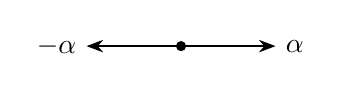
\begin{tikzpicture}[baseline=-3pt]
      \draw[root] (0,0) -- (1.2,0) node[right] {$\alpha$};
      \draw[root] (0,0) -- (-1.2,0) node[left] {$-\alpha$};
      \node[dot,inner sep=1.3pt] at (0,0) {};
    \end{tikzpicture}
    \]

    \begin{exercise}
    This is the only rank $1$ reduced root system.
    \end{exercise}
  \item Rank $2$: $V = \R^2$ with the usual inner product.
    \begin{alist}
      \item $A_1 \times A_1$ (or $A_1 + A_1$):
        \[
        \begin{tikzpicture}[baseline=-3pt]
          \draw[root] (0,0) -- (1.2,0) node[right] {$e_1$};
          \draw[root] (0,0) -- (-1.2,0);
          \draw[root] (0,0) -- (0,1.2) node[above] {$e_2$};
          \draw[root] (0,0) -- (0,-1.2);
        \end{tikzpicture}
        \]
        This is not irreducible. The Weyl group is $\Z/2 \times \Z/2$.
      \item $A_2$: $\alpha = \alpha\cv$, $\beta = \beta\cv$,
        $(\alpha, \beta) = -1$.
        \[
        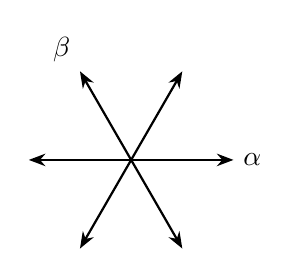
\begin{tikzpicture}[baseline=-3pt]
          \foreach \a in {0,60,...,300} \draw[root] (0,0) -- (\a:1.3);
          \node[right] at (0:1.3) {$\alpha$};
          \node[above left] at (120:1.3) {$\beta$};
        \end{tikzpicture}
        \]
        $W = S_3$ is the dihedral group of order $6$. This is the root system
        of $\sl_3$, as you should be able to establish (and we will shortly
        see).
      \item $B_2$: $\alpha = e_1$, $\beta = e_2 - e_1$; $(\alpha, \alpha) = 1$
        and $(\beta, \beta) = 2$. $\alpha$ and $\alpha + \beta$ are short
        roots; $\beta$ and $2\alpha + \beta$ are long roots.
        \[
        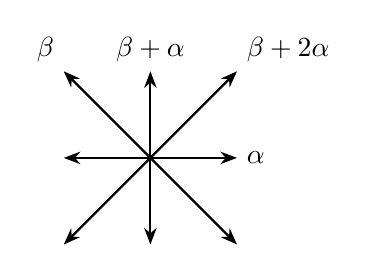
\begin{tikzpicture}[baseline=-3pt,scale=1.1]
          \foreach \a in {0,90,180,270} \draw[root] (0,0) -- (\a:1);
          \foreach \a in {45,135,225,315} \draw[root] (0,0) -- (\a:1.414);
          \node[right] at (0:1) {$\alpha$};
          \node[above left] at (135:1.414) {$\beta$};
          \node[above] at (90:1) {$\beta + \alpha$};
          \node[above right] at (45:1.414) {$\beta + 2\alpha$};
        \end{tikzpicture}
        \]
        $W$ is the dihedral group of order $8$. This is the root system of
        $\spl_4$ and $\so_5$.
      \item $G_2$: at this point, we clearly should look at all the dihedral
        groups, right? Unfortunately, no: the condition
        $(\alpha, \beta\cv) \in \Z$ rules out all but the dihedral group of
        order $12$. This is the root system of a Lie group, but not one of the
        classical ones (it is the automorphism group of the octonions).
        \[
        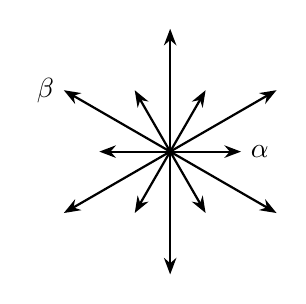
\begin{tikzpicture}[baseline=-3pt]
          \foreach \a in {0,60,...,300} \draw[root] (0,0) -- (\a:0.9);
          \foreach \a in {30,90,...,330} \draw[root] (0,0) -- (\a:1.56);
          \node[right] at (0:0.9) {$\alpha$};
          \node[left] at (150:1.56) {$\beta$};
        \end{tikzpicture}
        \]
        Here $\alpha$ is short, $\beta$ is long, $(\beta, \beta) = 3(\alpha, \alpha)$,
        and the angle between them is $150^\circ$.
    \end{alist}
\end{enumerate}
\end{example}

\begin{exercise}
All of these are indeed root systems. They are the only rank $2$ reduced root
systems, and $A_2$, $B_2$, and $G_2$ are irreducible.
\end{exercise}

\begin{lemma}
If $R$ is a root system, so is $R\cv = \setc{\alpha\cv}{\alpha \in R}$.
\end{lemma}

\begin{exercise}
Prove it.
\end{exercise}

\begin{definition}
$R$ is \emph{simply laced} if all the roots have the same length.
\end{definition}

\begin{exercise}
If $R$ is simply laced, then $(R, V) \cong (R', V')$ where $(\alpha, \alpha) = 2$
for all $\alpha \in R'$ (i.e.\ $\alpha = \alpha\cv$). [\emph{Hint:} If
irreducible, rescale; if not, break up into a direct sum of irreducibles.]
\end{exercise}

We would like to look at roots as coming from a lattice. We will see why
length $2$ is so useful.

\begin{definition}
A \emph{lattice} $L$ is a finitely generated free abelian group
($\cong \Z^l$ for some $l$) with a bilinear form $L \times L \to \Z$, such that
$(L \otimes_\Z \R, (\,,\,))$ is an inner product space. A \emph{root} of $L$ is
an $\alpha \in L$ such that $(\alpha, \alpha) = 2$. We write
$R_L = \setc{l \in L}{(l, l) = 2}$ for the roots of $L$.
\end{definition}

Note that $\alpha \in R_L \implies s_\alpha(L) \subseteq L$.

\begin{lemma}
$R_L$ is a simply laced root system in $\R R_L$.
\end{lemma}

\begin{proof}
The only non-obvious claim is $|R_L| < \infty$. However, $R_L$ is the
intersection of a compact set (the sphere of radius $\sqrt 2$) with a discrete
set (the lattice), so is finite.
\end{proof}

\begin{definition}
We say that $L$ is \emph{generated by roots} if $\Z R_L = L$. Note that then
$L$ is an \emph{even lattice}, i.e.\ $(l, l) \in 2\Z$ for all $l \in L$.
\end{definition}

\begin{example}
$L = \Z\alpha$ with $(\alpha, \alpha) = \lambda$. If $\lambda = 2$ then
$R_L = \{\pm\alpha\}$ and $L = \Z R_L$; if $\frac{k^2\lambda}{2} \neq 1$ for
all $k$ then $R_L = \emptyset$.
\end{example}

We now characterise the simply laced root systems.
\begin{enumerate}
  \item $A_n$. Consider $\Z^{n+1} = \bigoplus_{i=1}^{n+1} \Z e_i$ with
    $(e_i, e_j) = \delta_{ij}$ (the square lattice). Define
    \[
      L = \setc{l \in \Z^{n+1}}{(l, e_1 + \dots + e_{n+1}) = 0}
        = \Bigl\{\sum a_ie_i \Bigm| \sum a_i = 0\Bigr\} \cong \Z^n.
    \]
    Then $R_L = \setc{e_i - e_j}{i \neq j}$, $\#R_L = n(n + 1)$, and
    $\Z R_L = L$.

    If $\alpha = e_i - e_j$ then $s_\alpha$ applied to a vector with
    coordinates $x_1, \dots, x_{n+1}$ (in the basis $e_1, \dots, e_{n+1}$)
    swaps the $i$th and $j$th coordinates; therefore,
    $W = \langle s_{e_i - e_j}\rangle = S_{n+1}$.

    $(R_L, \R L)$ is the root system of type $A_n$. Note that $n$ is the rank
    of the root system, not the index of the associated Lie algebra.

    \begin{exercise}\leavevmode
    \begin{alist}
      \item ``You should not believe a word I say'': check these statements!
      \item Draw $L \subseteq \Z^{n+1}$ and $R_L$ for $n = 1, 2$. Check that
        $A_1$ and $A_2$ agree with the previous pictures.
      \item Show that the root system of $\sl_{n+1}$ has type $A_n$.
    \end{alist}
    \end{exercise}
  \item $D_n$. Consider the square lattice $\Z^n$. The roots are
    $R_{\Z^n} = \setc{\pm e_i \pm e_j}{i \neq j}$. Set
    \[
      L = \Z R_L = \Bigl\{ l = \sum a_ie_i \Bigm| a_i \in \Z,\ \sum a_i \text{ even} \Bigr\}.
    \]
    $s_{e_i - e_j}$ swaps the $i$th and $j$th coordinates as before;
    $s_{e_i + e_j}$ swaps them and flips the signs of both.

    $(R_L, \R R_L)$ is called $D_n$; $\#R_L = 2n(n - 1)$. The Weyl group is
    \[
      W = (\Z/2)^{n-1} \rtimes S_n,
    \]
    where $(\Z/2)^{n-1}$ is the normal subgroup of sign changes of an even
    number of coordinates.

    \begin{exercise}\leavevmode
    \begin{alist}
      \item Check these statements!
      \item $D_n$ is irreducible if $n \geq 3$.
      \item $R_{D_3} = R_{A_3}$, $R_{D_2} = R_{A_1} \times R_{A_1}$.
      \item The root system of $\so_{2n}$ has type $D_n$.
    \end{alist}
    \end{exercise}
\end{enumerate}

\lecture{12} We continue our classification of the simply laced root systems:
\begin{enumerate}
  \item $E_8$. Let
    \[
      \Gamma_n = \Bigl\{(k_1, \dots, k_n) \Bigm| \text{either all } k_i \in \Z
        \text{ or all } k_i \in \Z + \tfrac12, \text{ and } \sum k_i \in 2\Z\Bigr\}.
    \]
    Consider $\alpha = (\frac12, \frac12, \dots, \frac12) \in \Gamma_n$, and
    note that $(\alpha, \alpha) = n/4$. Thus, if $\Gamma_n$ is an even lattice,
    we must have $8 \mid n$.

    \begin{exercise}\leavevmode
    \begin{alist}
      \item $\Gamma_{8n}$ is a lattice.
      \item For $n > 1$ the roots of $\Gamma_{8n}$ form a root system of type
        $D_{8n}$.
      \item The roots in $\Gamma_8$ are
        $\setc{\pm e_i \pm e_j}{i \neq j} \cup
        \setc{\frac12(\pm e_1 \pm e_2 \pm \dots \pm e_8)}{\text{an even number of } - \text{ signs}}$.
    \end{alist}
    \end{exercise}

    The root system of $\Gamma_8$ is called the root system of type $E_8$.
    The number of roots is
    \[
      \#R_{\Gamma_8} = \binom{8}{2} \cdot 4 + 128 = 240.
    \]
    To check that you're awake: the dimension of the associated Lie algebra is
    $240 + \rank(R_{\Gamma_8}) = 248$.

    \begin{remark}
    $E_8$ is weird. Its smallest nontrivial representation is the adjoint
    representation, of dimension $248$. This is quite unlike $\so_n$, $\sl_n$,
    etc., which had dimension $O(n^2)$ and an $n$-dimensional representation.
    There isn't a good understanding of why $E_8$ is like that.
    \end{remark}

    \begin{exercise}
    Can you compute $\#W$, the order of the Weyl group of $E_8$?
    [\emph{Answer:} $2^{14} \cdot 3^5 \cdot 5^2 \cdot 7$.]
    \end{exercise}

    \begin{exercise}
    If $R$ is a root system and $\alpha \in R$, then $\alpha^\perp \cap R$ is a
    root system (in the space it spans).
    \end{exercise}
  \item $E_7$ and $E_6$. We will now apply this to $\Gamma_8$. Let
    $\alpha = \frac12(1, 1, \dots, 1)$ and $\beta = e_7 + e_8$.

    \begin{definition}
    $\alpha^\perp \cap R_{\Gamma_8}$ is a root system of type $E_7$.
    $\langle \alpha, \beta\rangle^\perp \cap R_{\Gamma_8}$ is a root system of
    type $E_6$.
    \end{definition}

    \begin{exercise}
    Show $\#R_{E_7} = 126$ and $\#R_{E_6} = 72$. Describe the corresponding
    root lattices.
    \end{exercise}

    \begin{remark}
    These lattices are reasonably natural objects. Indeed, if we took the
    associated algebraic group and its maximal torus, there is a natural
    lattice associated with it coming from the fundamental group.
    Equivalently, we can think of the group homomorphisms to (or from)
    $\C^\times$. This isn't quite the root lattice, but it's closely related
    (and we might say more about it later).
    \end{remark}
\end{enumerate}

\begin{theorem}\leavevmode
\begin{enumerate}
  \item (``ADE classification'') The complete list of irreducible simply laced
    root systems is
    \[
      A_n,\ n \geq 1, \qquad D_n,\ n \geq 4, \qquad E_6, \qquad E_7, \qquad E_8.
    \]
    No two root systems in this list are isomorphic.
  \item The remaining irreducible reduced root systems are denoted by
    \[
      B_2 = C_2, \qquad B_n,\ C_n,\ n \geq 3, \qquad F_4, \qquad G_2,
    \]
    where
    \begin{align*}
      R_{B_n} &= \setc{\pm e_i,\ \pm e_i \pm e_j}{i \neq j} \subseteq \Z^n,\\
      R_{C_n} &= \setc{\pm 2e_i,\ \pm e_i \pm e_j}{i \neq j} \subseteq \Z^n,
    \end{align*}
    with $R_{C_n}\cv = R_{B_n}$. The root system of type $B_n$ corresponds to
    $\so_{2n+1}$, and the root system of type $C_n$ corresponds to
    $\spl_{2n}$. The Weyl groups are
    \[
      W_{B_n} = W_{C_n} = (\Z/2)^n \rtimes S_n.
    \]
    The root system $F_4$ is defined as follows: let
    $Q = \setc{(k_1, \dots, k_4)}{\text{all } k_i \in \Z \text{ or all } k_i \in \Z + \frac12}$
    and take
    \[
      R_{F_4} = \setc{\alpha \in Q}{(\alpha, \alpha) = 2 \text{ or } (\alpha, \alpha) = 1}
        = \Bigl\{\pm e_i,\ \pm e_i \pm e_j\ (i \neq j),\
          \tfrac12(\pm e_1 \pm \dots \pm e_4)\Bigr\}.
    \]
\end{enumerate}
\end{theorem}

\begin{remark}
The duality between $R_{B_n}$ and $R_{C_n}$ suggests some form of duality
between $\so_{2n+1}$ and $\spl_{2n}$. We will see it later.
\end{remark}

To prove this theorem, we will first choose a good basis for $V$ (the space
spanned by the root lattice). Choose $f\colon V \to \R$ linear such that
$f(\alpha) \neq 0$ for all $\alpha \in R$.

\begin{definition}
A root $\alpha \in R$ is \emph{positive}, $\alpha \in R^+$, if $f(\alpha) > 0$.
A root $\alpha \in R$ is \emph{negative}, $\alpha \in R^-$, if $f(\alpha) < 0$.
(Equivalently, $-\alpha \in R^+$.) A root $\alpha \in R^+$ is \emph{simple},
$\alpha \in \Pi$, if $\alpha$ is not the sum of two positive roots.
\end{definition}

\begin{example}\leavevmode
\begin{enumerate}
  \item $A_n$: the roots are $R = \setc{e_i - e_j}{i \neq j}$. Choose
    \[
      f(e_1) = n + 1,\ f(e_2) = n,\ \dots,\ f(e_{n+1}) = 1.
    \]
    Then $R^+ = \setc{e_i - e_j}{i < j}$. Since $f(R) \subseteq \Z$, if
    $f(\alpha) = 1$ then $\alpha$ must be simple. Therefore,
    $\Pi \supseteq \{e_1 - e_2, \dots, e_n - e_{n+1}\}$. On the other hand, it
    is clear that the positive integer span of these is $R^+$, so in fact we
    have equality.
  \item $B_n$: $R = \setc{\pm e_i,\ \pm e_i \pm e_j}{i \neq j}$. Take
    $f(e_1) = n, \dots, f(e_n) = 1$. Then
    $R^+ = \setc{e_i,\ e_i \pm e_j}{i < j}$ and
    $\Pi = \{e_1 - e_2, \dots, e_{n-1} - e_n, e_n\}$.
  \item $C_n$: $R = \setc{\pm 2e_i,\ \pm e_i \pm e_j}{i \neq j}$.
    $R^+ = \setc{2e_i,\ e_i \pm e_j}{i < j}$ and
    $\Pi = \{e_1 - e_2, \dots, e_{n-1} - e_n, 2e_n\}$.
  \item $D_n$: $R = \setc{\pm e_i \pm e_j}{i \neq j}$,
    $\Pi = \{e_1 - e_2, \dots, e_{n-1} - e_n, e_{n-1} + e_n\}$.
  \item $E_8$: set $f(e_1) = 28 = 1 + 2 + \dots + 7$, and $f(e_i) = 9 - i$ for
    $i = 2, \dots, 8$. Then
    \[
      R^+ = \Bigl\{e_i \pm e_j\ (i < j),\ \tfrac12(e_1 \pm e_2 \pm \dots \pm e_8)
        \text{ with an even number of } - \text{ signs}\Bigr\}
    \]
    and
    \[
      \Pi = \Bigl\{\underbrace{e_2 - e_3, \dots, e_7 - e_8}_{f = 1},\
        \underbrace{\tfrac12(e_1 + e_8 - e_2 - \dots - e_7)}_{f = 1},\
        \underbrace{e_7 + e_8}_{f = 3}\Bigr\}.
    \]
\end{enumerate}
\end{example}

\begin{exercise}
Check all of these (by finding a suitable function $f$ where one is not
listed). Also find the simple roots for $E_6$, $E_7$, $F_4$, and $G_2$.
\end{exercise}

\begin{remark}
So far we have made two choices. We have chosen a maximal torus, and we have
chosen a function $f$. Neither of these matters. We may or may not prove this
about the maximal torus later; as for $f$, note that the space of functionals
$f$ is partitioned into cells within which we get the same notions of positive
roots. The Weyl group acts simply transitively on these cells, which should
show that the choice of $f$ does not affect the structure of the root system we
are deriving.
\end{remark}

\begin{proposition}\leavevmode
\begin{enumerate}
  \item $\alpha, \beta \in \Pi \implies \alpha - \beta \notin R$.
  \item $\alpha, \beta \in \Pi$, $\alpha \neq \beta \implies (\alpha, \beta\cv) \leq 0$
    (i.e.\ the angle between $\alpha$ and $\beta$ is at least $90^\circ$).
  \item Every $\alpha \in R^+$ can be written as $\alpha = \sum k_i\alpha_i$
    with $\alpha_i \in \Pi$ and $k_i \in \Z_{\geq 0}$.
  \item Simple roots are linearly independent.
  \item $\alpha \in R^+$, $\alpha \notin \Pi \implies$ there exists
    $\alpha_i \in \Pi$ such that $\alpha - \alpha_i \in R^+$.
  \item $R$ is irreducible iff $\Pi$ is indecomposable (i.e.\
    $\Pi \neq \Pi_1 \sqcup \Pi_2$ with $\Pi_1, \Pi_2$ nonempty and
    $(\Pi_1, \Pi_2) = 0$).
\end{enumerate}
\end{proposition}

\begin{exercise}
Prove this! (Either by a case-by-case analysis, which you should do in a few
cases anyway, or by finding a uniform proof from the axioms of a root system.)
\end{exercise}

We will now find another way to represent the root system. Let
$\Pi = \{\alpha_1, \dots, \alpha_l\}$, and let $a_{ij} = (\alpha_i\cv, \alpha_j)$.

\begin{definition}
$A = (a_{ij})$ is the \emph{Cartan matrix}.
\end{definition}

\begin{properties}\leavevmode
\begin{enumerate}
  \item $a_{ij} \in \Z$, $a_{ii} = 2$, $a_{ij} \leq 0$ for $i \neq j$.
  \item $a_{ij} = 0 \iff a_{ji} = 0$.
  \item $\det A > 0$.
  \item All principal minors of $A$ are positive.
\end{enumerate}
\end{properties}

\begin{proof}
The first two should be obvious from the above. To prove the third, note that
\[
  A = \begin{pmatrix}
        \frac{2}{(\alpha_1, \alpha_1)} & & 0\\
        & \ddots & \\
        0 & & \frac{2}{(\alpha_l, \alpha_l)}
      \end{pmatrix}
      \cdot \bigl((\alpha_i, \alpha_j)\bigr).
\]
The first matrix is diagonal with positive entries; the second one is the Gram
matrix of a positive definite bilinear form, and so has positive determinant.

The last property follows because any principal submatrix of $A$ (i.e.\ one
obtained by removing the same set of rows and columns) has the same form as
$A$.
\end{proof}

We will represent $A$ by a \emph{Dynkin diagram}. The vertices correspond to
simple roots. Between vertices $\alpha_i$ and $\alpha_j$ there are
$a_{ij}a_{ji}$ lines (note that this value can be $0$ or $1$ in the simply
laced diagrams, may be $2$ in $B_n$ or $C_n$, and may be $3$ in $G_2$). If
there are $2$ or $3$ lines, we put an arrow pointing towards the short root.
See figure~\ref{fig:dynkin}.

\begin{exercise}
Show the Dynkin diagrams are as we claim.
\end{exercise}

\begin{figure}[!htbp]
\centering
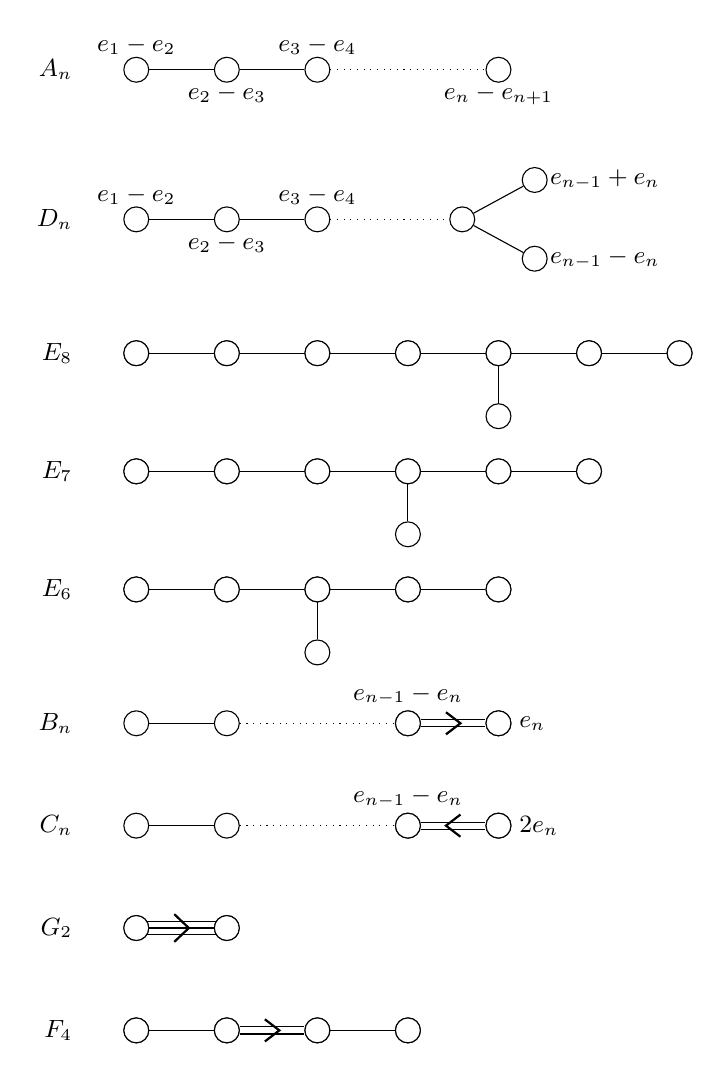
\begin{tikzpicture}[x=1.15cm,y=1cm,every node/.append style={font=\small}]
  % A_n
  \node[left] at (-0.6,0) {$A_n$};
  \node[node] (a1) at (0,0) {}; \node[node] (a2) at (1,0) {};
  \node[node] (a3) at (2,0) {}; \node[node] (a4) at (4,0) {};
  \draw (a1)--(a2)--(a3); \draw[dotted] (a3)--(a4);
  \node[above=2pt] at (a1) {$e_1 - e_2$}; \node[below=2pt] at (a2) {$e_2 - e_3$};
  \node[above=2pt] at (a3) {$e_3 - e_4$}; \node[below=2pt] at (a4) {$e_n - e_{n+1}$};
  % D_n
  \begin{scope}[yshift=-1.9cm]
  \node[left] at (-0.6,0) {$D_n$};
  \node[node] (d1) at (0,0) {}; \node[node] (d2) at (1,0) {};
  \node[node] (d3) at (2,0) {}; \node[node] (d4) at (3.6,0) {};
  \node[node] (d5) at (4.4,0.5) {}; \node[node] (d6) at (4.4,-0.5) {};
  \draw (d1)--(d2)--(d3); \draw[dotted] (d3)--(d4); \draw (d5)--(d4)--(d6);
  \node[above=2pt] at (d1) {$e_1 - e_2$}; \node[below=2pt] at (d2) {$e_2 - e_3$};
  \node[above=2pt] at (d3) {$e_3 - e_4$};
  \node[right=2pt] at (d5) {$e_{n-1} + e_n$}; \node[right=2pt] at (d6) {$e_{n-1} - e_n$};
  \end{scope}
  % E_8
  \begin{scope}[yshift=-3.6cm]
  \node[left] at (-0.6,0) {$E_8$};
  \foreach \i in {0,...,6} \node[node] (e\i) at (\i,0) {};
  \draw (e0)--(e6); \node[node] (eb) at (4,-0.8) {}; \draw (e4)--(eb);
  \foreach \i in {0,...,6} \node[node] at (\i,0) {};
  \end{scope}
  % E_7
  \begin{scope}[yshift=-5.1cm]
  \node[left] at (-0.6,0) {$E_7$};
  \foreach \i in {0,...,5} \node[node] (e\i) at (\i,0) {};
  \draw (e0)--(e5); \node[node] (eb) at (3,-0.8) {}; \draw (e3)--(eb);
  \foreach \i in {0,...,5} \node[node] at (\i,0) {};
  \end{scope}
  % E_6
  \begin{scope}[yshift=-6.6cm]
  \node[left] at (-0.6,0) {$E_6$};
  \foreach \i in {0,...,4} \node[node] (e\i) at (\i,0) {};
  \draw (e0)--(e4); \node[node] (eb) at (2,-0.8) {}; \draw (e2)--(eb);
  \foreach \i in {0,...,4} \node[node] at (\i,0) {};
  \end{scope}
  % B_n
  \begin{scope}[yshift=-8.3cm]
  \node[left] at (-0.6,0) {$B_n$};
  \node[node] (b1) at (0,0) {}; \node[node] (b2) at (1,0) {};
  \node[node] (b3) at (3,0) {}; \node[node] (b4) at (4,0) {};
  \draw (b1)--(b2); \draw[dotted] (b2)--(b3); \dbond{b3}{b4}
  \node[node] at (b3) {}; \node[node] at (b4) {};
  \node[above=3pt] at (b3) {$e_{n-1} - e_n$}; \node[right=4pt] at (b4) {$e_n$};
  \end{scope}
  % C_n
  \begin{scope}[yshift=-9.6cm]
  \node[left] at (-0.6,0) {$C_n$};
  \node[node] (c1) at (0,0) {}; \node[node] (c2) at (1,0) {};
  \node[node] (c3) at (3,0) {}; \node[node] (c4) at (4,0) {};
  \draw (c1)--(c2); \draw[dotted] (c2)--(c3); \dbond{c4}{c3}
  \node[node] at (c3) {}; \node[node] at (c4) {};
  \node[above=3pt] at (c3) {$e_{n-1} - e_n$}; \node[right=4pt] at (c4) {$2e_n$};
  \end{scope}
  % G_2
  \begin{scope}[yshift=-10.9cm]
  \node[left] at (-0.6,0) {$G_2$};
  \node[node] (g1) at (0,0) {}; \node[node] (g2) at (1,0) {};
  \tbond{g1}{g2} \node[node] at (g1) {}; \node[node] at (g2) {};
  \end{scope}
  % F_4
  \begin{scope}[yshift=-12.2cm]
  \node[left] at (-0.6,0) {$F_4$};
  \foreach \i in {0,...,3} \node[node] (f\i) at (\i,0) {};
  \draw (f0)--(f1); \dbond{f1}{f2} \draw (f2)--(f3);
  \foreach \i in {0,...,3} \node[node] at (\i,0) {};
  \end{scope}
\end{tikzpicture}
\caption{Dynkin diagrams (simply laced first). In $B_n$, $C_n$, $G_2$ and
$F_4$ the arrow points towards the short root.}
\label{fig:dynkin}
\end{figure}

\lecture{13}

\begin{exercise}
If $(R, V)$ is an irreducible root system with positive roots $R^+$, then there
is a \emph{unique} root $\theta \in R^+$ such that for all $\alpha \in \Pi$,
$\theta + \alpha \notin R^+$. This is called the \emph{highest root}.

At the moment, the easiest way to prove this is to examine all the root
systems we have. Later we'll give a uniform proof (and show the relationship
between $\theta$ and the adjoint representation).
\end{exercise}

\begin{example}
In $A_n$, the highest root is $e_1 - e_{n+1}$.
\end{example}

Define the ``extended Cartan matrix'' $\tilde A$ by setting
$\alpha_0 = -\theta$ (and then $\tilde A = (a_{ij})_{0 \leq i, j \leq l}$ with
$a_{ij} = (\alpha_i\cv, \alpha_j) = \frac{2(\alpha_i, \alpha_j)}{(\alpha_i, \alpha_i)}$).
The associated diagram is called the ``extended'' or ``affine'' Dynkin diagram.

\begin{example}
$A_1$ has $A = (2)$ and
$\tilde A = \bigl(\begin{smallmatrix} 2 & -2 \\ -2 & 2 \end{smallmatrix}\bigr)$.

$A_n$ has
\[
  A = \begin{pmatrix}
        2 & -1 & & \\
        -1 & 2 & \ddots & \\
        & \ddots & \ddots & -1\\
        & & -1 & 2
      \end{pmatrix}, \qquad
  \tilde A = \begin{pmatrix}
        2 & -1 & 0 & & -1\\
        -1 & 2 & -1 & & \\
        0 & -1 & 2 & \ddots & 0\\
        & & \ddots & \ddots & -1\\
        -1 & & 0 & -1 & 2
      \end{pmatrix}.
\]
\end{example}

Notice that $\tilde A$ satisfies almost the same conditions as the Cartan
matrix, i.e.
\begin{enumerate}
  \item $a_{ij} \in \Z$, $a_{ij} \leq 0$ for $i \neq j$, $a_{ii} = 2$;
  \item $a_{ij} = 0 \iff a_{ji} = 0$;
  \item $\det \tilde A = 0$, and every proper principal minor of $\tilde A$ is
    positive.
\end{enumerate}
The third property follows since $\tilde A$ is related to the Gram matrix for
$\alpha_0, \dots, \alpha_l$, which are not linearly independent.

\begin{exercise}
Write down $\tilde A$ and the extended Dynkin diagram for all types. To get you
started, in $B_n$ we have $\alpha_0 = -e_1 - e_2$, in $C_n$ we have
$\alpha_0 = -2e_1$, and in $D_n$ we have $\alpha_0 = -e_1 - e_2$.
\end{exercise}

\begin{exercise}
Show that $\tilde A_n^{(2)}$ (``twisted $A_n$'') also has determinant $0$. (See
figure~\ref{fig:affine}.)
\end{exercise}

\begin{exercise}
The Dynkin diagram of $A^T$ is the Dynkin diagram of $A$ with the arrows
reversed.
\end{exercise}

These diagrams (plus their transposes) are (almost) all the non-garbage Lie
algebras out there. (We'll be slightly more precise about the meaning of
``non-garbage'' later.)

\begin{theorem}
An irreducible (i.e., connected) Dynkin diagram is one of $A_n$, $B_n$, $C_n$,
$D_n$, $E_6$, $E_7$, $E_8$, $F_4$, and $G_2$.
\end{theorem}

\begin{proof}\leavevmode
\begin{enumerate}
  \item First, we classify the rank $2$ Dynkin diagrams, i.e.\ their Cartan
    matrices:
    \[
      A = \begin{pmatrix} 2 & -a \\ -b & 2 \end{pmatrix}
    \]
    with $\det A = 4 - ab > 0$. This leaves the options $(a, b) = (0, 0)$
    ($A_1 \times A_1$), $(1, 1)$ ($A_2$), $(2, 1)$ or $(1, 2)$ ($B_2$), and
    $(3, 1)$ or $(1, 3)$ ($G_2$).
  \item Observe that any subdiagram of a Dynkin diagram is a Dynkin diagram. In
    particular, since the affine Dynkin diagrams have determinant $0$, they
    are not subdiagrams of a Dynkin diagram.
  \item A Dynkin diagram contains no cycles. Indeed, let
    $\alpha_1, \dots, \alpha_n$ be distinct simple roots, and consider
    $\alpha = \sum \alpha_i/\sqrt{(\alpha_i, \alpha_i)}$. Then
    \[
      0 < (\alpha, \alpha) = n + \sum_{i<j}
        \frac{2(\alpha_i, \alpha_j)}{\sqrt{(\alpha_i, \alpha_i)(\alpha_j, \alpha_j)}}
        = n - \sum_{i<j} \sqrt{a_{ij}a_{ji}}.
    \]
    Therefore, $\sum_{i<j} \sqrt{a_{ij}a_{ji}} < n$. On the other hand, if we
    had a cycle on $n$ simple roots, it would have at least $n$ edges, giving
    $\sum_{i<j} \sqrt{a_{ij}a_{ji}} \geq n$, a contradiction.
  \item If a diagram is simply laced, it is $A$, $D$, or $E$.

    Suppose it's not of type $A$. Since $\tilde D_4$ is not a subdiagram, any
    branchings are at most $3$-way; and since $\tilde D_n$ is not a subdiagram
    for $n > 4$, there is exactly one branch point. Therefore, the diagram is
    T-shaped, with $p$, $q$, and $r$ vertices in each leg (counting the branch
    point in each). We call this shape $T_{p,q,r}$; e.g., $E_8 = T_{5,3,2}$.

    \begin{exercise}
    Finish the proof in one of two ways:
    \begin{alist}
      \item by using the fact that $\tilde E_6$, $\tilde E_7$, $\tilde E_8$ are
        not subdiagrams of a Dynkin diagram; or
      \item by showing $\det T_{p,q,r} = pq + pr + qr - pqr$, and concluding
        that $D_n$, $E_6$, $E_7$, and $E_8$ are the only possibilities. (E.g.:
        $\det E_8 = 15 + 10 + 6 - 30 = 1$.)
    \end{alist}
    \end{exercise}
  \item We now deal with the non-simply-laced diagrams.

    \begin{exercise}
    If there is a triple bond in the diagram, then the Dynkin diagram is
    $G_2$. (Note that we took care of one of the possibilities in
    $\tilde G_2$; you need to check the possibility of a double and a triple
    bond, and of two triple bonds.)
    \end{exercise}

    Finally, if there is a double bond in the diagram, then by $\tilde C_n$
    and $\tilde A_n^{(2)}$ there's only one of them, and by $\tilde B_n$ the
    diagram does not branch. If the double bond is in the middle, we have
    $F_4$ (since we don't have $\tilde F_4$); otherwise, we have $B_n$ or
    $C_n$. \qedhere
\end{enumerate}
\end{proof}

\begin{figure}[!htbp]
\centering
\begin{tikzpicture}[x=1.15cm,y=1cm,every node/.append style={font=\small}]
  % tilde A_n
  \node[left] at (-0.6,0) {$\tilde A_n$};
  \node[node] (a1) at (0,0) {}; \node[node] (a2) at (1,0) {};
  \node[node] (a3) at (2,0) {}; \node[node] (a4) at (4,0) {};
  \node[aff] (a0) at (2,1) {};
  \draw (a1)--(a2)--(a3); \draw[dotted] (a3)--(a4); \draw (a1)--(a0)--(a4);
  \foreach \v in {a1,a2,a3,a4} \node[node] at (\v) {}; \node[aff] at (a0) {};
  % tilde D_n
  \begin{scope}[yshift=-1.9cm]
  \node[left] at (-0.6,0) {$\tilde D_n$};
  \node[node] (d1) at (0,0.5) {}; \node[aff] (d0) at (0,-0.5) {};
  \node[node] (d2) at (0.8,0) {}; \node[node] (d3) at (1.8,0) {};
  \node[node] (d4) at (3.6,0) {};
  \node[node] (d5) at (4.4,0.5) {}; \node[node] (d6) at (4.4,-0.5) {};
  \draw (d1)--(d2)--(d0); \draw (d2)--(d3); \draw[dotted] (d3)--(d4);
  \draw (d5)--(d4)--(d6);
  \foreach \v in {d1,d2,d3,d4,d5,d6} \node[node] at (\v) {}; \node[aff] at (d0) {};
  \end{scope}
  % tilde E_8
  \begin{scope}[yshift=-3.6cm]
  \node[left] at (-0.6,0) {$\tilde E_8$};
  \foreach \i in {0,...,7} \node[node] (e\i) at (\i,0) {};
  \draw (e0)--(e7); \node[node] (eb) at (5,-0.8) {}; \draw (e5)--(eb);
  \foreach \i in {1,...,7} \node[node] at (\i,0) {}; \node[aff] at (e0) {};
  \end{scope}
  % tilde E_7
  \begin{scope}[yshift=-5.1cm]
  \node[left] at (-0.6,0) {$\tilde E_7$};
  \foreach \i in {0,...,6} \node[node] (e\i) at (\i,0) {};
  \draw (e0)--(e6); \node[node] (eb) at (3,-0.8) {}; \draw (e3)--(eb);
  \foreach \i in {0,...,5} \node[node] at (\i,0) {}; \node[aff] at (e6) {};
  \end{scope}
  % tilde E_6
  \begin{scope}[yshift=-6.6cm]
  \node[left] at (-0.6,0) {$\tilde E_6$};
  \foreach \i in {0,...,4} \node[node] (e\i) at (\i,0) {};
  \draw (e0)--(e4); \node[node] (eb) at (2,-0.8) {}; \node[aff] (ec) at (2,-1.6) {};
  \draw (e2)--(eb)--(ec);
  \foreach \i in {0,...,4} \node[node] at (\i,0) {}; \node[node] at (eb) {}; \node[aff] at (ec) {};
  \end{scope}
  % tilde B_n
  \begin{scope}[yshift=-9.1cm]
  \node[left] at (-0.6,0) {$\tilde B_n$};
  \node[node] (b1) at (0,0.5) {}; \node[aff] (b0) at (0,-0.5) {};
  \node[node] (b2) at (0.8,0) {}; \node[node] (b3) at (3,0) {};
  \node[node] (b4) at (4,0) {};
  \draw (b1)--(b2)--(b0); \draw[dotted] (b2)--(b3); \dbond{b3}{b4}
  \foreach \v in {b1,b2,b3,b4} \node[node] at (\v) {}; \node[aff] at (b0) {};
  \end{scope}
  % tilde C_n
  \begin{scope}[yshift=-10.5cm]
  \node[left] at (-0.6,0) {$\tilde C_n$};
  \node[aff] (c0) at (0,0) {}; \node[node] (c1) at (1,0) {};
  \node[node] (c2) at (2,0) {}; \node[node] (c3) at (4,0) {};
  \node[node] (c4) at (5,0) {};
  \dbond{c0}{c1} \draw (c1)--(c2); \draw[dotted] (c2)--(c3); \dbond{c4}{c3}
  \foreach \v in {c1,c2,c3,c4} \node[node] at (\v) {}; \node[aff] at (c0) {};
  \end{scope}
  % tilde G_2
  \begin{scope}[yshift=-11.8cm]
  \node[left] at (-0.6,0) {$\tilde G_2$};
  \node[aff] (g0) at (0,0) {}; \node[node] (g1) at (1,0) {};
  \node[node] (g2) at (2,0) {};
  \draw (g0)--(g1); \tbond{g1}{g2}
  \node[node] at (g1) {}; \node[node] at (g2) {}; \node[aff] at (g0) {};
  \end{scope}
  % tilde F_4
  \begin{scope}[yshift=-13.1cm]
  \node[left] at (-0.6,0) {$\tilde F_4$};
  \node[aff] (f0) at (0,0) {};
  \foreach \i in {1,...,4} \node[node] (f\i) at (\i,0) {};
  \draw (f0)--(f1)--(f2); \dbond{f2}{f3} \draw (f3)--(f4);
  \foreach \i in {1,...,4} \node[node] at (f\i) {}; \node[aff] at (f0) {};
  \end{scope}
  % tilde A_n^(2)
  \begin{scope}[yshift=-14.4cm]
  \node[left] at (-0.6,0) {$\tilde A_n^{(2)}$};
  \node[aff] (t0) at (0,0) {}; \node[node] (t1) at (1,0) {};
  \node[node] (t2) at (2,0) {}; \node[node] (t3) at (4,0) {};
  \node[node] (t4) at (5,0) {};
  \dbond{t0}{t1} \draw (t1)--(t2); \draw[dotted] (t2)--(t3); \dbond{t3}{t4}
  \foreach \v in {t1,t2,t3,t4} \node[node] at (\v) {}; \node[aff] at (t0) {};
  \end{scope}
\end{tikzpicture}
\caption{Affine Dynkin diagrams. The hatched vertex is the added root
$\alpha_0$.}
\label{fig:affine}
\end{figure}

\begin{exercise}
Compute the determinant of all the Cartan matrices.
\end{exercise}

\begin{example}
\[
  A_1\colon \det(2) = 2, \qquad
  A_2\colon \det \begin{pmatrix} 2 & -1 \\ -1 & 2 \end{pmatrix} = 3, \qquad
  A_3\colon \det = 4, \qquad \dots
\]
This comes out of the following: $SL_{n+1} = \setc{X}{\det X = 1}$ has centre
consisting of the $(n+1)$th roots of unity (i.e.\ a cyclic group of order
$n + 1$). Note that the order of the centre is equal to the determinant of the
Cartan matrix. This is true in general: the order of the centre of a simply
connected algebraic group with Lie algebra $\g$ and associated Cartan matrix
$A$ is equal to $\det A$.

In particular, this means that the simply connected algebraic group attached
to $E_8$ has no centre.
\end{example}

\section{Existence and uniqueness}

\lecture{14}

\subsection*{A. Independence of choices}

\begin{theorem}
All maximal tori are conjugate. (Recall that we are in the setting of
$\charac k = 0$, $k = \overline{k}$.) That is, if $\at$ and $\at'$ are two
maximal tori of $\g$, then there exists
\[
  g \in \Aut(\g)^0 = \setc{g \in GL(\g)}{g\colon \g \to \g \text{ is a Lie algebra homomorphism}}^0
\]
such that $g\at = \at'$. (Note: $\Aut(\g)$ is itself an algebraic group;
$\Aut(\g)^0$ is the connected component of $1$. Also, for semisimple $\g$,
$\Lie(\Aut \g) = \g$, since every derivation is inner.)
\end{theorem}

The proof is not very hard and involves a little bit of algebraic geometry; we
won't give it.

\begin{theorem}
All positive root systems $R^+$ are conjugate. That is, let $(V, R)$ be a root
system. Let $f_1, f_2\colon V \to \R$ satisfy $f_i(\alpha) \neq 0$ for all
$\alpha \in R$, and define $R^+_{(1)}$, $R^+_{(2)}$ accordingly. There exists a
unique $w \in W$ such that $wR^+_{(1)} = R^+_{(2)}$. (Consequently,
$w\Pi_1 = \Pi_2$ and we get the same Cartan matrix out of the two choices.)
\end{theorem}

The proof is quite easy, but we still won't give it.

\begin{corollary}
$\g$ determines the Cartan matrix, i.e.\ the Dynkin diagram, regardless of the
choices we made.
\end{corollary}

\subsection*{B. Uniqueness}

\begin{theorem}
For $i = 1, 2$, let $\g_i$ be semisimple Lie algebras with Cartan subalgebras
$\at_i$, root systems $R_i$, positive root systems $R_i^+$, simple roots
$\Pi_i$ and Cartan matrices $A_i$. Suppose that, after reordering indices,
$A_1 = A_2$. Then there exists an isomorphism of Lie algebras
$\phi\colon \g_1 \to \g_2$ such that $\phi(\at_1) = \at_2$,
$\phi(R_1) = R_2$, etc.
\end{theorem}

We will not prove this theorem, but we will say more about it.

\subsection*{C. Existence}

\begin{theorem}
Let $A$ be a Cartan matrix. There exists a semisimple Lie algebra whose Cartan
matrix is $A$.
\end{theorem}

\begin{remark}
We already know this for the infinite families, but a nice proof would not be
case-by-case.
\end{remark}

We will now talk about existence and uniqueness.

Let $\g$ be a semisimple Lie algebra, $\g = \at + \bigoplus_{\alpha \in R} \g_\alpha$,
and let the simple roots be $\Pi = \{\alpha_1, \dots, \alpha_l\}$. Choose
\[
  0 \neq E_i \in \g_{\alpha_i}, \quad F_i \in \g_{-\alpha_i}
  \text{ such that } (E_i, F_i)_{\ad} = \frac{2}{(\alpha_i, \alpha_i)}, \qquad
  H_i = \frac{2\nu^{-1}(\alpha_i)}{(\alpha_i, \alpha_i)}.
\]
Define $a_{ij} = (\alpha_i\cv, \alpha_j) = \frac{2(\alpha_i, \alpha_j)}{(\alpha_i, \alpha_i)}$.

We have the following commutation relations:
\begin{itemize}
  \item $[H_i, H_j] = 0$ (the torus commutes);
  \item $[H_i, E_j] = a_{ij}E_j$, since
    \[
      [H_i, E_j] = \alpha_j(H_i)E_j
        = \frac{\alpha_j\bigl(2\nu^{-1}(\alpha_i)\bigr)}{(\alpha_i, \alpha_i)}E_j
        = \frac{2(\alpha_i, \alpha_j)}{(\alpha_i, \alpha_i)}E_j;
    \]
  \item $[H_i, F_j] = -a_{ij}F_j$;
  \item $[E_i, F_j] = 0$ for $i \neq j$, since
    $[E_i, F_j] \in \g_{\alpha_i - \alpha_j}$ and $\alpha_i - \alpha_j \notin R$
    for $\alpha_i, \alpha_j \in \Pi$;
  \item $[E_i, F_i] = H_i$.
\end{itemize}

``Depending on your mood, these are either some of the relations or all of the
relations.'' We will see what this means.

Let $\fn^+ = \bigoplus_{\alpha \in R^+} \g_\alpha$,
$\fn^- = \bigoplus_{\alpha \in -R^+} \g_\alpha$. Then
$\g = \fn^+ + \at + \fn^-$. (Note that $\fn^+$ and $\fn^-$ are subalgebras, but
not ideals, of $\g$.)

\begin{lemma}
The $E_i$ generate $\fn^+$; the $F_i$ generate $\fn^-$; hence the $E_i, F_i$
generate $\g$ as a Lie algebra.
\end{lemma}

\begin{proof}
For a root $\alpha \in R^+$ write $\alpha = \sum k_i\alpha_i$ with
$k_i \in \Z_{\geq 0}$, and define the \emph{height} of $\alpha$ to be
$h(\alpha) = \sum k_i$. We now induct on the height of the root. Recall that if
$\alpha \in R^+$ and $\alpha$ is not simple, then there exists
$\alpha_i \in \Pi$ such that $\alpha - \alpha_i = \beta \in R^+$. By induction,
$\g_\beta$ is generated by the $E_i$. However, then
$\g_\alpha = [\g_\beta, \g_{\alpha_i}]$ is also generated by the $E_i$.

The corresponding claim about the $F_i$ follows immediately by taking $-R^+$ as
the positive roots.

Finally, $[E_i, F_i] = H_i$ and $\setc{H_i}{i = 1, \dots, l}$ is a basis for
$\at$ (recall the simple roots are a basis for $\at^*$).
\end{proof}

Let $A$ be a ``generalised Cartan matrix''. That is, $a_{ii} = 2$,
$a_{ij} = 0$ whenever $a_{ji} = 0$, and $a_{ij} \in \Z_{\leq 0}$ for
$i \neq j$ (but we do not include requirements of positive definiteness). Let
\begin{multline*}
  \gtil = \bigl\langle E_i, F_i, H_i \bigm| [H_i, H_j] = 0,\ [H_i, E_j] = a_{ij}E_j,\\
    [H_i, F_j] = -a_{ij}F_j,\ [E_i, F_j] = 0 \text{ for } i \neq j,\ [E_i, F_i] = H_i\bigr\rangle.
\end{multline*}
Clearly, if $A$ is the Cartan matrix of $\g$, then $\gtil \twoheadrightarrow \g$.
Are these all the relations? Not quite. Let
\[
  \gbar = \gtil\big/\bigl\langle (\ad E_i)^{1 - a_{ij}}E_j = 0,\
    (\ad F_i)^{1 - a_{ij}}F_j = 0 \text{ for } i \neq j\bigr\rangle
\]
(e.g., if $a_{ij} = 0$ then $E_i$ and $E_j$ commute, and if $a_{ij} = -1$ then
$[E_i, [E_i, E_j]] = 0$). These are called the ``Serre relations''.

\begin{remark}
They are called the Serre relations because they were discovered by
Harish-Chandra and Chevalley.
\end{remark}

\begin{exercise}
Check that the Serre relations hold in the classical Lie algebras.
\end{exercise}

\begin{theorem}\leavevmode
\begin{enumerate}
  \item If $A$ is indecomposable, then among the ideals of $\gtil$ meeting
    $\Span\{H_i\}$ trivially there is a unique maximal one, $\fr$. If $A$ is
    symmetrisable (for instance, if $A$ is a Cartan matrix), then $\gbar$ is
    the quotient $\gtil/\fr$, and if moreover $\det A \neq 0$ then $\gbar$ is
    simple. (But it need not be finite-dimensional!)
  \item Hence, if $\g$ is a finite-dimensional semisimple Lie algebra with
    Cartan matrix $A$, then the map $\gtil \to \g$ via $E_i \mapsto E_i$,
    $F_i \mapsto F_i$, $H_i \mapsto H_i$ (where on the left-hand side we have
    the canonical generators of $\gtil$ and on the right-hand side we have the
    elements of the root spaces we found above) factors through $\gbar$ and is
    surjective, so gives an isomorphism $\gbar \cong \g$.
\end{enumerate}
\end{theorem}

The second part of the theorem clearly implies the uniqueness. We also see that
existence is equivalent to the statement
\[
  \gbar \text{ is finite-dimensional} \iff A \text{ is a Cartan matrix}.
\]

\begin{definition}
$\gbar$ (for any $A$) is called a \emph{Kac--Moody algebra} (this time because
they were independently discovered by Kac and Moody).
\end{definition}

Most of the representation theory we will be talking about holds verbatim for
the Kac--Moody algebras. However, note that all we have given for them is a
finite presentation, which is not a very nice object. In particular, the root
spaces of these algebras need not be $1$-dimensional. The dimension of the root
space for any given root is computable but horrible, unless the matrix $A$ is
an affine Dynkin diagram. In that case, the Lie algebra is approximately
$\C c + \g \otimes \C[t, t^{-1}]$.

The Weyl group has a corresponding presentation:

\begin{theorem}[Presentation of the Weyl group]
Write $s_i = s_{\alpha_i}$; then
\[
  W = \bigl\langle s_1, \dots, s_l \bigm| s_i^2 = 1,\ (s_is_j)^{m_{ij}} = 1 \text{ for } i \neq j\bigr\rangle,
\]
where the $m_{ij}$ are defined in terms of the Cartan matrix as follows:
\[
  \begin{array}{c|cccc}
    a_{ij}a_{ji} & 0 & 1 & 2 & 3\\ \hline
    m_{ij} & 2 & 3 & 4 & 6
  \end{array}
\]
\end{theorem}

E.g., if $i$ and $j$ are not connected in the Dynkin diagram then
$s_is_j = s_js_i$, and if they are connected by a single edge, then
$s_is_js_i = s_js_is_j$. These are known as the ``braid relations''. In
$A_{n-1}$ they look like figure~\ref{fig:braid}.

\begin{figure}[!htbp]
\centering
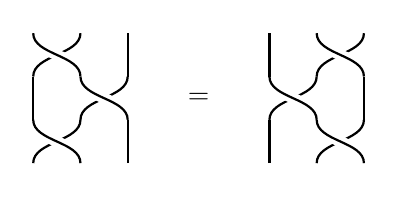
\begin{tikzpicture}[x=0.6cm,y=0.55cm,line width=0.8pt]
  % s_1 s_2 s_1 on strands 0,1,2; each crossing occupies one unit of height
  \newcommand{\cross}[2]{% #1 = left strand position, #2 = bottom height
    \draw (#1,#2) .. controls (#1,#2+0.5) and (#1+1,#2+0.5) .. (#1+1,#2+1);
    \draw[white,line width=4pt] (#1+1,#2) .. controls (#1+1,#2+0.5) and (#1,#2+0.5) .. (#1,#2+1);
    \draw (#1+1,#2) .. controls (#1+1,#2+0.5) and (#1,#2+0.5) .. (#1,#2+1);}
  \begin{scope}
    \cross{0}{0} \draw (2,0)--(2,1);
    \cross{1}{1} \draw (0,1)--(0,2);
    \cross{0}{2} \draw (2,2)--(2,3);
  \end{scope}
  \node at (3.5,1.5) {$=$};
  \begin{scope}[xshift=3cm]
    \cross{1}{0} \draw (0,0)--(0,1);
    \cross{0}{1} \draw (2,1)--(2,2);
    \cross{1}{2} \draw (0,2)--(0,3);
  \end{scope}
\end{tikzpicture}
\caption{Braid relation $s_1s_2s_1 = s_2s_1s_2$ in $A_{n-1}$, drawn on three
strands. We are asserting that the permutations are equal.}
\label{fig:braid}
\end{figure}

\lecture{15}

\begin{exercise}
Check, for each root system, that the relations claimed for the Weyl group do
hold. (This requires checking it for the rank $2$ root systems.) We will not
prove the isomorphism.
\end{exercise}

\begin{remark}
To show existence, we know that $\g = \at + \bigoplus_{\alpha \in R} \g_\alpha$,
so in principle existence should only require picking a basis $E_\alpha$ and
computing $[E_\alpha, E_\beta] = c_{\alpha\beta}E_{\alpha+\beta}$. How hard is
it to write down the $c_{\alpha\beta}$?

For a long time it was thought to be quite hard; however, with the discovery of
the affine Lie algebras, it turned out to be quite easy. We might even get to
doing it for the ADE algebras.
\end{remark}

\begin{remark}
So far the status of existence of a finite-dimensional simple Lie algebra
corresponding to an abstract root system is, for us, as follows: we have shown
that there exists a simple Lie algebra corresponding to each generalised
Cartan matrix, but not that it is finite-dimensional. Suppose that for the
$\gbar$ that we have defined we write
$\gbar = \at + \bigoplus_{\alpha \in R} \gbar_\alpha$ (where the torus comes
from the root system). We can ask two questions: (1) what is the relationship
between $R$ and the root system we started with? (2) What is
$\dim \gbar_\alpha$? While it is true that $W \cdot \Pi \subseteq R$, in
general there is not an equality between them. We call the roots in
$W \cdot \Pi$ ``real roots'', $R^{\mathrm{re}}$; for the real roots,
$\dim \gbar_\alpha = 1$. For finite-dimensional Lie algebras, all roots are
real. If $A$ is an affine Cartan matrix, then the semidefinite nature of it
means that there exists a root of length $0$, unique up to scaling, called the
imaginary root. The imaginary roots are pleasant and describable objects. For
a general, indefinite, Cartan matrix, there exists an algorithm for computing
$\dim \gbar_\alpha$, but the numbers are not very meaningful.
\end{remark}

\section{Representations}

Let $\g$ be a semisimple Lie algebra,
$\g = \at + \bigoplus_{\alpha \in R} \g_\alpha = \at + \fn^+ + \fn^-$. Let $V$
be a finite-dimensional representation of $\g$. (We don't quite need
finite-dimensional; we'll see exactly what we need a bit later.)

\begin{proposition}\leavevmode
\begin{enumerate}
  \item $V = \bigoplus_{\lambda \in \at^*} V_\lambda$, where
    $V_\lambda = \setc{v \in V}{t(v) = \lambda(t)v \ \forall t \in \at}$ (this
    is the weight space decomposition with respect to $\at$).
  \item If $V_\lambda \neq 0$, then $\lambda(h_\alpha) \in \Z$ for all
    $\alpha \in R$. (Here, $h_\alpha$ is the element of the $(\sl_2)_\alpha$,
    $h_\alpha = \nu^{-1}(\alpha\cv)$.)
\end{enumerate}
\end{proposition}

\begin{proof}
Since $V$ is a finite-dimensional representation of $\g$, it is a
finite-dimensional representation of $(\sl_2)_\alpha$. Therefore, $h_\alpha$
acts diagonalisably on $V$ with eigenvalues $\lambda(h_\alpha) \in \Z$. The
first assertion follows because the $h_\alpha$ commute and span $\at$.
\end{proof}

\begin{definition}
$Q = \Z R = \bigoplus_{\alpha_i \in \Pi} \Z\alpha_i$ is the \emph{lattice of
roots}.
$P = \setc{\gamma \in \Q R}{(\gamma, \alpha\cv) \in \Z \ \forall \alpha \in R}$
(the dual lattice) is the \emph{lattice of weights}. Note that the condition
can be checked by computing $(\gamma, \alpha_i\cv)$ for $\alpha_i \in \Pi$.
\end{definition}

Since $(\beta, \alpha\cv) \in \Z$ for $\beta, \alpha \in R$, we see that
$Q \subseteq P$. Also, if $V$ is a finite-dimensional representation of $\g$
and $V_\lambda \neq 0$, then $\lambda \in P$, as
$\lambda(h_\alpha) = (\lambda, \alpha\cv)$.

\begin{exercise}\leavevmode
\begin{enumerate}
  \item $|P/Q| < \infty$. In fact, $|P/Q| = \det A$, where $A$ is the Cartan
    matrix.
  \item $W(P) \subseteq P$, where $W$ is the Weyl group.
\end{enumerate}
\end{exercise}

\begin{example}
In $\sl_2$, $R = \{\pm\alpha\}$, $Q = \Z\alpha$, $(\alpha, \alpha) = 2$, so
$P = \Z\alpha/2$, and $|P/Q| = 2 = \det(2)$.
\end{example}

\begin{definition}
For $V$ a finite-dimensional representation of $\g$, define
\[
  \ch V = \sum_{\lambda \in P} \dim V_\lambda \cdot e^\lambda \in \Z[P].
\]
Here, $e^\lambda$ is a formal symbol ($e^\lambda e^\mu = e^{\lambda+\mu}$)
forming a basis for $\Z[P]$.
\end{definition}

``People are looking at me as if I'm speaking some language I don't speak, let
alone you don't speak.''

\begin{example}
For $\sl_2$, $P = \Z\alpha/2$. Write $z = e^{\alpha/2}$; then
$\ch L(n) = z^n + \dots + z^{-n} = \frac{z^{n+1} - z^{-(n+1)}}{z - z^{-1}}$.
\end{example}

\begin{example}
Let $\g = \sl_3$, and $V = \g$ the adjoint representation. Then
\[
  \ch V = 2 + z + w + zw + z^{-1} + w^{-1} + z^{-1}w^{-1},
\]
where $w = e^{\alpha_1}$, $z = e^{\alpha_2}$. See figure~\ref{fig:sl3-adjoint}.
\end{example}

\begin{figure}[!htbp]
\centering
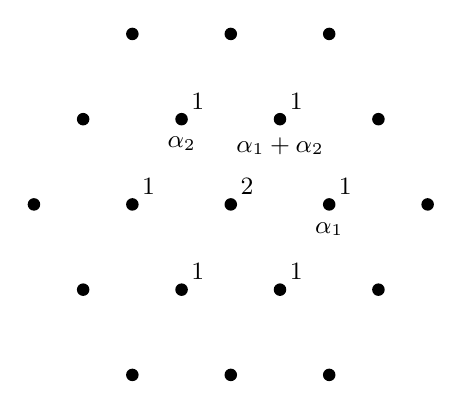
\begin{tikzpicture}[scale=1.25,every node/.append style={font=\small}]
  \foreach \i in {-2,...,2} \foreach \j in {-2,...,2} {
    \pgfmathsetmacro{\x}{\i + \j*cos(120)}
    \pgfmathsetmacro{\y}{\j*sin(120)}
    \pgfmathsetmacro{\r}{sqrt(\x*\x+\y*\y)}
    \ifdim \r pt < 2.1pt \node[dot] at (\x,\y) {}; \fi
  }
  \node[above right=0pt] at (0,0) {$2$};
  \foreach \a in {0,60,...,300} \node[above right=0pt] at (\a:1) {$1$};
  \node[below=3pt] at (0:1) {$\alpha_1$};
  \node[below=3pt] at (120:1) {$\alpha_2$};
  \node[below=3pt] at (60:1) {$\alpha_1 + \alpha_2$};
\end{tikzpicture}
\caption{Root lattice points of $\sl_3$ near the origin, with the dimensions
of the weight spaces of the adjoint representation. The six roots carry $1$,
the origin carries $2$, and the picture is $W$-invariant ($W = S_3$ here).}
\label{fig:sl3-adjoint}
\end{figure}

\begin{proposition}
If $V$ is a finite-dimensional representation of $\g$, then
$\dim V_\lambda = \dim V_{w\lambda}$ for all $w \in W$, i.e.\ $\ch V$ is
$W$-invariant, $\ch V \in \Z[P]^W$. (In particular, for $\sl_n$ this means that
the $\ch V$ are symmetric functions.)
\end{proposition}

We will sketch three proofs, of which the third one is the easiest, but the
first two reveal what is actually going on.

\begin{sketch}{1}
If $G$ is an algebraic group with Lie algebra $\g$ then (by a theorem)
$W = N(T)/T$ (where $T$ is the maximal torus in $G$ whose Lie algebra is
$\at$, and $N(T)$ is its normaliser).

\begin{example}
If $G = SL_n$ with $T$ the diagonal matrices, then $N(T)$ consists of the
matrices with exactly one nonzero entry in each row and column, and
$N(T)/T = S_n$, the permutation matrices.
\end{example}

That is, there exists $\dot w \in N(T)$ such that $\dot wT = w$. If $G$ acts on
$V$ (as it always does when $G$ is simply connected), then
$\dot w(V_\lambda) = V_{w\lambda}$, since
\[
  t\dot w(v) = \dot w(\dot w^{-1}t\dot w)v = \dot w\bigl(\lambda(\dot w^{-1}t\dot w)v\bigr).
\]
That is, $W$ is almost a subgroup of $G$. However, it is definitely not
actually a subgroup. E.g., in $SL_2$, we take
$\dot s = \bigl(\begin{smallmatrix} 0 & -1 \\ 1 & 0 \end{smallmatrix}\bigr)$,
and then
$\dot s^2 = \bigl(\begin{smallmatrix} -1 & 0 \\ 0 & -1 \end{smallmatrix}\bigr) \in T$
is not equal to $1$. That is, $W$ does not embed into $G$ and does not act on
$V$. (There is a small $2$-group, $\approx (\Z/2)^l$, that intervenes. This
$2$-group is also involved in determining the coefficients $c_{\alpha\beta}$.)
\end{sketch}

\begin{sketch}{2}
We can mimic the above argument in $\g$:
\[
  \begin{pmatrix} 0 & -1 \\ 1 & 0 \end{pmatrix}
  = \begin{pmatrix} 1 & 0 \\ 1 & 1 \end{pmatrix}
    \begin{pmatrix} 1 & -1 \\ 0 & 1 \end{pmatrix}
    \begin{pmatrix} 1 & 0 \\ 1 & 1 \end{pmatrix}
  = \exp(f)\exp(-e)\exp(f).
\]
Therefore, for each root $\alpha$ we define
$\dot s_\alpha = \exp(f_\alpha)\exp(-e_\alpha)\exp(f_\alpha)$, where the
matrix exponential is defined in the usual power series way.

\begin{exercise}\leavevmode
\begin{enumerate}
  \item If $V$ is a finite-dimensional representation of $\g$, then
    $e_\alpha$, $f_\alpha$ act nilpotently on $V$, so
    $\dot s_\alpha\colon V \to V$ is a well-defined finite sum.
  \item $\dot s_\alpha^2 = \epsilon_\alpha\colon V_\lambda \to V_\lambda$,
    where $\epsilon_\alpha^2 = 1$ and $\epsilon_\alpha$ acts by a constant.
    Determine this constant (in terms of $\lambda$).
  \item $\dot s_\alpha(V_\lambda) = V_{s_\alpha\lambda}$.
  \qedhere
\end{enumerate}
\end{exercise}
\end{sketch}

\begin{remark}
We did not really need $V$ to be finite-dimensional; what we need instead is
for each $e_\alpha$ and $f_\alpha$ to act \emph{locally nilpotently}. We say
$x\colon V \to V$ acts \emph{locally nilpotently} if for all $v \in V$ we have
$x^nv = 0$ for some $n$.
\end{remark}

\begin{exercise}
This is equivalent to saying that as an $(\sl_2)_\alpha$-module, $V$ splits
into a (possibly infinite) direct sum of finite-dimensional $\sl_2$-modules.
\end{exercise}

\begin{definition}
Such a $V$ is called \emph{integrable} (because you can ``integrate'' the Lie
algebra action to a group action).
\end{definition}

In the rest of the course, you can replace all instances of
``finite-dimensional'' by ``integrable'', and then all theorems and proofs will
work for the Kac--Moody algebras as well.

\begin{sketch}{3}
If we're just working with $\sl_2$ anyway, we shouldn't need all the other
stuff.

\begin{exercise}
Consider $V$ as a representation of $(\sl_2)_\alpha \times \at$. Then $V$
splits up into a direct sum of strings, each of which is of the form
\[
  \lambda \qquad \lambda - \alpha \qquad \lambda - 2\alpha \qquad \cdots \qquad \lambda - m\alpha,
\]
where $m = \lambda(h_\alpha)$ for the top weight $\lambda$ of the string.
\end{exercise}

Such a string is obviously $s_\alpha$-invariant, since $s_\alpha$ will just
flip the string from left to right (as the reflection did in $\sl_2$).
\end{sketch}

\lecture{16}

\begin{definition}
For $\lambda, \mu \in \at^*$ write $\mu \leq \lambda$ to mean
$\lambda - \mu = \sum k_i\alpha_i$ with $k_i \in \N$. The points
$\setc{\mu \in P}{\mu \leq \lambda}$ are the lattice points in an obtuse cone
(figure~\ref{fig:cone}).
\end{definition}

\begin{figure}[!htbp]
\centering
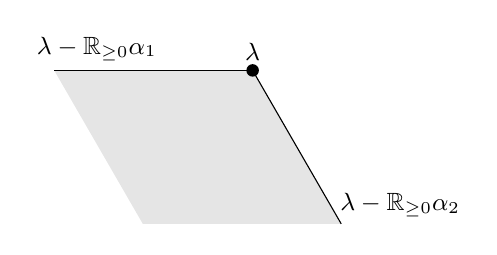
\begin{tikzpicture}[scale=0.9,every node/.append style={font=\small}]
  \fill[gray!20] (0,0) -- (180:2.8) -- ($(180:2.8)+(-60:2.5)$) -- (-60:2.5) -- cycle;
  \draw (0,0) -- (180:2.8);
  \draw (0,0) -- (-60:2.5);
  \node[dot] at (0,0) {};
  \node[above] at (0,0) {$\lambda$};
  \node[above] at (180:2.2) {$\lambda - \R_{\geq 0}\alpha_1$};
  \node[right] at (-60:2.2) {$\lambda - \R_{\geq 0}\alpha_2$};
\end{tikzpicture}
\caption{The cone $\setc{\mu}{\mu \leq \lambda}$ for $\sl_3$, bounded by the
directions $-\alpha_1$ and $-\alpha_2$.}
\label{fig:cone}
\end{figure}

\begin{definition}
If $V$ is a representation of $\g$, we say that $\mu \in P$ is a \emph{highest
weight} if $V_\mu \neq 0$ and $V_\lambda \neq 0 \implies \lambda \leq \mu$.

We say $v \in V_\gamma$ is a \emph{singular vector} if $v \neq 0$ and
$e_\alpha v = 0$ for all $\alpha \in R^+$. (Note that
$e_\alpha v \in V_{\gamma+\alpha}$, so if $\gamma$ is a highest weight, then
all nonzero elements of $V_\gamma$ are singular vectors.)

We say that $\mu$ is an \emph{extremal weight} if $w\mu$ is a highest weight
for some $w \in W$.
\end{definition}

\begin{example}
In the adjoint representation of $\sl_3$, the highest weight is
$\alpha_1 + \alpha_2$, and the six roots on the outer hexagon are the extremal
weights.
\end{example}

\begin{theorem}
Let $\g$ be a semisimple Lie algebra over $\C$.
\begin{enumerate}
  \item ``Complete reducibility'': if $V$ is a finite-dimensional
    representation of $\g$, then $V$ is a direct sum of irreducible
    representations of $\g$.

    Set $P^+ = \setc{\lambda \in P}{(\lambda, \alpha\cv) \geq 0 \ \forall \alpha \in R^+}$
    (of course, it's enough to check this on $\alpha \in \Pi$). This is the
    cone of \emph{dominant weights}. The assertion of the next parts of the
    theorem is that $P^+$ parametrises the finite-dimensional irreducible
    representations of $\g$, with $\lambda \mapsto L(\lambda)$. More
    precisely,
  \item Let $V$ be a finite-dimensional irreducible representation of $\g$,
    and $v \in V_\lambda$ a singular vector. Then
    \begin{alist}
      \item $\dim V_\lambda = 1$;
      \item $V_\mu \neq 0 \implies \mu \leq \lambda$, so $\lambda$ is a
        highest weight (and $v$ a highest-weight vector);
      \item $\lambda(h_i) \in \N$ for all $i$, i.e.\ $\lambda \in P^+$.
    \end{alist}
    Moreover, if $W$ is another finite-dimensional irreducible representation
    of $\g$ with highest weight $\lambda$, and $w \in W_\lambda$, $w \neq 0$,
    then there exists a unique isomorphism $V \to W$ mapping $v \mapsto w$.
    (Of course, given they are irreducible representations, if there is an
    isomorphism, there is a one-dimensional family of them, so we would pin
    down the exact one by sending $v \mapsto w$. That is, uniqueness is not
    the nontrivial statement here.)
  \item Given $\lambda \in P^+$, there exists a finite-dimensional irreducible
    representation with highest weight $\lambda$, called $L(\lambda)$.
  \item There is a formula for $\ch L(\lambda)$ (the Weyl character formula),
    to be stated later.
\end{enumerate}
\end{theorem}

\begin{remark}
For Kac--Moody algebras, we need a slight modification, since it is no longer
obvious that we will have highest-weight vectors. We need to work in the
category of integrable highest-weight representations instead.
\end{remark}

\begin{corollary}
\[
  \ch L(\lambda) = e^\lambda + \sum_{\mu < \lambda} a_{\mu\lambda}e^\mu \in \Z[P],
\]
hence $\setc{\ch L(\lambda)}{\lambda \in P^+}$ are linearly independent (they
have different leading terms). On the other hand,
\[
  \ch L(\lambda) = m_\lambda + \sum_{\substack{\mu < \lambda\\ \mu \in P^+}} \tilde a_{\mu\lambda}m_\mu
    \in \Z[P]^W, \qquad \text{where } m_\mu = \sum_{\gamma \in W\mu} e^\gamma.
\]
Since the $\{m_\mu\}_{\mu \in P^+}$ clearly form a basis for $\Z[P]^W$, the
$\ch L(\lambda)$ form a basis of $\Z[P]^W$.
\end{corollary}

\begin{corollary}
If $V$ and $W$ are finite-dimensional representations of $\g$, then
$V \cong W \iff \ch V = \ch W$.
\end{corollary}

\begin{proof}
Complete reducibility, plus the fact that the characters of irreducibles form a
basis.
\end{proof}

\begin{definition}
Define $\omega_i \in P$ to be the dual basis to the simple (co)roots,
$(\omega_i, \alpha_j\cv) = \delta_{ij}$ for $i, j = 1, \dots, l$. These are
called the \emph{fundamental weights}.
\end{definition}

Then $P^+ = \bigoplus \Z_{\geq 0}\omega_i = \setc{\sum n_i\omega_i}{n_i \geq 0}$.
This is a fundamental domain for the action of $W$ on $P$. Each irreducible
representation will have a unique highest weight lying in this cone, which is
what parametrises the representation.

\begin{exercise}
Compute the $\omega_i$ for the simple Lie algebras $\sl_n$, $\so_{2n}$,
$\so_{2n+1}$, $\spl_{2n}$, etc., and draw the picture for $A_2$, $B_2$, and
$G_2$.
\end{exercise}

\begin{figure}[!htbp]
\centering
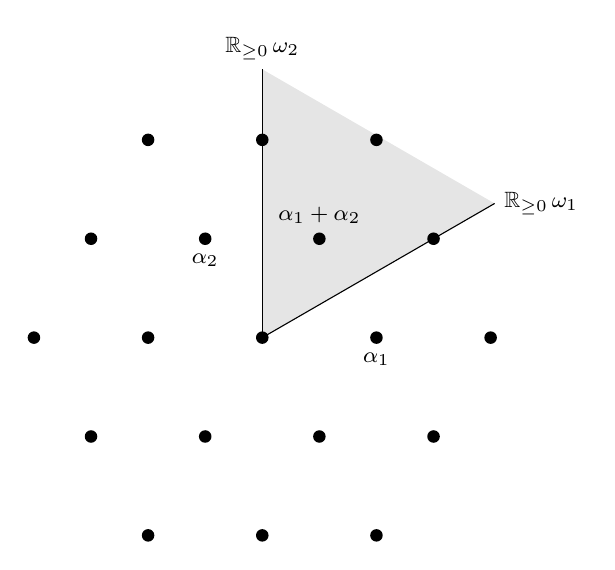
\begin{tikzpicture}[scale=1.45,every node/.append style={font=\footnotesize}]
  \fill[gray!20] (0,0) -- (90:2.35) -- (30:2.35) -- cycle;
  \draw (0,0) -- (90:2.35); \draw (0,0) -- (30:2.35);
  \foreach \i in {-2,...,2} \foreach \j in {-2,...,2} {
    \pgfmathsetmacro{\x}{\i + \j*cos(120)}
    \pgfmathsetmacro{\y}{\j*sin(120)}
    \pgfmathsetmacro{\r}{sqrt(\x*\x+\y*\y)}
    \ifdim \r pt < 2.1pt \node[dot] at (\x,\y) {}; \fi
  }
  \node[below=2pt] at (0:1) {$\alpha_1$};
  \node[below=2pt] at (120:1) {$\alpha_2$};
  \node[above=2pt] at (60:1) {$\alpha_1 + \alpha_2$};
  \node[above] at (90:2.35) {$\R_{\geq 0}\,\omega_2$};
  \node[right] at (30:2.35) {$\R_{\geq 0}\,\omega_1$};
\end{tikzpicture}
\caption{Cone of dominant weights for $\sl_3$, spanned by the fundamental
weights. The adjoint representation's highest weight is $\alpha_1 + \alpha_2$.}
\label{fig:dominant-sl3}
\end{figure}

\begin{exercise}
$\lambda \in P \implies \lambda = \sum \lambda(h_i)\omega_i$, where
$h_i = \nu^{-1}(\alpha_i\cv)$.
\end{exercise}

\begin{example}
For any $\g$, the trivial representation is $L(0)$.
\end{example}

For any simple $\g$, the adjoint representation $V = \g$ is irreducible. The
decomposition $\g = \at + \bigoplus_{\alpha \in R} \g_\alpha$ means that a
highest weight $\lambda$ is a root such that $\lambda + \alpha_i \notin R$ for
all $i$, i.e.\ $\lambda = \theta$, the highest root in $R^+$ (see
figure~\ref{fig:dominant-sl3}). (Therefore, the theorem of the highest weight
implies that $\theta$ is unique, as promised.)

\begin{example}
In $A_{n-1}$ ($n \geq 3$), the highest root is $\theta = e_1 - e_n$ (recall
$\alpha_i = e_i - e_{i+1}$ and $h_i$ is a diagonal matrix with $+1$ in the
$i$th position, $-1$ in the $(i+1)$th position, and $0$ elsewhere). We have
$\theta(h_1) = 1$, $\theta(h_2) = 0, \dots, \theta(h_{n-2}) = 0$,
$\theta(h_{n-1}) = 1$. We can label the Dynkin diagram by the $\theta(h_i)$:
\[
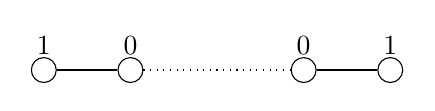
\begin{tikzpicture}[baseline=-3pt,x=1.1cm]
  \node[node] (p1) at (0,0) {}; \node[node] (p2) at (1,0) {};
  \node[node] (p3) at (3,0) {}; \node[node] (p4) at (4,0) {};
  \draw (p1)--(p2); \draw[dotted] (p2)--(p3); \draw (p3)--(p4);
  \node[above=2pt] at (p1) {$1$}; \node[above=2pt] at (p2) {$0$};
  \node[above=2pt] at (p3) {$0$}; \node[above=2pt] at (p4) {$1$};
\end{tikzpicture}
\]
The labels give the decomposition $\theta = \omega_1 + \omega_{n-1}$ of
$\theta$ into fundamental weights.
\end{example}

\begin{exercise}
Compute the $\theta(h_i)$ for all the simple Lie algebras.
\end{exercise}

\begin{example}
Other representations of $\sl_n$: we have the standard representation,
$\C^n$, with weight basis $v_1, \dots, v_n$ and weights $e_1, \dots, e_n$
(recall $\sum e_i = 0$). The highest weight is $e_1$ (as
$e_1 > e_2 > \dots > e_n$, since $e_1 - e_2, e_2 - e_3, \dots \in R^+$).
Therefore, $\C^n = L(\omega_1)$, and
\[
  \ch \C^n = e^{e_1} + \dots + e^{e_n} = z_1 + \dots + z_n,
\]
where $z_i = e^{e_i} \in \Z[P] = \Z[z_1^{\pm 1}, \dots, z_n^{\pm 1}]/(z_1\cdots z_n = 1)$.
\end{example}

Now, if $V$ and $W$ are representations of $\g$, then so is $V \otimes W$ (via
$x \in \g$ acting by $x \otimes 1 + 1 \otimes x$). In particular,
$V \otimes V$ is a representation. Note that
$\sigma\colon V \otimes V \to V \otimes V$, $a \otimes b \mapsto b \otimes a$,
commutes with the $\g$-action, so the eigenspaces of $\sigma$ are
$\g$-modules. That is, $S^2V$ and $\Lambda^2V$ are $\g$-modules. In general,
these need not be irreducible, but they are for $V = \C^n$ and $\g = \sl_n$, as
we check below.

Consider $\Lambda^s\C^n$ (for $s \leq n - 1$). This has weight basis
$v_{i_1} \wedge \dots \wedge v_{i_s}$ for $i_1 < \dots < i_s$, and the weight
of this is $e_{i_1} + \dots + e_{i_s}$, as is clear from the action. Therefore,
\[
  E_i(v_{i_1} \wedge \dots \wedge v_{i_s}) = 0 \text{ for all } i
  \iff v_{i_1} \wedge \dots \wedge v_{i_s} = v_1 \wedge \dots \wedge v_s,
\]
i.e.\ this is the only singular vector (up to scalars). Note that its weight
is $\omega = e_1 + \dots + e_s$, which is the $s$th fundamental weight, as
$(\omega, e_i - e_{i+1}) = \delta_{is}$. Therefore,
\[
  \Lambda^s\C^n = L(\omega_s) \text{ is a \emph{fundamental representation}.}
\]
In particular, $\Lambda^{n-1}\C^n \cong (\C^n)^* = L(\omega_{n-1})$.

Consider $S^m\C^n$. It has weight basis $v_{i_1}\cdots v_{i_m}$ with
$i_1 \leq \dots \leq i_m$ and weight $e_{i_1} + \dots + e_{i_m}$. We have
\[
  E_i(v_{i_1}\cdots v_{i_m}) = 0 \text{ for all } i
  \iff v_{i_1}\cdots v_{i_m} = v_1\cdots v_1 = v_1^m,
\]
i.e.\ $S^m\C^n$ is an irreducible representation isomorphic to
$L(m\omega_1)$.

\begin{exercise}
Check that the above is true. Compute $\ch \Lambda^s\C^n$ and
$\ch S^m\C^n$. Find a closed formula for the generating functions
\[
  \sum_{m \geq 0} (\ch S^m\C^n)q^m, \qquad \sum_{m \geq 0} (\ch \Lambda^m\C^n)q^m.
\]
\end{exercise}

\lecture{17}

\begin{exercise}\leavevmode
\begin{enumerate}
  \item If $V$ and $W$ are $\g$-modules, $V$ finite-dimensional, then
    $V^* \otimes W \cong \Hom(V, W)$ as $\g$-modules, via
    $v^* \otimes w \mapsto (v \mapsto v^*(v) \cdot w)$.

    \begin{remark}
    If $V$ is a $\g$-module, $V^*$ is a $\g$-module with action
    $(x \cdot \lambda)(v) = -\lambda(xv)$. The $-$ sign comes from
    differentiating the group action, $(g \cdot \lambda)(v) = \lambda(g^{-1}v)$.
    \end{remark}
  \item Show that if $V = \C^n$ and $\g = \sl_n$, then
    $V \otimes V^* \cong \sl_n \oplus \C$, adjoint plus trivial
    representations (where the trivial representation comes from
    $\Id \in \Hom_\g(V, V)$). In contrast, $V \otimes V \cong S^2V \oplus \Lambda^2V$
    always.
\end{enumerate}
\end{exercise}

\begin{exercise}
Let $\g = \so_n$ with $n = 3$ or $n \geq 5$, or $\g = \spl_{2l}$ with $2l = n$
and $l \geq 2$, and let $V = \C^n$.
\begin{enumerate}
  \item Compute the highest weight of this representation.
  \item $V \cong V^*$ via the form defining $\g$, so $V \otimes V$ has at least
    three components (since it must contain the trivial representation). Show
    that it has exactly three, describe them, and find the highest weights.
\end{enumerate}
\end{exercise}

We will now devote ourselves to proving Theorem~8.3, classifying all the
representations of semisimple Lie algebras.

Let $\g$ be any Lie algebra with a non-degenerate invariant bilinear form
$(\,,\,)$, e.g., $\g$ semisimple and $(\,,\,) = (\,,\,)_{\ad}$. Let
$x_1, \dots, x_N$ be a basis of $\g$, and $x^1, \dots, x^N$ the dual basis (so
$(x_i, x^j) = \delta_{ij}$).

\begin{definition}
$\Omega = \sum x_ix^i$ is the \emph{Casimir} of $\g$.
\end{definition}

\begin{remark}
For the moment, $\Omega$ is an operator on any representation of $\g$.
However, we will in a moment define the ``universal enveloping algebra of
$\g$'', and that is where $\Omega$ naturally lives.
\end{remark}

\begin{lemma}
For all $x \in \g$, we have $[\Omega, x] = 0$.
\end{lemma}

\begin{proof}[Proof 1, coordinate-based]
$[\Omega, x] = [\sum x_ix^i, x]$. Since $\ad x$ is a derivation, we rewrite
this as $\sum x_i[x^i, x] + \sum [x_i, x]x^i$. Write
$[x^i, x] = \sum_j a_{ij}x^j$ and $[x_i, x] = \sum_j b_{ij}x_j$. Then
\begin{align*}
  a_{ij} &= ([x^i, x], x_j) = ([x_j, x^i], x),\\
  b_{ij} &= ([x_i, x], x^j) = ([x^j, x_i], x) = -a_{ji}.
\end{align*}
Thus,
\[
  [\Omega, x] = \sum_{i,j} a_{ij}x_ix^j + \sum_{i,j} b_{ij}x_jx^i = 0. \qedhere
\]
\end{proof}

\begin{proof}[Proof 2, without coordinates]
We have maps of $\g$-modules
$\C \hookrightarrow \End(\g) \cong \g \otimes \g^* \cong \g \otimes \g$ (the
first map is via $\lambda \mapsto \lambda\Id$, i.e.\
$1 \mapsto \sum x_i \otimes x^i$; the last isomorphism is via the bilinear
form). Since $\g$ acts on $V$, we have a map of $\g$-modules
$\g \to \End(V)$. Finally, we have a map of $\g$-modules
$\End(V) \otimes \End(V) \to \End(V)$ by multiplication. This finally gives
\[
  \C \hookrightarrow \g \otimes \g^* \cong \g \otimes \g \to \End(V) \otimes \End(V) \to \End(V)
\]
sending $1 \mapsto \Omega$. Therefore, $\Omega$ generates a trivial
$\g$-submodule of $\End(V)$, which is equivalent to saying $[\Omega, x] = 0$
for all $x \in \g$.
\end{proof}

Now let $\g$ be semisimple, $\g = \at \oplus \bigoplus_{\alpha \in R} \g_\alpha$,
and $(\,,\,)_{\ad}$ the Killing form. Choose a basis $u_1, \dots, u_l$ of
$\at$, $x_\alpha$ of $\g_\alpha$; choose the dual basis $u^1, \dots, u^l$ of
$\at$ and $x^{-\alpha}$ of $\g_{-\alpha}$ (so that $(x_\alpha, x^{-\alpha}) = 1$).
Normalise $x_\alpha$ so that $(x_\alpha, x_{-\alpha})_{\ad} = 1$, so that
$x^{-\alpha} = x_{-\alpha}$. Then $[x_\alpha, x_{-\alpha}] = \nu^{-1}(\alpha)$
by the structure theorem. Now,
\[
  \Omega = \sum u_iu^i + \sum_{\alpha \in R^+} (x_\alpha x_{-\alpha} + x_{-\alpha}x_\alpha)
         = \sum u_iu^i + 2\sum_{\alpha \in R^+} x_{-\alpha}x_\alpha + \sum_{\alpha \in R^+} \nu^{-1}(\alpha).
\]

\begin{definition}
$\rho = \frac12 \sum_{\alpha \in R^+} \alpha$.
\end{definition}

\begin{remark}
Of course, there will be an exercise to compute $\rho$ for all the simple Lie
algebras. However, we will state this exercise later, when it's more obvious
what $\rho$ is.
\end{remark}

\begin{remark}
If you like algebraic geometry, this is the square root of the anticanonical
bundle on the flag variety.
\end{remark}

Then
\[
  \Omega = \sum u_iu^i + 2\nu^{-1}(\rho) + 2\sum_{\alpha \in R^+} x_{-\alpha}x_\alpha.
\]

\begin{lemma}
Let $V$ be a $\g$-module, $v \in V$ a singular vector with weight $\lambda$
(i.e.\ $\fn^+v = 0$ and $tv = \lambda(t)v$). Then
$\Omega v = \bigl(|\lambda + \rho|^2 - |\rho|^2\bigr)v$.
\end{lemma}

\begin{proof}
Apply the most recent version of $\Omega$:
\[
  \Omega v = \Bigl(\sum \lambda(u_i)\lambda(u^i) + \lambda\bigl(2\nu^{-1}(\rho)\bigr)\Bigr)v
    + 2\sum_{\alpha \in R^+} x_{-\alpha}x_\alpha v
  = \bigl((\lambda, \lambda) + 2(\lambda, \rho)\bigr)v. \qedhere
\]
\end{proof}

In particular, if $V$ is irreducible and has a singular vector of weight
$\lambda$, then $\Omega$ acts on $V$ by $(\lambda, \lambda) + 2(\lambda, \rho)$,
by Schur's lemma.

\section{PBW theorem}

Let $\g$ be any Lie algebra over a field $k$.

\begin{definition}
The \emph{universal enveloping algebra} $\U\g$ of $\g$ is the associative
algebra over $k$ generated by $\g$ with relations $xy - yx = [x, y]$ for all
$x, y \in \g$.
\end{definition}

More formally, if $V$ is a vector space over $k$, then
\[
  TV = k + V + V \otimes V + V^{\otimes 3} + \dots = \bigoplus_{n \geq 0} V^{\otimes n}
\]
is the \emph{tensor algebra of $V$}, and is the free associative algebra
generated by $V$. Let $J$ be the two-sided ideal in $T\g$ generated by
$x \otimes y - y \otimes x - [x, y]$ for all $x, y \in \g$; then
$\U\g = T\g/J$.

\begin{exercise}
An \emph{enveloping algebra} for $\g$ is a linear map $i\colon \g \to A$, where
$A$ is an associative algebra, and $i(x)i(y) - i(y)i(x) = i([x, y])$. (For
example, if $V$ is a representation of $\g$, we can take $A = \End(V)$ and $i$
the action map.) Show that $\U\g$ is initial in the category of enveloping
algebras, i.e.\ any such map $i$ factors uniquely through $\U\g$.
\end{exercise}

\begin{remark}
This is old terminology: anywhere other than the above exercise and old
textbooks, ``enveloping algebra'' almost certainly means ``universal
enveloping algebra''.
\end{remark}

The Casimir operator naturally lives in $\U\g$; in fact, as we've shown, in
the centre $Z(\U\g)$.

Observe that $T\g$ is a graded algebra, but that the relations we are imposing
on it are not homogeneous ($x \otimes y$ and $y \otimes x$ have degree $2$,
while $[x, y]$ has degree $1$). Consequently, $\U\g$ is not graded. It is,
however, \emph{filtered}.

Define $(\U\g)_n$ to be the span of products of $\leq n$ elements of $\g$;
then $\U_n \subseteq \U_m$ for $n \leq m$, and
$\U_n \cdot \U_m \subseteq \U_{n+m}$. (In particular, $\U_0 = k$,
$\U_1 = k + \g$, etc.)

\begin{exercise}
Show that if $x \in \U_m$ and $y \in \U_n$, then $[x, y] \in \U_{n+m-1}$ (we
clearly have $[x, y] \in \U_{n+m}$, and are asserting that in fact the degree
is one lower). By abuse of notation, for $x, y \in \U\g$ we write $[x, y]$ to
mean $xy - yx$.
\end{exercise}

\begin{definition}
For a filtration $F_0 \subseteq F_1 \subseteq \cdots$, we write
$\gr(F) = \bigoplus F_i/F_{i-1}$. (We probably need $F_i$ to be a filtration
of an algebra for this to make sense\dots) This is the \emph{associated graded
algebra}.
\end{definition}

\begin{theorem}[Poincar\'e--Birkhoff--Witt]
\[
  \gr \U\g = \bigoplus_n (\U\g)_n/(\U\g)_{n-1} \cong S\g.
\]
Equivalently, if $\{x_1, \dots, x_n\}$ is a basis for $\g$, then
$\setc{x_1^{a_1}x_2^{a_2}\cdots x_n^{a_n}}{a_i \in \Z_{\geq 0}}$ is a basis for
$\U\g$. In particular, $\g \hookrightarrow \U\g$.
\end{theorem}

\begin{exercise}\leavevmode
\begin{enumerate}
  \item Show that the previous exercise,
    $[\U_n, \U_m] \subseteq \U_{n+m-1}$, implies that there is a well-defined
    map $S\g \to \gr \U\g$ extending the map $x \mapsto x$ on $\g$.
  \item Show that the map is surjective, or equivalently that the
    $\{\prod x_i^{a_i}\}$ span $\U\g$.
\end{enumerate}
\end{exercise}

Therefore, the hard part of the PBW theorem is injectivity. We will not prove
the theorem.

\begin{remark}
The theorem should imply that $\U\g$ is a deformation of $S\g$ (i.e.\ if we
consider $xy - yx = t[x, y]$ then for $t = 0$ we get $S\g$, whereas for
$t = 1$, and in fact for generic $t$ by renormalising, we get $\U\g$). The
shortest proof of the theorem is indeed via deformation theory.
\end{remark}

\section{Back to representations}

\begin{exercise}
If $V$ is a representation of $\g$ and $v \in V$, then the $\g$-submodule of
$V$ generated by $v$ is $\U\g \cdot v$.
\end{exercise}

\lecture{18}

\begin{definition}
$V$ is a \emph{highest weight module} for $\g$ if there exists $v \in V$
singular (i.e.\ $\fn^+v = 0$ and $t \cdot v = \lambda(t)v$ for all $t \in \at$
and some $\lambda \in \at^*$) such that $V = \U\g \cdot v$.
\end{definition}

Note that in fact $\U\fn^- \cdot v = V$.

\begin{proof}
The PBW theorem (the easy direction) implies that if $x_1, \dots, x_N$ is a
basis of $\g$ then the $x_1^{a_1}\cdots x_N^{a_N}$ span $\U\g$. Taking a basis
for $\g$ ordered ``$\fn^-$, then $\at$, then $\fn^+$'', we see
$\U\g = \U\fn^- \cdot \U\at \cdot \U\fn^+$, and
$\U\fn^+ \cdot v = \U\at \cdot v = \C v$ (since $\fn^+ \cdot v = 0$).
\end{proof}

\begin{remark}
If $V$ is irreducible and finite-dimensional, it is a highest weight module
(as it has a singular vector $v$, and $\U\g \cdot v$ is a nonzero submodule).
\end{remark}

\begin{proposition}
Let $V$ be a highest weight module for $\g$ (not necessarily
finite-dimensional), and let $v_\Lambda$ be a highest weight vector with
highest weight $\Lambda \in \at^*$.
\begin{enumerate}
  \item $\at$ acts diagonalisably on $V$, so
    $V = \bigoplus_{\lambda \in D(\Lambda)} V_\lambda$, where
    \[
      D(\Lambda) = \Bigl\{\Lambda - \sum k_i\alpha_i \Bigm| k_i \in \Z_{\geq 0}\Bigr\}
                 = \setc{\mu \in \at^*}{\mu \leq \Lambda}
    \]
    (the ``descent'' of $\Lambda$).
  \item $V_\Lambda = \C v_\Lambda$, and all other weight spaces are
    finite-dimensional.
  \item $V$ is irreducible if and only if all singular vectors are in
    $V_\Lambda$.
  \item $\Omega$ acts on $V$ as $|\Lambda + \rho|^2 - |\rho|^2$.
  \item If $v_\lambda \in V_\lambda$ is a singular vector, then
    $|\lambda + \rho|^2 = |\Lambda + \rho|^2$.
  \item If $\Lambda \in \R R$, then there exist only finitely many $\lambda$
    such that $V_\lambda$ contains a singular vector.
  \item $V$ contains a unique maximal proper submodule $I$. $I$ is graded by
    $\at$, $I = \bigoplus (I \cap V_\lambda)$, and $I$ is the sum of all
    proper submodules of $V$.
\end{enumerate}
\end{proposition}

\begin{remark}
The assumption in (6) is in fact unnecessary, but there isn't quite a
one-line proof in that case. Note that if $V$ is finite-dimensional, then we
in fact know that all weights lie in $\Q R$, but we are not assuming finite
dimensionality here.
\end{remark}

\begin{proof}
As $V = \U\fn^- \cdot v_\Lambda$, the expressions
$e_{-\beta_1}e_{-\beta_2}\cdots e_{-\beta_r}v_\Lambda$ span $V$ (where
$\beta_i \in R^+$ and $e_{-\beta_i} \in \g_{-\beta_i}$). The weight of such an
expression is $\Lambda - \beta_1 - \beta_2 - \dots - \beta_r$.

\begin{exercise}
Prove it!
\end{exercise}

This implies (1) immediately, and (2) upon noticing that there are finitely
many ways of writing $\lambda = \Lambda - \beta_1 - \dots - \beta_r$ for
$\beta_i \in R^+$.

(3): If $v_\lambda \in V_\lambda$ is a singular vector with
$\lambda \neq \Lambda$, then
$N = \U\g \cdot v_\lambda = \U\fn^- \cdot v_\lambda$ is a submodule of $V$ with
weights in $D(\lambda)$. Since $\lambda < \Lambda$, we have
$\Lambda \notin D(\lambda)$, whence $N$ is a proper submodule. Thus, if there
is a singular vector outside $V_\Lambda$, then $V$ is not irreducible.

Conversely, if $N \subseteq V$ is a proper submodule, then $\at N \subseteq N$,
so $N$ is graded by $\at$, and its weights lie in $D(\Lambda)$. Let
$\lambda = \Lambda - \sum k_i\alpha_i$ be a weight of $N$ with
$\alpha_i \in \Pi$ and $\sum k_i$ minimal. Since $N$ is a proper submodule,
$\lambda \neq \Lambda$, so $\sum k_i > 0$, and in that case any nonzero vector
in $N_\lambda$ is singular (since $\lambda + \alpha_i$ is not a weight of $N$
for any simple $\alpha_i$).

(7): Any proper submodule of $V$ is $\at$-graded and does not contain
$v_\Lambda$. The sum of all proper submodules still does not contain
$v_\Lambda$, so it is the maximal proper submodule.

(4): For the singular vector $v_\Lambda$ we have
$\Omega v_\Lambda = (|\Lambda + \rho|^2 - |\rho|^2)v_\Lambda$. Since
$V = \U\g \cdot v_\Lambda$ and $\Omega$ commutes with $\U\g$, we see that
$\Omega$ acts by the same constant on all of $V$.

(5) is now immediate (apply the same observation to any other singular
vector).

(6): If $V_\lambda$ contains a singular vector, then
$|\lambda + \rho|^2 = |\Lambda + \rho|^2$. This means that $\lambda$ lies in
the intersection of a sphere in $\R R$ (compact) and $D(\Lambda)$ (discrete),
so there are only finitely many such $\lambda$.
\end{proof}

\begin{definition}
Let $\Lambda \in \at^*$. A \emph{Verma module} $M(\Lambda)$ with highest
weight $\Lambda$ and highest weight vector $v_\Lambda$ is a universal module
with highest weight $\Lambda$. That is, given any other highest weight module
$W$ with highest weight $\Lambda$ and highest weight vector $w$, there exists a
unique map $M(\Lambda) \to W$ sending $v_\Lambda \mapsto w$.
\end{definition}

\begin{remark}
Verma modules were also discovered by Harish-Chandra.
\end{remark}

\begin{proposition}
Let $\Lambda \in \at^*$. Then
\begin{enumerate}
  \item there exists a unique Verma module $M(\Lambda)$;
  \item there exists a unique irreducible highest-weight module of weight
    $\Lambda$, called $L(\Lambda)$.
\end{enumerate}
\end{proposition}

\begin{proof}
Uniqueness of $M(\Lambda)$ is clear from universality. For existence, take
\[
  M(\Lambda) = \U\g \otimes_{\U\fb} \C_\Lambda,
\]
where $\fb = \fn^+ + \at$ and $\C_\Lambda$ is the $\fb$-module on which
$\fn^+ \cdot v = 0$ and $t \cdot v = \Lambda(t)v$.

\begin{remark}
You should think of this as the induced representation.
\end{remark}

More concretely,
\[
  M(\Lambda) = \U\g/\bigl(\text{left ideal generated by } u - \Lambda(u) \text{ for all } u \in \U\fb\bigr)
\]
(where $\Lambda$ is extended to an algebra homomorphism $\U\fb \to \C$ that
kills $\fn^+$). That is, $M(\Lambda)$ is the module generated by $\g$ acting
on $\mathbf{1}$ with relations
$\{\fn^+\mathbf{1} = 0,\ t\mathbf{1} = \Lambda(t)\mathbf{1} \text{ for all } t \in \at\} = J_\Lambda$,
and only the relations these imply.

If $W$ is any other highest weight module of highest weight $\Lambda$, then
$W = \U\g/J$ for some $J \supseteq J_\Lambda$, i.e.\
$M(\Lambda) \twoheadrightarrow W$.

In particular, an irreducible highest-weight module must be of the form
$M(\Lambda)/I(\Lambda)$, where $I(\Lambda)$ is a maximal proper submodule of
$M(\Lambda)$. Since we showed that there exists a unique maximal proper
submodule, $L(\Lambda)$ is unique.
\end{proof}

\begin{proposition}
Let $R^+ = \{\beta_1, \dots, \beta_r\}$. Then the vectors
$e_{-\beta_1}^{k_1}\cdots e_{-\beta_r}^{k_r}v_\Lambda$, $k_i \in \Z_{\geq 0}$,
form a basis for $M(\Lambda)$.
\end{proposition}

\begin{proof}
Immediate from the difficult direction of the PBW theorem.
\end{proof}

\begin{corollary}
Any irreducible finite-dimensional $\g$-module is of the form $L(\Lambda)$ for
some $\Lambda \in P^+$.
\end{corollary}

\begin{proof}
We know that the highest weight must lie in $P^+$ by $\sl_2$ theory.
\end{proof}

\begin{example}
$\g = \sl_2$. The Verma module $M(\Lambda)$ looks like this:
\[
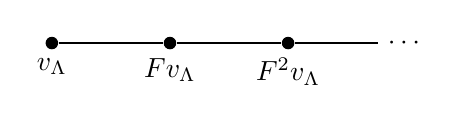
\begin{tikzpicture}[baseline=-3pt,x=1.5cm]
  \foreach \i/\lab in {0/{v_\Lambda},1/{Fv_\Lambda},2/{F^2v_\Lambda}} {
    \node[dot] (n\i) at (\i,0) {};
    \node[below=2pt] at (n\i) {$\lab$};
  }
  \node (n3) at (3,0) {$\cdots$};
  \draw (n0)--(n1)--(n2)--(n3);
\end{tikzpicture}
\]
i.e.\ an infinite string.
\end{example}

\begin{exercise}\leavevmode
\begin{enumerate}
  \item Show that $M(\lambda) = L(\lambda)$ unless $\lambda \in \Z_{\geq 0}$.
  \item If $\lambda \in \Z_{\geq 0}$, show that $M(\lambda)$ contains a unique
    nonzero proper submodule, spanned by $F^{\lambda+1}v_\lambda$,
    $F^{\lambda+2}v_\lambda, \dots$ (which is itself a Verma module). Recover
    the finite-dimensional irreducible representations.
\end{enumerate}
\end{exercise}

\begin{figure}[!htbp]
\centering
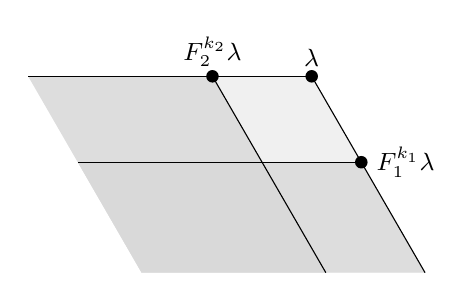
\begin{tikzpicture}[scale=0.9,every node/.append style={font=\small}]
  \coordinate (L) at (0,0);
  \coordinate (A) at (-1.4,0);
  \coordinate (B) at (-60:1.4);
  \fill[gray!12] (L) -- ++(-4,0) -- ++(-60:3.2) -- ($(L)+(-60:3.2)$) -- cycle;
  \fill[gray!30,opacity=0.8] (A) -- ++(-2.6,0) -- ++(-60:3.2) -- ($(A)+(-60:3.2)$) -- cycle;
  \fill[gray!30,opacity=0.8] (B) -- ++(-4,0) -- ++(-60:1.8) -- ($(B)+(-60:1.8)$) -- cycle;
  \draw (L) -- ++(-4,0); \draw (L) -- ++(-60:3.2);
  \draw (A) -- ++(-60:3.2); \draw (B) -- ++(-4,0);
  \foreach \p in {L,A,B} \node[dot] at (\p) {};
  \node[above] at (L) {$\lambda$};
  \node[above] at (A) {$F_2^{k_2}\lambda$};
  \node[right=2pt] at (B) {$F_1^{k_1}\lambda$};
\end{tikzpicture}
\caption{Some of the singular vectors in a Verma module for $\sl_3$; the label
$F_i^{k_i}\lambda$ marks the weight of $F_i^{k_i}v_\lambda$. Note that the
quotient isn't $W$-invariant, so there must be others.}
\label{fig:verma-sl3}
\end{figure}

\begin{exercise}\leavevmode
\begin{enumerate}
  \item If $\g$ is an arbitrary simple Lie algebra and
    $\Lambda(H_i) \in \Z_{\geq 0}$, show that
    $F_i^{\Lambda(H_i)+1} \cdot v_\Lambda$ is a singular vector of
    $M(\Lambda)$. (There will be others! See figure~\ref{fig:verma-sl3}.)
  \item Compute $\ch M(\Lambda)$ for all Verma modules.
\end{enumerate}
\end{exercise}

\lecture{19} We will now try to show that $L(\Lambda)$ is finite-dimensional
if $\Lambda \in P^+$.

\begin{proposition}
If $\Lambda \in P^+$, $L(\Lambda)$ is integrable, i.e.\ the $E_i$ and $F_i$
act locally nilpotently.
\end{proposition}

\begin{proof}
If $V$ is any highest-weight module, $E_i$ acts locally nilpotently (as
$E_iV_\lambda \subseteq V_{\lambda+\alpha_i}$ and the weights of $V$ lie in
$D(\Lambda)$). We must show that $F_i$ acts locally nilpotently.

By the exercise, $F_i^{\Lambda(H_i)+1} \cdot v_\Lambda$ is a singular vector
(or zero). Since $L(\Lambda)$ is irreducible, it has no singular vectors
outside $\C v_\Lambda$, so $F_i^{\Lambda(H_i)+1}v_\Lambda = 0$.

\begin{exercise}\leavevmode
\begin{enumerate}
  \item $a^kb = \sum_{i=0}^k \binom{k}{i}\bigl((\ad a)^ib\bigr)a^{k-i}$.
  \item Using the above and the Serre relations $(\ad e_\alpha)^4e_\beta = 0$,
    show $F_i^Ne_{-\beta_1}\cdots e_{-\beta_r}v_\Lambda = 0$ for $N \gg 0$ by
    induction on $r$. \qedhere
\end{enumerate}
\end{exercise}
\end{proof}

\begin{remark}
In a general Kac--Moody algebra, the Serre relations are no longer
$(\ad e_\alpha)^4e_\beta = 0$, but the exponents are still bounded above, by
$1 - a_{ij}$ for the relevant $i$, $j$ in the generalised Cartan matrix.
\end{remark}

\begin{corollary}
$\dim L(\Lambda)_\mu = \dim L(\Lambda)_{w\mu}$ for all $w \in W$.
\end{corollary}

\begin{proof}
When we were proving Proposition~8.2, we only needed local nilpotence of $E_i$
and $F_i$ to conclude invariance under $w = s_{\alpha_i} = s_i$. Since $W$ is
generated by the $s_i$, we conclude invariance under all of $W$.
\end{proof}

\begin{theorem}[Cartan's theorem]
If $\g$ is finite-dimensional and $\Lambda \in P^+$, then $L(\Lambda)$ is
finite-dimensional.
\end{theorem}

\begin{remark}
This is clear pictorially: $L(\Lambda)$ is $W$-invariant and sits in the cone
$D(\Lambda)$. However, it's faster to work through it formally.
\end{remark}

\begin{proof}
First, we show that if $\alpha \in R^+$ then $e_{-\alpha}$ acts locally
nilpotently on $L(\Lambda)$, i.e.\ all (not just the simple) local
$\sl_2$'s act integrably. In fact, $e_{-\alpha}^nv_\Lambda = 0$ for
$n = (\Lambda, \alpha\cv) + 1$, since otherwise we have
$L(\Lambda)_{\Lambda - n\alpha} \neq 0$ and hence $s_\alpha(\Lambda - n\alpha)$
is a weight of $L(\Lambda)$. However,
\[
  s_\alpha(\Lambda - n\alpha) = s_\alpha(\Lambda) + n\alpha
    = \Lambda - (\Lambda, \alpha\cv)\alpha + \bigl((\Lambda, \alpha\cv) + 1\bigr)\alpha
    = \Lambda + \alpha > \Lambda,
\]
and so it cannot be a weight in $L(\Lambda)$, as $\Lambda$ is the highest
weight. Applying Exercise~87, we see that $e_{-\alpha}$ acts locally
nilpotently on all of $L(\Lambda)$.

Therefore,
\[
  L(\Lambda) = \U(\fn^-)v_\Lambda
    = \Span\setc{e_{-\beta_1}^{k_1}\cdots e_{-\beta_r}^{k_r}v_\Lambda}{k_i \geq 0},
    \qquad R^+ = \{\beta_1, \dots, \beta_r\},
\]
and only finitely many of these spanning vectors are nonzero, so $L(\Lambda)$
is finite-dimensional.
\end{proof}

\begin{lemma}
$s_i(R^+ \setminus \{\alpha_i\}) = R^+ \setminus \{\alpha_i\}$.
\end{lemma}

\begin{proof}
Let $\alpha \in R^+ \setminus \{\alpha_i\}$,
$\alpha = \sum_{j \neq i} k_j\alpha_j + k_i\alpha_i$ with all $k_j \geq 0$ and
some $k_j \neq 0$ for $j \neq i$ (since the only multiples of $\alpha_i$ in $R$
are $\pm\alpha_i$). Note that $s_i(\alpha)$ has the same coefficients on the
$\alpha_j$ for $j \neq i$. Since $R = R^+ \sqcup -R^+$, we see
$s_i(\alpha) \notin -R^+ \implies s_i(\alpha) \in R^+$; and
$s_i(\alpha) \neq \alpha_i$ since $s_i(\alpha_i) = -\alpha_i \neq \alpha$.
\end{proof}

\begin{lemma}
Recall $\rho = \frac12 \sum_{\alpha \in R^+} \alpha$. Then $\rho(H_i) = 1$ for
all $i$, i.e.\ $\rho = \omega_1 + \dots + \omega_l$.
\end{lemma}

\begin{proof}
Observe
\[
  s_i\rho = s_i\Bigl(\frac12\alpha_i + \frac12\sum_{\substack{\alpha \neq \alpha_i\\ \alpha \in R^+}} \alpha\Bigr)
    = -\frac12\alpha_i + \frac12\sum_{\substack{\alpha \neq \alpha_i\\ \alpha \in R^+}} \alpha
    = \rho - \alpha_i.
\]
On the other hand, $s_i\rho = \rho - (\rho, \alpha_i\cv)\alpha_i$, so
$(\rho, \alpha_i\cv) = 1$ for all $i$.
\end{proof}

\begin{lemma}[Key lemma]
Let $\Lambda \in P^+$, $\mu + \rho \in P^+$, $\mu \leq \Lambda$. If
$|\Lambda + \rho| = |\mu + \rho|$ then $\Lambda = \mu$.
\end{lemma}

\begin{remark}
This, again, is geometrically obvious from the fact that both $D(\Lambda)$ and
a sphere are convex.
\end{remark}

\begin{proof}
\[
  0 = (\Lambda + \rho, \Lambda + \rho) - (\mu + \rho, \mu + \rho)
    = \bigl(\Lambda - \mu, (\Lambda + \rho) + (\mu + \rho)\bigr).
\]
Write $\Lambda - \mu = \sum k_i\alpha_i$ with $k_i \geq 0$. Since
$\Lambda + (\mu + \rho) \in P^+$ and $(\rho, \alpha_i) > 0$ for all $i$, each
$\bigl(\alpha_i, (\Lambda + \rho) + (\mu + \rho)\bigr)$ is positive, so we
must have $k_i = 0$ for all $i$.
\end{proof}

\begin{theorem}[Weyl's complete reducibility theorem]
Let $\g$ be a semisimple Lie algebra over a field $k$ with $\charac k = 0$ and
$k = \overline{k}$. Then every finite-dimensional $\g$-module $V$ is a direct
sum of irreducibles.
\end{theorem}

\begin{proof}
Recall that $\at$ acts diagonalisably on $V$ (since $V$ is completely
reducible as an $(\sl_2)_\alpha$-module for each $\alpha$),
$V = \bigoplus V_\lambda$.

Consider $V^{\fn^+} = \setc{x \in V}{\fn^+x = 0}$. By Engel's theorem,
$V^{\fn^+} \neq 0$. Since $[\at, \fn^+] \subseteq \fn^+$, $\at$ acts on
$V^{\fn^+}$, so $V^{\fn^+} = \bigoplus_{\mu \in P} V_\mu^{\fn^+}$.

\begin{claim}
For every nonzero $v_\mu \in V_\mu^{\fn^+}$, the module $L = \U\g \cdot v_\mu$
is irreducible.
\end{claim}

\begin{proof}
$L$ is a highest weight module with highest weight $\mu$, so we must only show
that it has no other singular vectors. If $\lambda$ is the weight of a singular
vector in $L$, then $\lambda \leq \mu$, but $|\lambda + \rho| = |\mu + \rho|$
by considering the action of the Casimir. Since $V$, and therefore $L$, is
finite-dimensional, we must have $\lambda, \mu \in P^+$, so in particular
$\lambda + \rho \in P^+$. By the key lemma, $\lambda = \mu$.
\end{proof}

Consequently, $V' = \U\g \cdot V^{\fn^+}$ is completely reducible: if
$\{v_1, \dots, v_r\}$ is a weight basis for $V^{\fn^+}$ with weights
$\lambda_1, \dots, \lambda_r$, then $V' = L(\lambda_1) + \dots + L(\lambda_r)$
is a sum of irreducible submodules, and hence a direct sum of some of them.
It remains to show that $N = V/V' = 0$.

Suppose not. $N$ is finite-dimensional, so $N^{\fn^+} \neq 0$. Let
$v_\lambda \in N_\lambda^{\fn^+}$ be a singular vector, so $\lambda \in P^+$.
Lift $v_\lambda$ to $\overline{v_\lambda} \in V_\lambda$. Since
$v_\lambda \neq 0$ in $N$, $\overline{v_\lambda} \notin V^{\fn^+}$, so we must
have $E_i\overline{v_\lambda} \neq 0 \in V_{\lambda+\alpha_i}$ for some $i$.

Note that $E_iv_\lambda = 0$, so $E_i\overline{v_\lambda} \in V'$.
Consequently, the Casimir $\Omega$ acts on $E_i\overline{v_\lambda}$ by
$|\overline{\lambda} + \rho|^2 - |\rho|^2$ for some
$\overline{\lambda} \in \{\lambda_1, \dots, \lambda_r\}$ (looking at a
summand $L(\overline\lambda)$ of $V'$ in which $E_i\overline{v_\lambda}$ has a
nonzero component). On the other hand, since $v_\lambda$ was singular in $N$,
$\Omega$ acts on $v_\lambda$ by $|\lambda + \rho|^2 - |\rho|^2$. Since $\Omega$
commutes with $E_i$, we find $|\overline{\lambda} + \rho| = |\lambda + \rho|$.
Moreover, $\lambda + \alpha_i$ is a weight in $L(\overline{\lambda})$, so
$\lambda + \alpha_i = \overline{\lambda} - \sum k_j\alpha_j$, i.e.\
$\lambda < \overline{\lambda}$. This, however, contradicts the key lemma.
\end{proof}

\begin{remark}
The usual proof (in particular, Weyl's own proof) of this theorem involves
lifting the integrable action to the group, and using the maximal compact
subgroup (for which we have complete reducibility because it has positive,
finite measure). Somehow, the key lemma is the equivalent of a positive-definite
metric.
\end{remark}

\begin{lemma}
Let $\Lambda \in \at^*$ and $M(\Lambda)$ the Verma module. Then
\[
  \ch M(\Lambda) = \frac{e^\Lambda}{\prod_{\alpha \in R^+} (1 - e^{-\alpha})}.
\]
\end{lemma}

\lecture{20}

\begin{proof}
Let $R^+ = \{\beta_1, \dots, \beta_r\}$. By PBW, the basis for $M(\Lambda)$ is
$\setc{e_{-\beta_1}^{k_1}\cdots e_{-\beta_r}^{k_r}v_\Lambda}{k_i \in \Z_{\geq 0}}$,
and the weight of such an element is $\Lambda - \sum k_i\beta_i$. Therefore,
$\dim M(\Lambda)_{\Lambda - \beta}$ is the number of ways of writing $\beta$
as $\sum k_i\beta_i$ over $\beta_i \in R^+$. This is precisely the coefficient
of $e^{-\beta}$ in $\prod_{\alpha \in R^+} (1 - e^{-\alpha})^{-1}$.
\end{proof}

Write $\Delta = \prod_{\alpha \in R^+} (1 - e^{-\alpha})$. We have shown that
$\ch M(\Lambda) = e^\Lambda/\Delta$.

\begin{lemma}
For all $w \in W$, $w(e^\rho\Delta) = \det w \cdot e^\rho\Delta$. Here,
$\det\colon W \to \{\pm 1\}$ gives the determinant of $w$ acting on $\at^*$.
\end{lemma}

\begin{proof}
Since $W$ is generated by simple reflections, it suffices to check that
$s_i(e^\rho\Delta) = -e^\rho\Delta$. Indeed,
\[
  s_i(e^\rho\Delta)
  = s_i\Bigl(e^\rho(1 - e^{-\alpha_i})\prod_{\substack{\alpha \neq \alpha_i\\ \alpha \in R^+}} (1 - e^{-\alpha})\Bigr)
  = e^{\rho - \alpha_i}(1 - e^{\alpha_i})\prod_{\substack{\alpha \neq \alpha_i\\ \alpha \in R^+}} (1 - e^{-\alpha})
  = -e^\rho\Delta. \qedhere
\]
\end{proof}

\begin{lemma}\leavevmode
\begin{enumerate}
  \item For any highest weight module $V(\Lambda)$ with highest weight
    $\Lambda$ there exist coefficients $a_\lambda \geq 0$, $\lambda \leq \Lambda$,
    such that
    \[
      \ch V(\Lambda) = \sum_{\substack{\lambda \leq \Lambda\\ |\lambda + \rho| = |\Lambda + \rho|}} a_\lambda \ch L(\lambda),
    \]
    with $a_\Lambda = 1$.
  \item There exist coefficients $b_\lambda \in \Z$ with $b_\Lambda = 1$ such
    that
    \[
      \ch L(\Lambda) = \sum_{\substack{\lambda \leq \Lambda\\ |\lambda + \rho| = |\Lambda + \rho|}} b_\lambda \ch M(\lambda).
    \]
\end{enumerate}
\end{lemma}

We write
$B(\Lambda) = \setc{\lambda \leq \Lambda}{|\lambda + \rho| = |\Lambda + \rho|}$.
Recall that $B(\Lambda)$ is a finite set.

\begin{remark}
We have shown that $B(\Lambda)$ is finite when $\Lambda \in \R R$, but it is
true in general.
\end{remark}

\begin{proof}
First, note that (1) implies (2). Indeed, totally order $B(\Lambda)$ so that
$\lambda_i \leq \lambda_j \implies i \leq j$. Applying (1) to the Verma
modules gives a system of equations relating the $\ch M(\lambda)$ and the
$\ch L(\lambda)$ which is upper-triangular with $1$'s on the diagonal.
Inverting this system gives (2). (Note in particular that the coefficients in
(2) may be negative.)

We now prove (1). Recall that the weight spaces of a highest weight module are
finite-dimensional. We induct on $\sum_{\mu \in B(\Lambda)} \dim V(\Lambda)_\mu$.

If $V(\Lambda)$ is irreducible, we clearly have (1). Otherwise, there exists
$\mu \in B(\Lambda)$, $\mu \neq \Lambda$, with a singular vector
$v_\mu \in V(\Lambda)_\mu$. Pick such a $\mu$ with the largest height of
$\Lambda - \mu$ (recall the height of $\sum k_i\alpha_i$ is $\sum k_i$). Then
$\U\g \cdot v_\mu \subseteq V(\Lambda)$ has no singular vectors other than
those in its highest weight space, and is therefore irreducible, $L(\mu)$.
Setting $\overline{V(\Lambda)} = V(\Lambda)/L(\mu)$, we see that
$\overline{V(\Lambda)}$ is a highest-weight module with a smaller value of
$\sum_{\mu \in B(\Lambda)} \dim \overline{V(\Lambda)}_\mu$, and
$\ch V(\Lambda) = \ch \overline{V(\Lambda)} + \ch L(\mu)$.
\end{proof}

We will now compute $\ch L(\Lambda)$ for $\Lambda \in P^+$. We know
\[
  \ch L(\Lambda) = \sum_{\lambda \in B(\Lambda)} b_\lambda \ch M(\lambda)
    = \sum_{\lambda \in B(\Lambda)} b_\lambda e^\lambda/\Delta.
\]
Now, $w(\ch L(\Lambda)) = \ch L(\Lambda)$ for all $w \in W$, and
$w(\Delta e^\rho) = \det w \cdot \Delta e^\rho$. Therefore,
\[
  e^\rho\Delta \ch L(\Lambda) = \sum_{\lambda \in B(\Lambda)} b_\lambda e^{\lambda+\rho}
\]
is $W$-antiinvariant. We can therefore rewrite
\[
  \sum_{\lambda \in B(\Lambda)} b_\lambda e^{\lambda+\rho}
  = \sum_{\text{orbits of } W \text{ on } B(\Lambda) + \rho} b_\lambda
    \sum_{w \in W} \det w \cdot e^{w(\lambda+\rho)}.
\]
Now, if $\lambda \in \R R$ (which is true, since $\Lambda \in P^+$), then
$W(\lambda + \rho)$ intersects
$\setc{x \in \R R}{(x, \alpha_i\cv) \geq 0 \ \forall i}$ in exactly one point
(this set is a fundamental domain for the $W$-action, and we won't have
boundary problems because $(\rho, \alpha_i\cv) = 1 > 0$). Therefore, we can
take a dominant weight as the orbit representative. Note, however, that there
is only one $\lambda \in B(\Lambda)$ with $\lambda + \rho$ dominant, namely
$\Lambda$! (This was the Key Lemma~10.10.) Therefore, we derive

\begin{theorem}[Weyl character formula]
\[
  \boxed{\ch L(\Lambda)
    = \frac{\sum_{w \in W} \det w \cdot e^{w(\Lambda+\rho)}}{e^\rho\prod_{\alpha \in R^+} (1 - e^{-\alpha})}
    = \sum_{w \in W} \det w \cdot \ch M\bigl(w(\Lambda + \rho) - \rho\bigr).}
\]
\end{theorem}

\begin{example}
Let $\g = \sl_2$, and write $z = e^{\alpha/2}$. Then $\C[P] = \C[z, z^{-1}]$
and $e^\rho = z$. We have
\[
  \ch L(m\alpha/2) = (z^{m+1} - z^{-(m+1)})/(z - z^{-1})
\]
as before.
\end{example}

\begin{remark}
The second expression for the character of $L(\Lambda)$ looks like an Euler
characteristic. In fact, it is: there is a complex of Verma modules whose
cohomology is the irreducible module. This is known as the
``Bernstein--Gelfand--Gelfand'' resolution.

The first expression comes from something like a cohomology of coherent line
bundles, and is variously known as Euler--Grothendieck, Atiyah--Bott, and
Atiyah--Singer.
\end{remark}

\begin{corollary}
Since $L(0) = \C$, we must have $\ch L(0) = 1$, so
\[
  e^\rho\prod_{\alpha \in R^+} (1 - e^{-\alpha}) = \sum_{w \in W} \det w \cdot e^{w\rho}.
\]
This is known as the \emph{Weyl denominator identity}.
\end{corollary}

\begin{exercise}
Let $\g = \sl_n$. Show that the Weyl denominator identity is equivalent to the
Vandermonde determinant
\[
  \det \begin{pmatrix}
    1 & 1 & \cdots & 1\\
    z_1 & z_2 & \cdots & z_n\\
    \vdots & \vdots & \ddots & \vdots\\
    z_1^{n-1} & z_2^{n-1} & \cdots & z_n^{n-1}
  \end{pmatrix} = \prod_{i<j} (z_j - z_i),
\]
where we write $z_i = e^{e_i}$.
\end{exercise}

\begin{corollary}[Weyl dimension formula]
\[
  \dim L(\Lambda) = \prod_{\alpha \in R^+} \frac{(\alpha, \Lambda + \rho)}{(\alpha, \rho)}.
\]
\end{corollary}

\begin{example}
$\g = \sl_3$ of type $A_2$, $R^+ = \{\alpha, \beta, \alpha + \beta\}$ with
$\rho = \alpha + \beta = \omega_1 + \omega_2$. Let
$\Lambda = m_1\omega_1 + m_2\omega_2$; then
\[
  \begin{array}{c|c|c|c}
    & \alpha & \beta & \alpha + \beta\\ \hline
    (\,\cdot\,, \Lambda + \rho) & m_1 + 1 & m_2 + 1 & m_1 + m_2 + 2\\
    (\,\cdot\,, \rho) & 1 & 1 & 2
  \end{array}
\]
Therefore, the dimension of $L(\Lambda)$ is
$\frac12(m_1 + 1)(m_2 + 1)(m_1 + m_2 + 2)$.
\end{example}

``Just to check that you too certainly know the dimensions of the irreducible
representations, let me state the obvious exercise.''

\begin{exercise}
Compute the dimensions of all the finite-dimensional irreducible
representations of $B_2$ and $G_2$.
\end{exercise}

\lecture{21}

\begin{remark}
Let $w \in W$ be written as $w = s_{i_1}s_{i_2}\cdots s_{i_r}$ where the
$s_{i_k}$ are simple reflections. Then $\det w = (-1)^r$. The minimal $r$ such
that $w$ can be written in this form is called the \emph{length} of $w$,
denoted $l(w)$. The \emph{Monoid Lemma} (also known as Matsumoto's theorem)
asserts that you can get from one minimal-length expression for $w$ to
another by repeatedly applying the braid relations.
\end{remark}

\begin{exercise}
$l(w) = \#\{-R^+ \cap w^{-1}R^+\} = l(w^{-1})$.
\end{exercise}

We now go back to our proof of the Weyl dimension formula.

\begin{proof}
We know $\ch L(\Lambda) = \sum \dim L(\Lambda)_\lambda e^\lambda \in \C[P]$. We
would like to set $e^\lambda \mapsto 1$, but that leads to a $0/0$ expression
in the Weyl character formula, which is hard to evaluate. Therefore, we will
start by defining the homomorphism $F_\mu\colon \C[P] \to \C(q)$,
$e^\lambda \mapsto q^{-(\lambda, \mu)}$. We would like to evaluate
$F_0(\ch L(\Lambda))$, since $F_0(e^\mu) = 1$ for all $\mu$.

We apply $F_\mu$ to the Weyl denominator identity:
\[
  q^{-(\rho, \mu)}\prod_{\alpha \in R^+} (1 - q^{(\alpha, \mu)})
  = \sum_{w \in W} \det w \, q^{-(w\rho, \mu)}
  = \sum_{w \in W} \det w \, q^{-(\rho, w^{-1}\mu)},
\]
since $\det w = \det w^{-1}$ and $(x, wy) = (w^{-1}x, y)$ (i.e.\ the Weyl group
is a subgroup of the orthogonal group of the inner product).

We now apply $F_\mu$ to the Weyl character formula:
\[
  F_\mu(\ch L(\Lambda))
  = \frac{\sum_{w \in W} \det w \, q^{-(w(\Lambda+\rho), \mu)}}{q^{-(\rho, \mu)}\prod_{\alpha \in R^+} (1 - q^{(\alpha, \mu)})},
\]
provided $(\alpha, \mu) \neq 0$ for all $\alpha \in R^+$.

Take $\mu = \rho$ (recall that $(\rho, \alpha_i) > 0$ for all simple roots
$\alpha_i$, so $(\rho, \alpha) > 0$ for all $\alpha \in R^+$). Then
\[
  F_\rho(\ch L(\Lambda)) = \sum \dim L(\Lambda)_\lambda q^{-(\lambda, \rho)}
  = \frac{q^{-(\rho, \Lambda+\rho)}\prod_{\alpha \in R^+} (1 - q^{(\alpha, \Lambda+\rho)})}
         {q^{-(\rho, \rho)}\prod_{\alpha \in R^+} (1 - q^{(\alpha, \rho)})},
\]
where we used our expression for the Weyl denominator identity, with
$\mu = \Lambda + \rho$, to rewrite the numerator.

Setting $q = 1$ and applying L'H\^opital's rule,
\[
  \dim L(\Lambda) = \prod_{\alpha \in R^+} \frac{(\Lambda + \rho, \alpha)}{(\rho, \alpha)}. \qedhere
\]
\end{proof}

\begin{remark}
``You are now in a position to answer any question you choose to answer, if
necessary by brute force.'' For example, let us decompose
$L(\lambda) \otimes L(\mu) = \sum m_{\lambda\mu}^\nu L(\nu)$; we want to
compute the \emph{Littlewood--Richardson coefficients} $m_{\lambda\mu}^\nu$
(recall that we had the Clebsch--Gordan rule for them in $\sl_2$).

Define $\overline{\phantom{x}}\colon \Z[P] \to \Z[P]$, $e^\lambda \mapsto e^{-\lambda}$,
and $\CT\colon \Z[P] \to \Z$ with $e^\lambda \mapsto 0$ unless $\lambda = 0$,
and $e^0 \mapsto 1$. Define $(\,,\,)\colon \Z[P] \times \Z[P] \to \Z$ by
$(f, g) = \frac{1}{|W|}\CT(f\overline{g}\Delta\overline{\Delta})$, where
$\Delta = \prod_{\alpha \in R^+} (1 - e^{-\alpha})$.
\end{remark}

\begin{claim}
Let $\chi_\lambda = \ch L(\lambda)$, $\chi_\mu = \ch L(\mu)$; then
$(\chi_\lambda, \chi_\mu) = \delta_{\lambda\mu}$. (If our Lie algebra has type
$A$, then the $\chi_\lambda$ are the Schur functions, and this is their
orthogonality.)
\end{claim}

Given this claim, $m_{\lambda\mu}^\nu = (\chi_\lambda\chi_\mu, \chi_\nu)$ is
algorithmically computable. It was a great surprise to everyone when it was
discovered that there is a simpler and more beautiful way of doing this.

\begin{proof}[Proof of claim]
By the Weyl character formula, $\chi_\lambda\Delta = \sum_{w \in W} \det w\,
e^{w(\lambda+\rho) - \rho}$. Therefore
\[
  (\chi_\lambda, \chi_\mu) = \frac{1}{|W|}\CT\Bigl(\sum_{x, w \in W}
    e^{w(\lambda+\rho) - \rho}\,\overline{e^{x(\mu+\rho) - \rho}}\det(wx)\Bigr).
\]
However, $\CT(e^{w(\lambda+\rho) - x(\mu+\rho)}) = \delta_{wx}\delta_{\mu\lambda}$,
since for $\lambda, \mu \in P^+$ we have
$x^{-1}w(\lambda + \rho) = \mu + \rho \implies x = w,\ \lambda = \mu$.
\end{proof}

\section{Principal \texorpdfstring{$\sl_2$}{sl(2)}}

Define $\rho^L \in \at^*$ by $(\rho^L, \alpha_i) = 1$ for all
$\alpha_i \in \Pi$. (Compare with $\rho$, which had $(\rho, \alpha_i\cv) = 1$.)

\begin{exercise}
Show $\rho^L = \frac12\sum_{\alpha \in R^+} \alpha\cv$. In particular, if $R$
is simply laced and normalised so that $(\alpha, \alpha) = 2$, then
$\rho = \rho^L$.
\end{exercise}

Then $(\rho^L, \alpha) = \htt(\alpha) = \sum k_i$ if we write
$\alpha = \sum k_i\alpha_i$.

\begin{exercise}
\[
  F_{\rho^L}(\ch L(\Lambda)) = q^{-(\Lambda, \rho^L)}\prod_{\alpha \in R^+}
    \frac{1 - q^{(\Lambda+\rho, \alpha\cv)}}{1 - q^{(\rho, \alpha\cv)}}.
\]
[\emph{Hint:} apply $F_{\rho^L}$ to the Weyl denominator identity for the
\emph{Langlands dual Lie algebra}, with root system $R\cv$.]
\end{exercise}

Note that $(\lambda + \rho, \alpha\cv)/(\rho, \alpha\cv) = (\lambda + \rho, \alpha)/(\rho, \alpha)$
as $\alpha\cv = 2\alpha/(\alpha, \alpha)$, so we recovered the same formula
for the Weyl dimension.

\begin{definition}
We call $F_{\rho^L}(\ch L(\Lambda))$ the \emph{$q$-dimension} of $L(\Lambda)$,
denoted $\dimq L(\Lambda)$.
\end{definition}

\begin{proposition}
$\dimq L(\Lambda)$ is a unimodal polynomial. More specifically, it lives in
$\N[q, q^{-1}]^{\Z/2}$ or $q^{1/2}\N[q, q^{-1}]^{\Z/2}$ (depending on its
degree), where $\Z/2$ acts by $q \mapsto q^{-1}$, and the coefficients
decrease as the absolute value of the degree gets bigger.
\end{proposition}

\begin{proof}
We will show that $\dimq L(\Lambda)$ is the character of an $\sl_2$-module in
which all ``strings'' have the same parity.

Set $H = 2\nu^{-1}(\rho^L) \in \at \subseteq \g$, and set $E = \sum E_i$.

\begin{exercise}
Check that $[H, E] = 2E$.
\end{exercise}

Writing $H = \sum c_iH_i$ with $c_i \in \C$, set $F = \sum c_iF_i$.

\begin{exercise}\leavevmode
\begin{enumerate}
  \item Show that $E, F, H$ span a copy of $\sl_2$. This is called the
    \emph{principal $\sl_2$}.
  \item Show that if $\Lambda - \gamma$ is a weight of $L(\Lambda)$, then
    $(\Lambda - \gamma, 2\rho^L) \equiv (\Lambda, 2\rho^L) \bmod 2$.
  \item Derive the proposition. (The eigenvalue of $H$ on $L(\Lambda)_\lambda$
    is $(\lambda, 2\rho^L)$, twice the exponent of $q^{-1}$ in
    $F_{\rho^L}(e^\lambda)$.) \qedhere
\end{enumerate}
\end{exercise}
\end{proof}

\begin{exercise}
Write $[n] = (q^n - 1)/(q - 1)$, and $[n]! = [n][n-1]\cdots[1]$. Show that the
following polynomials are unimodal:
\[
  \begin{bmatrix} n \\ k \end{bmatrix} = \frac{[n]!}{[k]!\,[n-k]!}, \qquad
  (1 + q)(1 + q^2)\cdots(1 + q^n).
\]
[\emph{Hint:} for the first, apply the above arguments to $\g = \sl_n$ and
$V = \Lambda^k\C^n$, or to $\g = \sl_{n-k+1}$ and $V = S^k\C^{n-k+1}$. For
the second, apply it to the spin representation of $B_n = \so_{2n+1}$; we will
define the spin representation next time.]
\end{exercise}

\begin{remark}
When is $L(\lambda) \cong L(\lambda)^*$? Precisely when the lowest weight of
$L(\lambda)$ is $-\lambda$. The lowest weight of $L(\lambda)$ is $w_0\lambda$,
where $w_0$ is the (unique) maximal-length element of $W$, which sends all the
positive roots to negative ones.

Now, for a representation $V$ which is isomorphic to its dual $V^*$, we get a
nondegenerate invariant bilinear form on $V$. If $V$ is irreducible, this
bilinear form is either symmetric or antisymmetric. By the above, we see that
we can determine which it is by laboriously computing characters; but can we
tell simply by looking at $\lambda$?

The answer turns out to be yes. Indeed, the form will pair the highest-weight
and the lowest-weight vector, and if we look at the principal $\sl_2$, it is a
string from the highest-weight to the lowest-weight vector. Now, on the
principal $\sl_2$ it is quite easy to see that the form is antisymmetric if the
representation is $L(n)$ with $n$ odd, and symmetric if it is $L(n)$ with $n$
even. Thus, all we need to know is (the parity of) $(\lambda, 2\rho^L)$. This
is called the \emph{Schur indicator}.
\end{remark}

\lecture{22}

\begin{exercise}
Compute $\dimq L(\theta)$, where $L(\theta)$ is the adjoint representation, for
$G_2$, $A_2$, and $B_2$. Then do it for all the classical groups. You will
notice that $L(\theta)|_{\text{principal } \sl_2} = L(2e_1) + \dots + L(2e_l)$,
where $l = \rank \g = \dim \at$, $e_1, \dots, e_l \in \N$, and $e_1 = 1$. The
$e_i$ are called the \emph{exponents of the Weyl group}, and the order of the
Weyl group is $|W| = (e_1 + 1)\cdots(e_l + 1)$. Compute $|W|$ for $E_8$.
\end{exercise}

\section{Crystals}

Let $\g$ be a semisimple Lie algebra, $\Pi = \{\alpha_1, \dots, \alpha_l\}$ the
simple roots, and $P$ the weight lattice.

\begin{definition}
A \emph{crystal} is a set $B$, $0 \notin B$, together with functions
$\wt\colon B \to P$, $\te_i\colon B \to B \sqcup \{0\}$,
$\tf_i\colon B \to B \sqcup \{0\}$ such that
\begin{enumerate}
  \item if $\te_ib \neq 0$, then $\wt(\te_i(b)) = \wt(b) + \alpha_i$; if
    $\tf_ib \neq 0$, then $\wt(\tf_i(b)) = \wt(b) - \alpha_i$;
  \item for $b, b' \in B$, $\te_ib = b'$ if and only if $b = \tf_ib'$;
  \item before we state the third defining property, we need to introduce
    slightly more notation.
\end{enumerate}
\end{definition}

We can draw $B$ as a graph. The vertices are $b \in B$, and the edges are
$b \xrightarrow[i]{} b'$ if $\tf_ib = b'$ (equivalently, $\te_ib' = b$). We say
that this edge is ``coloured by $i$''. This graph is known as the
\emph{crystal graph}.

\begin{example}
In $\sl_2$ the string
\[
  n \to n - 2 \to n - 4 \to \dots \to -n
\]
is a crystal, where the weight of vertex $i$ is $i\alpha/2$.
\end{example}

Define $\epsilon_i(b) = \max\setc{n \geq 0}{\te_i^n(b) \neq 0}$, and
$\phi_i(b) = \max\setc{n \geq 0}{\tf_i^n(b) \neq 0}$:
\[
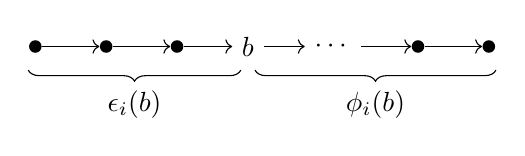
\begin{tikzpicture}[baseline=-3pt,x=0.9cm]
  \foreach \i in {0,1,2} \node[dot] (p\i) at (\i,0) {};
  \node (b) at (3,0) {$b$};
  \node (d) at (4.2,0) {$\cdots$};
  \node[dot] (q) at (5.4,0) {};
  \node[dot] (r) at (6.4,0) {};
  \draw[->] (p0)--(p1); \draw[->] (p1)--(p2); \draw[->] (p2)--(b);
  \draw[->] (b)--(d); \draw[->] (d)--(q); \draw[->] (q)--(r);
  \draw[decorate,decoration={brace,mirror,amplitude=4pt}] (-0.1,-0.3) -- (2.9,-0.3)
    node[midway,below=4pt] {$\epsilon_i(b)$};
  \draw[decorate,decoration={brace,mirror,amplitude=4pt}] (3.1,-0.3) -- (6.5,-0.3)
    node[midway,below=4pt] {$\phi_i(b)$};
\end{tikzpicture}
\]
In $\sl_2$, the sum $\epsilon_i(b) + \phi_i(b)$ is the length of the string
(the number of arrows in it). On the other hand, if we are in the
highest-weight representation $L(n) = L(n\omega)$ and $\wt(b) = n - 2k$, then
$\epsilon(b) = k$ and $\phi(b) = n - k$, i.e.\
$\phi(b) - \epsilon(b) = (\wt(b), \alpha\cv)$. The third defining property of
crystals is that this happens in general:
\begin{enumerate}[start=3]
  \item $\phi_i(b) - \epsilon_i(b) = (\wt(b), \alpha_i\cv)$ for all
    $\alpha_i \in \Pi$.
\end{enumerate}
Define $B_\mu = \setc{b \in B}{\wt(b) = \mu}$.

\begin{definition}
For crystals $B_1$ and $B_2$, we define the tensor product $B_1 \otimes B_2$ as
follows: as a set, $B_1 \otimes B_2 = B_1 \times B_2$,
$\wt(b_1 \otimes b_2) = \wt(b_1) + \wt(b_2)$, and
\begin{align*}
  \te_i(b_1 \otimes b_2) &= \begin{cases}
    (\te_ib_1) \otimes b_2, & \text{if } \phi_i(b_1) \geq \epsilon_i(b_2),\\
    b_1 \otimes (\te_ib_2), & \text{if } \phi_i(b_1) < \epsilon_i(b_2),
  \end{cases}\\
  \tf_i(b_1 \otimes b_2) &= \begin{cases}
    (\tf_ib_1) \otimes b_2, & \text{if } \phi_i(b_1) > \epsilon_i(b_2),\\
    b_1 \otimes (\tf_ib_2), & \text{if } \phi_i(b_1) \leq \epsilon_i(b_2),
  \end{cases}
\end{align*}
where $b \otimes 0 = 0 \otimes b = 0$.
\end{definition}

That is, we are trying to recreate the picture in figure~\ref{fig:crystal-sl2-again}
in each colour.

\begin{exercise}
Check that $B_1 \otimes B_2$ as defined above is a crystal.
\end{exercise}

\begin{exercise}
$B_1 \otimes (B_2 \otimes B_3) \cong (B_1 \otimes B_2) \otimes B_3$ via
$b_1 \otimes (b_2 \otimes b_3) \mapsto (b_1 \otimes b_2) \otimes b_3$.
\end{exercise}

\begin{figure}[!htbp]
  \centering
  \slcrystal
  \caption{Crystal for $\sl_2$ (as in figure~\ref{fig:crystal-sl2}).}
  \label{fig:crystal-sl2-again}
\end{figure}

\begin{remark}
As we see above, the tensor product is associative. In general, however, it is
not commutative.
\end{remark}

\begin{definition}
$B\cv$ is the crystal obtained from $B$ by reversing the arrows. That is,
$B\cv = \setc{b\cv}{b \in B}$, $\wt(b\cv) = -\wt(b)$,
$\epsilon_i(b\cv) = \phi_i(b)$ (and vice versa), and
$\te_i(b\cv) = (\tf_ib)\cv$ (and vice versa).
\end{definition}

\begin{exercise}
$(B_1 \otimes B_2)\cv = B_2\cv \otimes B_1\cv$.
\end{exercise}

\begin{remark}
We will see in a moment precisely how we can attach a crystal to the basis of a
representation. If $B$ parametrises a basis for $V$, then $B\cv$ parametrises a
basis for $V^*$. The condition on the weights can be seen by noting that if
$L(\lambda)$ has highest weight $\lambda$, then $L(\lambda)^*$ has lowest
weight $-\lambda$.
\end{remark}

\begin{theorem}[Kashiwara]
Let $L(\lambda)$ be an irreducible highest-weight representation with highest
weight $\lambda \in P^+$. Then
\begin{enumerate}
  \item There exists a crystal $B(\lambda)$ whose elements are in one-to-one
    correspondence with a basis of $L(\lambda)$, and the elements of
    $B(\lambda)_\mu$ parametrise a basis of $L(\lambda)_\mu$, so that
    \[
      \ch L(\lambda) = \sum_{b \in B(\lambda)} e^{\wt(b)}.
    \]
  \item For any simple root $\alpha_i$ (i.e.\ a simple $\sl_2 \subseteq \g$),
    the decomposition of $L(\lambda)$ as an $(\sl_2)_i$-module is given by the
    $i$-coloured strings in $B(\lambda)$. (In particular, as an uncoloured
    graph, $B(\lambda)$ is connected, since $L(\lambda)$ is spanned by the
    vectors $(\prod f_i)v_\lambda$.)
  \item $B(\lambda) \otimes B(\mu)$ is the crystal for
    $L(\lambda) \otimes L(\mu)$, i.e.\ $B(\lambda) \otimes B(\mu)$ decomposes
    into connected components in the same way as $L(\lambda) \otimes L(\mu)$
    decomposes into irreducible representations.
\end{enumerate}
\end{theorem}

\begin{remark}
We will mention three proof approaches below. The first of them is due to
Kashiwara, and is in the lecturer's opinion the most instructive.
\end{remark}

\begin{example}
Let $\g = \sl_3$, $V = \C^3 = L(\omega_1)$. We compute $V \otimes V$ and
$V \otimes V^*$; see figure~\ref{fig:crystal-sl3}.
\end{example}

\begin{remark}
Note that while the crystals give the decomposition of the representation
into irreducibles, they do not correspond directly to a basis. That is, there
is no basis compatible with all the $(\sl_2)_i$ that we could use here.
Kashiwara's proof of the theorem uses the \emph{quantum group} $\U_q\g$, which
is an algebra over $\C[q, q^{-1}]$ and a deformation of the universal
enveloping algebra $\U\g$. The two have the same representations, but over
$\C[q, q^{-1}]$ there is a very nice basis which satisfies
$e_ib = \te_ib + q \cdot (\text{some mess})$. Therefore, setting $q = 0$
(``freezing'') will give the crystal.
\end{remark}

\begin{figure}[!htbp]
\centering
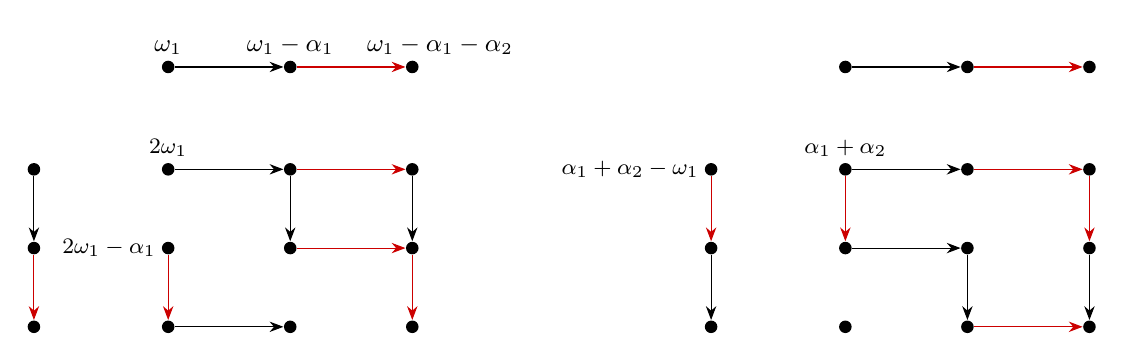
\begin{tikzpicture}[x=1.55cm,y=1cm,every node/.append style={font=\small}]
  % V (x) V. Columns: first factor b_1, b_2, b_3; rows: second factor.
  % Black arrows are f_1, red arrows are f_2.
  \foreach \c in {0,1,2} \node[dot] (t\c) at (\c,1.3) {};
  \draw[cr1] (t0)--(t1); \draw[cr2] (t1)--(t2);
  \node[above=1pt] at (t0) {$\omega_1$};
  \node[above=1pt] at (t1) {$\omega_1 - \alpha_1$};
  \node[above=1pt,xshift=10pt] at (t2) {$\omega_1 - \alpha_1 - \alpha_2$};
  \foreach \r in {0,1,2} \node[dot] (l\r) at (-1.1,-\r) {};
  \draw[cr1] (l0)--(l1); \draw[cr2] (l1)--(l2);
  \foreach \r in {0,1,2} \foreach \c in {0,1,2} \node[dot] (g\r\c) at (\c,-\r) {};
  \draw[cr1] (g00)--(g01); \draw[cr2] (g01)--(g02);
  \draw[cr1] (g01)--(g11); \draw[cr1] (g02)--(g12);
  \draw[cr2] (g11)--(g12); \draw[cr2] (g12)--(g22);
  \draw[cr2] (g10)--(g20); \draw[cr1] (g20)--(g21);
  \node[above=1pt,font=\footnotesize] at (g00) {$2\omega_1$};
  \node[left=1pt,font=\footnotesize] at (g10) {$2\omega_1 - \alpha_1$};
  % V (x) V^*
  \begin{scope}[xshift=8.6cm]
  \foreach \c in {0,1,2} \node[dot] (t\c) at (\c,1.3) {};
  \draw[cr1] (t0)--(t1); \draw[cr2] (t1)--(t2);
  \foreach \r in {0,1,2} \node[dot] (l\r) at (-1.1,-\r) {};
  \draw[cr2] (l0)--(l1); \draw[cr1] (l1)--(l2);
  \node[left=1pt,font=\footnotesize] at (l0) {$\alpha_1 + \alpha_2 - \omega_1$};
  \foreach \r in {0,1,2} \foreach \c in {0,1,2} \node[dot] (g\r\c) at (\c,-\r) {};
  \draw[cr1] (g00)--(g01); \draw[cr2] (g01)--(g02);
  \draw[cr2] (g00)--(g10); \draw[cr2] (g02)--(g12);
  \draw[cr1] (g10)--(g11); \draw[cr1] (g11)--(g21);
  \draw[cr1] (g12)--(g22); \draw[cr2] (g21)--(g22);
  \node[above=1pt,font=\footnotesize] at (g00) {$\alpha_1 + \alpha_2$};
  \end{scope}
\end{tikzpicture}
\caption{Crystals for $V \otimes V$ (left) and $V \otimes V^*$ (right), with
$V = \C^3$. The top row is the crystal of the first factor $V$ and the left
column that of the second factor; black arrows are $\tf_1$ and red arrows are
$\tf_2$. Observe $V \otimes V = S^2V + \Lambda^2V = S^2V + V^*$, and
$V \otimes V^* = \C + \sl_3$.}
\label{fig:crystal-sl3}
\end{figure}

Lusztig's proof uses some of the same ideas, where I didn't catch how it goes.

Soon, we will look at Littelmann paths, which give a purely combinatorial way
of proving this theorem (which, on the face of it, is a purely combinatorial
statement).

\begin{definition}
A crystal is called \emph{integrable} if it is the crystal of a highest-weight
module with highest weight $\lambda \in P^+$.
\end{definition}

For two integrable crystals $B_1$, $B_2$, we do in fact have
$B_1 \otimes B_2 \cong B_2 \otimes B_1$ (in general, this is false).

\begin{remark}
There is a combinatorial condition due to Stembridge which determines whether a
crystal is integrable; it is a degeneration of the Serre relations, but we will
not state it precisely.
\end{remark}

\lecture{23} Consider the crystal for the standard representation of $\sl_n$,
$L(\omega_1) = \C^n$:
\[
  e_1 = \omega_1 \xto{1} \omega_1 - \alpha_1 \xto{2} \omega_1 - \alpha_1 - \alpha_2
  \xto{3} \cdots \xto{n-1} \omega_1 - \alpha_1 - \dots - \alpha_{n-1}.
\]
We can use this to construct the crystals for all representations of $\sl_n$
as follows.

Let $\lambda \in P^+$, $\lambda = k_1\omega_1 + \dots + k_{n-1}\omega_{n-1}$.
Then $L(\lambda)$ must be a summand of
$L(\omega_1)^{\otimes k_1} \otimes \dots \otimes L(\omega_{n-1})^{\otimes k_{n-1}}$,
since the highest weight of this representation is $\lambda$ (with
highest-weight vector $\bigotimes v_{\omega_i}^{\otimes k_i}$, where
$v_{\omega_i}$ is the highest-weight vector of $L(\omega_i)$). Moreover,
$L(\omega_i) = \Lambda^i\C^n$ is a summand of $(\C^n)^{\otimes i}$. We
conclude that $L(\lambda)$ occurs in some $(\C^n)^{\otimes N}$ for $N > 0$.
Therefore, the crystal for $\C^n$ together with the rule for taking tensor
products of crystals determines the crystal of every representation of
$\sl_n$.

We introduce the \emph{semi-standard Young tableaux} of a representation. (This
is due to Hodge, Schur, and Young.) Write
\[
  B(\omega_1) = \bx{1} \xto{1} \bx{2} \xto{2} \bx{3} \xto{3} \cdots \xto{n-1} \bx{n}
\]
for the crystal of the standard representation $\C^n$. For $i < n$ let
\[
  b_i = \bx{1} \otimes \bx{2} \otimes \dots \otimes \bx{i} \in B(\omega_1)^{\otimes i}.
\]
(This corresponds to the vector $v_1 \wedge v_2 \wedge \dots \wedge v_i \in \Lambda^i\C^n$,
where the $v_k$ are the basis vectors of $\C^n$.)

\begin{exercise}\leavevmode
\begin{enumerate}
  \item $b_i$ is a highest-weight vector in $B(\omega_1)^{\otimes i}$ of weight
    $\omega_i = e_1 + \dots + e_i$. (Recall that $b \in B$ is a
    highest-weight vector if $\te_ib = 0$ for all $i$.) Hence, the connected
    component of $B(\omega_1)^{\otimes i}$ containing $b_i$ is $B(\omega_i)$.
  \item This connected component $B(\omega_i)$ consists precisely of
    \[
      \setc{\bx{a_1} \otimes \bx{a_2} \otimes \dots \otimes \bx{a_i}}{1 \leq a_1 < \dots < a_i \leq n}
        \subset B(\omega_1)^{\otimes i}.
    \]
\end{enumerate}
\end{exercise}

We write elements of the form
$\bx{a_1} \otimes \bx{a_2} \otimes \dots \otimes \bx{a_i}$ as column vectors
\[
  \begin{array}{|c|} \hline a_1 \\ \hline a_2 \\ \hline \vdots \\ \hline a_i \\ \hline \end{array}\,.
  \qquad\text{For example, the highest weight vector is denoted}\qquad
  \begin{array}{|c|} \hline 1 \\ \hline 2 \\ \hline \vdots \\ \hline i \\ \hline \end{array}\,.
\]

Let $\lambda = \sum k_i\omega_i$. Embed
$B(\lambda) \hookrightarrow B(\omega_1)^{\otimes k_1} \otimes B(\omega_2)^{\otimes k_2}
\otimes \dots \otimes B(\omega_{n-1})^{\otimes k_{n-1}}$ by mapping the highest
weight vector
$b_\lambda \mapsto b_1^{\otimes k_1} \otimes \dots \otimes b_{n-1}^{\otimes k_{n-1}}$
(which is a highest-weight vector in the image). Now, we can represent any
element in
$B(\omega_1)^{\otimes k_1} \otimes \dots \otimes B(\omega_{n-1})^{\otimes k_{n-1}}$
by a sequence of column vectors as in figure~\ref{fig:tableau}, where the
entries in the boxes are strictly increasing down columns and the columns are
placed side by side with the tensor factors read from right to left.

\begin{figure}[!htbp]
\centering
\begin{tikzpicture}[x=0.5cm,y=0.34cm,every node/.append style={font=\small}]
  % columns of height 7 (k_{n-1} = 3), 6 (k_{n-2} = 2), 5 (k_{n-3} = 1),
  % ..., 2 (k_2 = 4), 1 (k_1 = 3); long columns on the left
  \foreach \c/\h in {0/7,1/7,2/7,3/6,4/6,5/5} \draw (\c,0) rectangle (\c+1,-\h);
  \node at (7.5,-0.5) {$\cdots$};
  \foreach \c/\h in {10/2,11/2,12/2,13/2,14/1,15/1,16/1} \draw (\c,0) rectangle (\c+1,-\h);
  \node[left] at (-0.3,-3.5) {$n - 1$};
  \foreach \a/\b/\lab/\d in {0/3/{k_{n-1}}/3pt,3/5/{k_{n-2}}/3pt,5/6/{k_{n-3}}/13pt,10/14/{k_2}/3pt,14/17/{k_1}/3pt}
    \draw[decorate,decoration={brace,mirror,amplitude=3pt}] (\a+0.05,-7.5) -- (\b-0.05,-7.5)
      node[midway,below=\d] {$\lab$};
\end{tikzpicture}
\caption{Generic element of
$B(\omega_1)^{\otimes k_1} \otimes \dots \otimes B(\omega_{n-1})^{\otimes k_{n-1}}$,
a.k.a.\ a semi-standard Young tableau. Here $k_{n-1} = 3$, $k_{n-2} = 2$,
$k_{n-3} = 1, \dots, k_2 = 4$, $k_1 = 3$.}
\label{fig:tableau}
\end{figure}

\begin{definition}
A \emph{semi-standard Young tableau of shape $\lambda$} is an array of numbers
with dimensions as above, such that the numbers strictly increase down
columns, and weakly increase along rows from left to right.
\end{definition}

\begin{theorem}[Exercise]\leavevmode
\begin{enumerate}
  \item The connected component of $B(\lambda)$ in
    $B(\omega_1)^{\otimes k_1} \otimes \dots \otimes B(\omega_{n-1})^{\otimes k_{n-1}}$
    consists precisely of the semi-standard Young tableaux of shape $\lambda$.
  \item Describe the action of $\te_i$ and $\tf_i$ explicitly in terms of
    tableaux.
\end{enumerate}
\end{theorem}

We will now construct the Young tableaux for all the classical Lie algebras.

\begin{example}\leavevmode
\begin{itemize}
  \item $\so_{2n+1}$, i.e.\ type $B_n$: for the standard representation
    $\C^{2n+1}$ we have the crystal
    \[
      \bx{1} \xto{1} \bx{2} \xto{2} \bx{3} \xto{3} \cdots \xto{n-1} \bx{n}
      \xto{n} \bx{0} \xto{n} \bx{\overline{n}} \xto{n-1} \cdots \xto{2}
      \bx{\overline{2}} \xto{1} \bx{\overline{1}}.
    \]
  \item $\so_{2n}$ (type $D_n$): the crystal of the standard representation
    $\C^{2n}$ is
    \[
    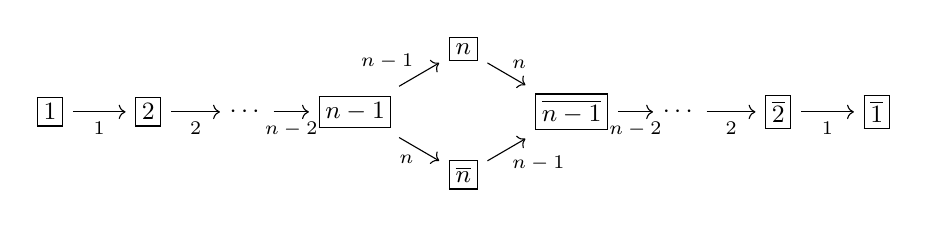
\begin{tikzpicture}[baseline=-3pt,x=1.25cm,every node/.append style={font=\small}]
      \node (1) at (0,0) {\bx{1}};
      \node (2) at (1,0) {\bx{2}};
      \node (d1) at (2,0) {$\cdots$};
      \node (m) at (3.1,0) {\bx{n-1}};
      \node (n) at (4.2,0.8) {\bx{n}};
      \node (nb) at (4.2,-0.8) {\bx{\overline{n}}};
      \node (mb) at (5.3,0) {\bx{\overline{n-1}}};
      \node (d2) at (6.4,0) {$\cdots$};
      \node (2b) at (7.4,0) {\bx{\overline{2}}};
      \node (1b) at (8.4,0) {\bx{\overline{1}}};
      \draw[->] (1) -- node[below]{\scriptsize $1$} (2);
      \draw[->] (2) -- node[below]{\scriptsize $2$} (d1);
      \draw[->] (d1) -- node[below]{\scriptsize $n-2$} (m);
      \draw[->] (m) -- node[above left=-2pt]{\scriptsize $n-1$} (n);
      \draw[->] (m) -- node[below left=-2pt]{\scriptsize $n$} (nb);
      \draw[->] (n) -- node[above right=-2pt]{\scriptsize $n$} (mb);
      \draw[->] (nb) -- node[below right=-2pt]{\scriptsize $n-1$} (mb);
      \draw[->] (mb) -- node[below]{\scriptsize $n-2$} (d2);
      \draw[->] (d2) -- node[below]{\scriptsize $2$} (2b);
      \draw[->] (2b) -- node[below]{\scriptsize $1$} (1b);
    \end{tikzpicture}
    \]
  \item $\spl_{2n}$ (type $C_n$): the crystal of the standard representation
    $\C^{2n}$ is
    \[
      \bx{1} \xto{1} \bx{2} \xto{2} \cdots \xto{n-1} \bx{n} \xto{n}
      \bx{\overline{n}} \xto{n-1} \cdots \xto{2} \bx{\overline{2}} \xto{1}
      \bx{\overline{1}}.
    \]
\end{itemize}
\end{example}

\begin{exercise}\leavevmode
\begin{enumerate}
  \item Check that the crystals of the standard representations are as
    claimed.
  \item What subcategory of the category of representations of $\g$ do these
    representations generate?

    Consider the highest weight $\lambda$ of the standard representation. This
    gives an element $\overline{\lambda} \in P/Q$, a finite group dual to
    $Z(G)$ (where $G$ is the simply connected Lie group attached to $\g$).
    Consider the subgroup $\langle\overline{\lambda}\rangle \leq P/Q$. We
    cannot obtain all of the representations unless $P/Q$ is cyclic and
    generated by $\overline{\lambda}$. For the classical examples we have
    $P/Q = \Z/2 \times \Z/2$ for $D_{2n}$, $\Z/4$ for $D_{2n+1}$, and $\Z/2$
    for $B_n$ and $C_n$.
  \item (Optional) Write down a combinatorial set like Young tableaux that is
    the crystal of $B(\lambda)$ with $\lambda$ obtained from the standard
    representation.
\end{enumerate}
\end{exercise}

For $B_n$ we have one more representation, the \emph{spin representation}.
Recall the Dynkin diagram for $B_n$,
\[
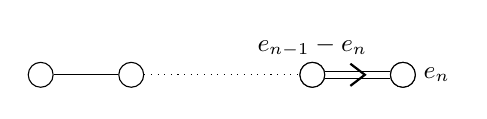
\begin{tikzpicture}[baseline=-3pt,x=1.15cm,every node/.append style={font=\small}]
  \node[node] (b1) at (0,0) {}; \node[node] (b2) at (1,0) {};
  \node[node] (b3) at (3,0) {}; \node[node] (b4) at (4,0) {};
  \draw (b1)--(b2); \draw[dotted] (b2)--(b3); \dbond{b3}{b4}
  \node[node] at (b3) {}; \node[node] at (b4) {};
  \node[above=3pt] at (b3) {$e_{n-1} - e_n$}; \node[right=4pt] at (b4) {$e_n$};
\end{tikzpicture}
\]

\begin{definition}
Let $\omega_1, \dots, \omega_n$ be the dual basis to
$\alpha_1\cv, \dots, \alpha_n\cv$. We call $L(\omega_n)$ the \emph{spin
representation}.
\end{definition}

\begin{exercise}
Use the Weyl dimension formula to show that $\dim L(\omega_n) = 2^n$.
\end{exercise}

Define $B = \setc{(i_1, \dots, i_n)}{i_j = \pm 1}$ with
$\wt((i_1, \dots, i_n)) = \frac12\sum i_je_j \in P$, and
\[
  \te_j(i_1, \dots, i_n) = \begin{cases}
    (i_1, \dots, +1_j, -1_{j+1}, \dots, i_n), & \text{if } (i_j, i_{j+1}) = (-1, +1),\\
    0, & \text{otherwise},
  \end{cases}
  \qquad 1 \leq j \leq n - 1,
\]
and
\[
  \te_n(i_1, \dots, i_n) = \begin{cases}
    (i_1, \dots, i_{n-1}, +1), & \text{if } i_n = -1,\\
    0, & \text{otherwise}
  \end{cases}
\]
(note that in particular $\te_i^2 = 0$ always).

\begin{claim}
This is the crystal of the spin representation $L(\omega_n)$.
\end{claim}

\begin{remark}
Note that $\dim L(\omega_n) = \dim \Lambda^\bullet\C^n$. This is for a very good
reason. Indeed, $\gl_n \subset \so_{2n+1}$ via
\[
  A \mapsto \begin{pmatrix} A & & \\ & 0 & \\ & & -JA^TJ^{-1} \end{pmatrix},
\]
and $L(\omega_n)|_{\gl_n} = \Lambda^\bullet\C^n$ (up to a twist by a
one-dimensional character).
\end{remark}

\begin{exercise}
Check that $B|_{\gl_n}$ is the crystal of $\Lambda^\bullet\C^n$.
\end{exercise}

For type $D_n$, the situation is more complicated. We can define
representations
\[
  V^+ = L(\omega_n), \qquad V^- = L(\omega_{n-1});
\]
these are called the \emph{half-spin} representations. The corresponding
crystals are $B^\pm = \setc{(i_1, \dots, i_n)}{i_j = \pm 1}$ with
$\prod i_j = 1$ for $B^+$ and $\prod i_j = -1$ for $B^-$. We define the weight
and most $\te_i$, $\tf_i$ as before, with the change that
\[
  \te_n(i_1, \dots, i_n) = \begin{cases}
    (i_1, \dots, i_{n-2}, +1, +1), & \text{if } (i_{n-1}, i_n) = (-1, -1),\\
    0, & \text{otherwise}.
  \end{cases}
\]

\lecture{24}

\section{Littelmann paths}

Set $P_\R = P \otimes_\Z \R$. By a \emph{path} we mean a piecewise linear
continuous map $[0, 1] \to P_\R$. We consider paths up to
reparametrisation, i.e.\ $\pi \cong \pi \circ \phi$, where
$\phi\colon [0, 1] \to [0, 1]$ is a piecewise-linear isomorphism. (That is, we
care about the trajectory, not about the speed at which we traverse the path.)

Let $\mathcal{P} = \setc{\text{paths } \pi}{\pi(0) = 0,\ \pi(1) \in P}$. Define
a crystal structure on $\mathcal{P}$ as follows: we set
\[
  \wt(\pi) = \pi(1).
\]
To define $\te_i(\pi)$, let
\[
  h_i = \min\Bigl(\Z \cap \setc{\ip{\pi(t)}{\alpha_i\cv}}{0 \leq t \leq 1}\Bigr) \leq 0.
\]
That is, $h_i$ is the smallest integer in the range of
$t \mapsto \ip{\pi(t)}{\alpha_i\cv}$ (note that since $\pi(0) = 0$, we have
$h_i \leq 0$).

If $h_i = 0$, we set $\te_i(\pi) = 0$ (this is not the path that stays at $0$,
but rather the extra element of the crystal).

If $h_i < 0$, take the smallest $t_1 > 0$ such that
$\ip{\pi(t_1)}{\alpha_i\cv} = h_i$. Then take the largest $t_0 < t_1$ such
that $\ip{\pi(t_0)}{\alpha_i\cv} = h_i + 1$.

The idea is to reflect the segment of the path $\pi$ from $t_0$ to $t_1$ in
the hyperplane $\ip{\lambda}{\alpha_i\cv} = h_i + 1$. Therefore, we define the
path $\te_i(\pi)$ as follows (see figure~\ref{fig:littelmann}):
\[
  \te_i(\pi)(t) = \begin{cases}
    \pi(t), & 0 \leq t \leq t_0,\\
    \pi(t_0) + s_{\alpha_i}(\pi(t) - \pi(t_0))
      = \pi(t) - \ip{\pi(t) - \pi(t_0)}{\alpha_i\cv}\alpha_i, & t_0 \leq t \leq t_1,\\
    \pi(t) + \alpha_i, & t \geq t_1.
  \end{cases}
\]

\begin{figure}[!htbp]
\centering
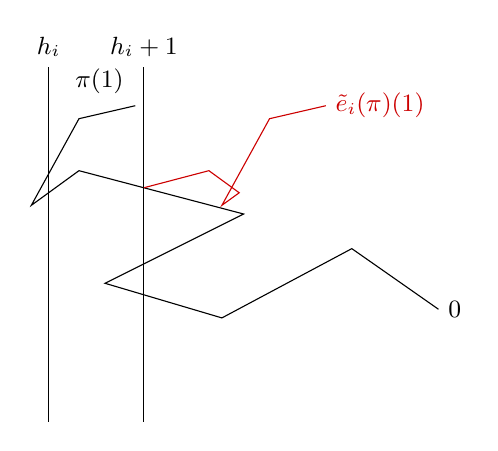
\begin{tikzpicture}[scale=1.1,every node/.append style={font=\small}]
  \draw (0,-2.2) -- (0,1.9) node[above] {$h_i$};
  \draw (1.1,-2.2) -- (1.1,1.9) node[above] {$h_i + 1$};
  % pi, traversed from 0 (bottom right) to pi(1)
  \coordinate (O) at (4.5,-0.9);
  \draw (O) -- (3.5,-0.2) -- (2.0,-1.0) -- (0.65,-0.6) -- (2.25,0.2) -- (0.35,0.7)
        -- (-0.2,0.3) -- (0.35,1.3) -- (1.0,1.45);
  \node[right] at (O) {$0$};
  \node[above left=1pt] at (1.0,1.45) {$\pi(1)$};
  % e_i(pi): reflect the stretch between the last visit to h_i+1 and the
  % first visit to h_i in the line h_i+1, then translate the rest by alpha_i
  % pi meets h_i + 1 for the last time before t_1 at (1.1, 0.503) and first
  % meets h_i at (0, 0.445); alpha_i is drawn as the horizontal vector (2.2, 0)
  \draw[red!80!black] (1.1,0.503) -- (1.85,0.7) -- (2.2,0.445) -- (2.0,0.3)
        -- (2.55,1.3) -- (3.2,1.45);
  \node[red!80!black,right] at (3.2,1.45) {$\te_i(\pi)(1)$};
\end{tikzpicture}
\caption{$\pi$ is drawn in black; $\te_i(\pi)$, from the point where it
deviates from $\pi$, is drawn in red. The vertical lines are the hyperplanes
$\ip{\lambda}{\alpha_i\cv} = h_i$ and $h_i + 1$.}
\label{fig:littelmann}
\end{figure}

\begin{exercise}
Show that $\epsilon_i(\pi) = -h_i$.
\end{exercise}

\begin{example}
Let's compute the crystals of some representations of $\sl_2$. Writing a
straight path by its endpoints,
\[
  \te(0 \to -\alpha/2) = (0 \to \alpha/2), \qquad \te(0 \to \alpha/2) = 0,
\]
and
\[
  \te(0 \to -\alpha) = (0 \to -\alpha/2 \to 0), \qquad
  \te(0 \to -\alpha/2 \to 0) = (0 \to \alpha/2 \to \alpha).
\]
\end{example}

If $\pi$ is a path, let $\pi\cv$ be the reversed path, i.e.\
$t \mapsto \pi(1 - t) - \pi(1)$. Define
\[
  \tf_i(\pi) = \bigl(\te_i(\pi\cv)\bigr)\cv.
\]

\begin{exercise}
With the above definitions, $\mathcal{P}$ is a crystal.
\end{exercise}

Define
$\mathcal{P}^+ = \setc{\text{paths } \pi}{\pi([0, 1]) \subset P_\R^+}$, where
$P_\R^+ = \setc{x \in P_\R}{\ip{x}{\alpha_i\cv} \geq 0 \text{ for all } i}$.
If $\pi \in \mathcal{P}^+$, then $\te_i(\pi) = 0$ for all $i$.

For $\pi \in \mathcal{P}^+$ let $B_\pi$ be the subcrystal of $\mathcal{P}$
generated by $\pi$ (i.e.\ $B_\pi = \{\tf_{i_1}\tf_{i_2}\cdots\tf_{i_r}\pi\} \setminus \{0\}$).

\begin{theorem}[Littelmann]\leavevmode
\begin{enumerate}
  \item If $\pi, \pi' \in \mathcal{P}^+$ then $B_\pi \cong B_{\pi'}$ as
    crystals iff $\pi(1) = \pi'(1)$.
  \item There is a unique isomorphism between this crystal and
    $B(\pi(1))$, the crystal of the irreducible representation
    $L(\pi(1))$. (Of course, the isomorphism sends $\pi$ to the highest-weight
    element of $B(\pi(1))$.)
  \item Moreover, for the path $\pi(t) = \lambda t$, $\lambda \in P^+$,
    Littelmann gives an explicit combinatorial description of the paths in
    $B_\pi$.
\end{enumerate}
\end{theorem}

\begin{example}
Let's compute part of the crystal of the adjoint representation of $\sl_3$,
with simple roots $\alpha$, $\beta$:
\[
  \te_\beta\bigl(0 \to -(\alpha + \beta)\bigr) = (0 \to -\alpha).
\]
\end{example}

\begin{exercise}
Compute the rest of the crystal, and check that you get the adjoint
representation of $\sl_3$.
\end{exercise}

The simplest nontrivial example is $G_2$, the automorphisms of the octonions.

\begin{exercise}
Compute the crystal of the $7$-dimensional and the $14$-dimensional (adjoint)
representations of $G_2$. Compute their tensor product.
\end{exercise}

The tensor product of crystals has a very nice (and natural!) realisation in
terms of concatenating paths:

\begin{definition}
For $\pi_1, \pi_2 \in \mathcal{P}$, define $\pi_1 * \pi_2$ to be the
concatenation (traverse $\pi_1$, then translate $\pi_2$ to start at
$\pi_1(1)$ and traverse it).
\end{definition}

\begin{exercise}
$*\colon \mathcal{P} \otimes \mathcal{P} \to \mathcal{P}$ is a morphism of
crystals.
\end{exercise}

That is, the tensor product of two crystals simply consists of the
concatenated paths in them.

\begin{remark}
We have now defined $B(\lambda)$ explicitly without using $L(\lambda)$. One
can prove the Weyl character formula
\[
  \ch B(\lambda) = \frac{\sum_{w \in W} \det w \, e^{w(\lambda+\rho) - \rho}}{\prod_{\alpha \in R^+} (1 - e^{-\alpha})}
\]
from this, without referring to $L(\lambda)$ or quantum groups. To do this, one
builds $\ch L(\lambda)$ and $L(\lambda)$ itself one root at a time, and uses
the \emph{Demazure character formula}.

More specifically: for each $w \in W$ consider $L_w(\lambda)$, the
$\fn^+$-submodule of $L(\lambda)$ generated by $v_{w\lambda}$, where $v_\lambda$
is the highest weight vector and $v_{w\lambda}$ spans the line
$L(\lambda)_{w\lambda}$. (Equivalently, it is the submodule generated by the
$1$-dimensional space $wL(\lambda)_\lambda$.)
\end{remark}

\begin{theorem}[Demazure character formula]
\[
  \ch L_w(\lambda) = D_w(e^\lambda),
\]
where we write $w = s_{i_1}\cdots s_{i_r}$, a reduced (i.e.\ shortest)
decomposition, and set
\[
  D_w = D_{s_{i_1}}\cdots D_{s_{i_r}}, \qquad
  D_{s_i}(f) = \frac{f - e^{-\alpha_i}s_i(f)}{1 - e^{-\alpha_i}}
    = (1 + s_i)\frac{f}{1 - e^{-\alpha_i}}
    = \frac{f e^{\alpha_i/2} - s_i(f e^{\alpha_i/2})}{e^{\alpha_i/2} - e^{-\alpha_i/2}}.
\]
That is,
\[
  D_{s_i}(e^\lambda) = \begin{cases}
    e^\lambda + e^{\lambda - \alpha_i} + \dots + e^{s_i\lambda}, & \ip{\lambda}{\alpha_i\cv} \geq 0,\\
    0, & \ip{\lambda}{\alpha_i\cv} = -1,\\
    -(e^{\lambda + \alpha_i} + \dots + e^{s_i\lambda - \alpha_i}), & \ip{\lambda}{\alpha_i\cv} < -1.
  \end{cases}
\]
\end{theorem}

``I've got about six minutes. Is that enough time to tell you about the
Langlands program?''

Suppose that $G$ is an algebraic group with Lie algebra $\g$ which is
semisimple. For a given $\g$, there is the smallest group $G$ above it,
$G^{\mathrm{ad}} = G/Z_G$ (whose centre is $\{1\}$). There is also the largest
group, $G^{\mathrm{sc}}$, the simply connected cover of $G$, which is still an
algebraic group. We have $\pi_1(G^{\mathrm{ad}}) \cong (P/Q)^*$ and
$Z_{G^{\mathrm{sc}}} \cong (P/Q)^*$, where $(P/Q)^* = \Hom(P/Q, \C^\times)$
is (non-canonically) isomorphic to $P/Q$.

(For example, $SL_n$ is the simply connected group, and $PSL_n$ is the adjoint
group.)

In this course we have studied the category
$\Rep \g = \Rep G^{\mathrm{sc}}$.

Recall that for $G$ a finite group, the number of irreducible representations
is the number of conjugacy classes, but conjugacy classes do not parametrise
the representations. For us, however, the representations are parametrised
by $P^+ \cong P/W$.

It is possible, for $G$ an algebraic group, to define ${}^LG$, the Langlands
dual group, where the Lie algebra $\g$ and the root system $R$ correspond to
$\g\cv$ and $R\cv$ (and in fact the torus and the dual torus will swap in the
dual group).

If we consider the representations of $G(F)$ where $F = \mathbb{F}_q$ or
$F = \C((t))$, these correspond roughly to conjugacy classes of homomorphisms
$\bigl(W(F) \to {}^LG(\C)\bigr)/{}^LG(\C)$, where $W(F)$ is a ``thickening''
of the Galois group of $F$.


\end{document}
